%%%%%%%%%%%%%%%%%%%%%%%%%%%%%%%%%%%%%%%%%%%%%%%%%%%%%%%%%%%%%%%%%%%%%%%%%%%%%%%
% Titel:   Bericht - Admin
% Autoren: gross10
% Datum:   04.01.2014
% Version: 1.0.0
%%%%%%%%%%%%%%%%%%%%%%%%%%%%%%%%%%%%%%%%%%%%%%%%%%%%%%%%%%%%%%%%%%%%%%%%%%%%%%%
%
%:::Change-Log:::
% Versionierung erfolgt auf folgende Gegebenheiten: -1. Release Versionen
%                                                   -2. Neue Kapitel
%                                                   -3. Fehlerkorrekturen
%
% 0.0.1       Erstellung der Datei
%
%:::Hinweis:::
% Indexerstellung: makeindex -s report.ist report.idx
%   Umlaute m�ssen separat behandelt werden!
%%%%%%%%%%%%%%%%%%%%%%%%%%%%%%%%%%%%%%%%%%%%%%%%%%%%%%%%%%%%%%%%%%%%%%%%%%%%%%%
\documentclass[version=last,fleqn,pointlessnumbers,openright,twoside]{scrreprt}  %first: Ergebniss Kompatibel zu ersten Version; last: Ergebniss entspricht den aktuellen Paketen; fleqn: Formeln linksb�ndig; pointlessnumbers: Kapitelnummerierung ohne Punkt; twoside: Doppelseitiger Druck

%Dokumentangaben
\newcommand{\Titel}{Dokumentation PA1}
\newcommand{\Uebertitel}{Eurobot 2014 Kernteam}
\newcommand{\AutorA}{Hannes Roth}
\newcommand{\AutorB}{Patrick Rohrbach}
\newcommand{\AutorC}{Tobias Meerstetter}
\newcommand{\AutorD}{Simon Grossenbacher}
\newcommand{\DozentA}{Daniel Lanz}
\newcommand{\DozentB}{Ivo Oesch}
\newcommand{\DozentC}{Walter G�ller}
\newcommand{\FachbereichA}{Maschinenbau}
\newcommand{\FachbereichB}{Technik und Informatik}
\newcommand{\Datum}{\the\day.\the\month.\the\year}
\newcommand{\Ort}{Burgdorf}
\newcommand{\Version}{1.0.0}



%%%%%%%%%%%%%%%%%%%%%%%%%%%%%%%%%%%%%%%%%%%%%%%%%%%%%%%%%%%%%%%%%%%%%%%%%%%%%%%
% Pakete
%%%%%%%%%%%%%%%%%%%%%%%%%%%%%%%%%%%%%%%%%%%%%%%%%%%%%%%%%%%%%%%%%%%%%%%%%%%%%%%
%%%%%%%%%%%%%%%%%%%%%%%%%%%%%%%%%%%%%%%%%%%%%%%%%%%%%%%%%%%%%%%%%%%%%%%%%%%%%%%
% Titel:   Bericht - Pakete
% Autor: Simon Grossenbacher  
% Datum:   27.09.2013
% Version: 1.0.0
%%%%%%%%%%%%%%%%%%%%%%%%%%%%%%%%%%%%%%%%%%%%%%%%%%%%%%%%%%%%%%%%%%%%%%%%%%%%%%%
%
%:::Change-Log:::
% Versionierung erfolgt auf folgende Gegebenheiten: -1. Release Versionen
%                                                   -2. Neue Kapitel
%                                                   -3. Fehlerkorrekturen
%
% 0.0.0       Erstellung der Datei
%
%:::Hinweis:::
% Indexerstellung: makeindex -s report.ist report.idx
%   Umlaute m�ssen separat behandelt werden!
%%%%%%%%%%%%%%%%%%%%%%%%%%%%%%%%%%%%%%%%%%%%%%%%%%%%%%%%%%%%%%%%%%%%%%%%%%%%%%%

%Sprach-Optionen
\usepackage[ngerman]{babel} %neue deutsche Rechtschreibung
\usepackage[T1]{fontenc}  %richtige Worttrennung
%\usepackage[applemac]{inputenc}				% Mac - load extended character set (ISO 8859-1)
\usepackage[latin1]{inputenc}  				% Unix/Linux - load extended character set (ISO 8859-1)
%\usepackage[ansinew]{inputenc}  				% Windows - load extended character set (ISO 8859-1)
%\usepackage[utf8]{inputenc}  					% UTF-8 encoding

%Zeilenabstand
\usepackage{setspace}

%Mehr Tabellenoptionen
\usepackage{tabularx}
\usepackage{longtable}
\usepackage{rotating}
\usepackage{multirow}

%Listen
\usepackage{enumitem}

%Besserer Flattersatz
\usepackage{ragged2e}

%Gleiten verhindern
\usepackage{float}
\usepackage{placeins}

%Ueberschriften anpassen
\usepackage{titlesec} 

%Farben
\usepackage{color}
\usepackage{colortbl} %F�r farbige Tabellen

%PDF zu Dokument hinzufuegen
\usepackage[final]{pdfpages}

%Grafiken verwalten
\usepackage{graphicx}
\usepackage[absolute]{textpos}
\usepackage{wrapfig}
\usepackage{subcaption}

%Zeichnen
%\usepackage{pst-pdf}
%\usepackage{pst-all}

%Listnings verwalten
\usepackage{listings}

%Kopf- Fusszeile (Optionen m�ssen direkt �bergeben werden)
\usepackage[automark, %Automatisches aktualisieren der Chapter-Titel
%            headsepline,  %Linie Kopfzeile
%            footsepline,  %Linie fusszeilezeile
%            markuppercase,
            plainfootsepline  %Plain-Style auch mit Linie versehen
            ]{scrpage2}

%Flexible Argumente bei Funktionen
\usepackage{xargs}

%erweiterte Steuerfunktionen
\usepackage{ifthen}

%Index f�r Stichwortverzeichnis
\usepackage{makeidx}

%Index f�r Literaturverzeichnis
\usepackage[babel,german=quotes]{csquotes}
%\usepackage[backend=biber,style=numeric,defernumbers=true,sorting=nyt]{biblatex}
\usepackage[backend=bibtex,defernumbers=true]{biblatex}
\bibliography{bibliography}
\defbibheading{lit}{\section{Literatur}}
\defbibheading{pic}{\section{Abbildungen}}

%Zusaetzliche Symbole direkt im Text
\usepackage{textcomp}
\usepackage{amssymb}

%Einheit kontrolliert eingeben
\usepackage{units}

%dynamische Datumsausgabe
\usepackage[german]{isodate}

%Zusaetzlich Mathemtiksymbole
\usepackage{amsmath}
\usepackage{mathtools}

%Besser Handling von internen Countern und Berechnungen
\usepackage{calc}

%TODOs anbringen am Rand
\usepackage{todonotes}

%Hyperlinks (Muss das letzte geladene Paket sein)
\usepackage[bookmarks=true, %Verzeichnis generieren
            bookmarksopen=true, %Verzeichnis �ffnen
            bookmarksopenlevel=3, %Tiefe der Verzeichnis�ffnung
            unicode=false, %non-Latin Zeichen
            pdftoolbar=true, %PDF-Viewer Toolbar
            pdfmenubar=true, %PDF-Viewer Men�?
            pdffitwindow=true, %Fenster an Seite anpassen beim �ffnen
            pdftitle={\Titel}, %Titel
            %pdfauthor={\Autor1, \Autor2, \Autor3}, %Autor
            pdfsubject={\Uebertitel}, %Thema
%            pdfcreator={\Autor1, \Autor2, \Autor3}, %Ersteller des Dokuments
%            pdfproducer={\Autor1, \Autor2 \Autor3}, %Produzent des Dokuments
            pdfnewwindow=true, %Links in neuem Fenster
            colorlinks=true, %false: Boxen-Links; true: Farben-Links
            linkcolor=red, %Farbe von internen Links
            citecolor=red, %Farbe von Links zu Bibliography
            filecolor=magenta, %Farbe von Links zu Dateien
            urlcolor=blue %Farbe von externen Links
            ]{hyperref}
   
%Querverweise
\usepackage[german]{cleveref}
\usepackage{xr}  %Verweise uber Dokument hinweg

%Besseres Zeichensetzen
\usepackage{microtype}
            
%Glossar/Abk�rzungsverzeichnis
\usepackage[acronym,makeindex]{glossaries}




%%%%%%%%%%%%%%%%%%%%%%%%%%%%%%%%%%%%%%%%%%%%%%%%%%%%%%%%%%%%%%%%%%%%%%%%%%%%%%%
% Funktionen
%%%%%%%%%%%%%%%%%%%%%%%%%%%%%%%%%%%%%%%%%%%%%%%%%%%%%%%%%%%%%%%%%%%%%%%%%%%%%%%
%%%%%%%%%%%%%%%%%%%%%%%%%%%%%%%%%%%%%%%%%%%%%%%%%%%%%%%%%%%%%%%%%%%%%%%%%%%%%%%
% Titel:   Bericht - Funktionen
% Autor:   Simon Grossenbacher  
% Datum:   27.09.2013
% Version: 1.0.0
%%%%%%%%%%%%%%%%%%%%%%%%%%%%%%%%%%%%%%%%%%%%%%%%%%%%%%%%%%%%%%%%%%%%%%%%%%%%%%%
%
%:::Change-Log:::
% Versionierung erfolgt auf folgende Gegebenheiten: -1. Release Versionen
%                                                   -2. Neue Kapitel
%                                                   -3. Fehlerkorrekturen
%
% 0.0.0       Erstellung der Datei
%
%:::Hinweis:::
% Indexerstellung: makeindex -s report.ist report.idx
%   Umlaute m�ssen separat behandelt werden!
%%%%%%%%%%%%%%%%%%%%%%%%%%%%%%%%%%%%%%%%%%%%%%%%%%%%%%%%%%%%%%%%%%%%%%%%%%%%%%%

%%%%%%%%%%%%%%%%%%%%%%%%%%%%%%%%%%%%%%%%%%%%%%%%%%%%%%%%%%%%%%%%%%%%%%%%%%%%%%%
% Text tiefstellen
% param #1 Text
%%%%%%%%%%%%%%%%%%%%%%%%%%%%%%%%%%%%%%%%%%%%%%%%%%%%%%%%%%%%%%%%%%%%%%%%%%%%%%%
\newcommand{\low}[1]{\textsubscript{#1}}



%%%%%%%%%%%%%%%%%%%%%%%%%%%%%%%%%%%%%%%%%%%%%%%%%%%%%%%%%%%%%%%%%%%%%%%%%%%%%%%
% Text hochstellen
% param #1 Text
%%%%%%%%%%%%%%%%%%%%%%%%%%%%%%%%%%%%%%%%%%%%%%%%%%%%%%%%%%%%%%%%%%%%%%%%%%%%%%%
\newcommand{\high}[1]{\textsuperscript{#1}}



%%%%%%%%%%%%%%%%%%%%%%%%%%%%%%%%%%%%%%%%%%%%%%%%%%%%%%%%%%%%%%%%%%%%%%%%%%%%%%%
% Schrift anpassen
% param #1 Schriftfamilie: ptm  Times
%                          phv 	Helvetica
%                          pcr 	Courier
%                          pbk 	Bookman
%                          pag 	Avant Garde
%                          ppl 	Palatino
%                          pch 	Charter
%                          pnc 	New Century Schoolbook
%                          put 	Utopia
% param #2 Strichdicke/Zeichenbreite: b  bold
%                                     m  medium
% param #3 Schriftform: n   normal
%                       it  italic
%                       sl  slanted
%                       sc  small caps
%                       ui  upright italic
% note {\changefont{#1}{#2}{#3} Hallo Welt} Teilbereich aendern
%%%%%%%%%%%%%%%%%%%%%%%%%%%%%%%%%%%%%%%%%%%%%%%%%%%%%%%%%%%%%%%%%%%%%%%%%%%%%%%
\newcommand{\changefont}[3]{\fontfamily{#1} \fontseries{#2} \fontshape{#3} \selectfont}



%%%%%%%%%%%%%%%%%%%%%%%%%%%%%%%%%%%%%%%%%%%%%%%%%%%%%%%%%%%%%%%%%%%%%%%%%%%%%%%
% Zum Beispiel abkuerzen ohne Trennung
% param none
%%%%%%%%%%%%%%%%%%%%%%%%%%%%%%%%%%%%%%%%%%%%%%%%%%%%%%%%%%%%%%%%%%%%%%%%%%%%%%%
\newcommand{\zB}{z.~B.}



%%%%%%%%%%%%%%%%%%%%%%%%%%%%%%%%%%%%%%%%%%%%%%%%%%%%%%%%%%%%%%%%%%%%%%%%%%%%%%%
% Formeleintrag
% param #1 Formel
% param #2 Parameter Beschreibung im Tabellensyntax
% param #3 Formel-Label (optional)
%%%%%%%%%%%%%%%%%%%%%%%%%%%%%%%%%%%%%%%%%%%%%%%%%%%%%%%%%%%%%%%%%%%%%%%%%%%%%%%
%Savebox fuer Parameterbeschreibung
\newsavebox{\myendhook} % for the tabulars
\makeatletter
\def\tagform@#1{{(\maketag@@@{\ignorespaces#1\unskip\@@italiccorr)}
\makebox[0pt][r]{% after the equation number
\makebox[0.5\textwidth][l]{\usebox{\myendhook}}%
}%
\global\sbox{\myendhook}{}% clear box content
}}
\makeatother 
%Kommando definieren
\newcommandx{\formula}[3][3=\empty,usedefault]{
    \sbox{\myendhook}{%
        \begin{footnotesize}%
            \begin{tabular}{>{$}l<{$} >{\RaggedRight}p{.33\textwidth}}%0.33
                #2%\ifthenelse{\equal{#2}{\empty}}{ }{#2}
            \end{tabular}
        \end{footnotesize}}
    %
    \begin{equation}
        \ifthenelse{\equal{#3}{\empty}}
        {}
        {\label{#3}}%anstatt equation	
        \boxed{\begin{split}#1\end{split}}
        %\begin{split}#1\end{split}
    \end{equation} %anstatt equation
}



%%%%%%%%%%%%%%%%%%%%%%%%%%%%%%%%%%%%%%%%%%%%%%%%%%%%%%%%%%%%%%%%%%%%%%%%%%%%%%%
% Bildereintrag
% param #1 Pfad zum Bild
% param #2 Groesse: z.B. scale=0.5
% param #3 Position: htbp,H
% param #4 Bildunterschrift (optional)
% param #5 Bildunterschrift im Abbildungsverzeichnis (optional)
% param #6 Bildlabel (optional)
%%%%%%%%%%%%%%%%%%%%%%%%%%%%%%%%%%%%%%%%%%%%%%%%%%%%%%%%%%%%%%%%%%%%%%%%%%%%%%%
\newlength{\imagewidth}
\newlength{\imageheight}
\newcommandx{\image}[6][4=\empty,5=\empty:,6=\empty,usedefault]{
    \begin{figure}[#3]%H htbp
        \centering
        \settowidth{\imagewidth}{\includegraphics[#2]{#1}}
        \settoheight{\imageheight}{\includegraphics[#2]{#1}}
        \ifdim\imagewidth<\textwidth
            \ifdim\imageheight<\textheight
                \includegraphics[#2]{#1}
            \else
                \includegraphics[height=\textheight]{#1}
            \fi
        \else
            \ifdim\imageheight<\textheight
                \includegraphics[width=\textwidth]{#1}
            \else
                \setlength{\imageheight}{\imageheight-\textheight}
                \setlength{\imagewidth}{\imagewidth-\textwidth}
                \ifdim\imageheight<\imagewidth
                    \includegraphics[width=\textwidth]{#1}
                \else
                    \includegraphics[height=\textheight]{#1}
                \fi
            \fi
        \fi
        \ifthenelse{\equal{#6}{\empty}}
        {
            \ifthenelse{\equal{#4}{\empty}}{}{\caption{#4}}
            \ifthenelse{\equal{#5}{\empty}}{}{\label{#5}}
        }
        {
            \caption[#5]{#4}
            \label{#6}
        }
    \end{figure}
}



%%%%%%%%%%%%%%%%%%%%%%%%%%%%%%%%%%%%%%%%%%%%%%%%%%%%%%%%%%%%%%%%%%%%%%%%%%%%%%%
% Bildereintrag fuer Tabellen
% param #1 Pfad zum Bild
% param #2 Groesse: z.B. scale=0.5
%%%%%%%%%%%%%%%%%%%%%%%%%%%%%%%%%%%%%%%%%%%%%%%%%%%%%%%%%%%%%%%%%%%%%%%%%%%%%%%
\newlength{\myx} % Variable zum Speichern der Bildbreite
\newlength{\myy} % Variable zum Speichern der Bildh�he
\newcommand{\imagetotab}[2][\relax]{%
% Abspeichern der Bildabmessungen
\settowidth{\myx}{\includegraphics[{#1}]{#2}}%
\settoheight{\myy}{\includegraphics[{#1}]{#2}}%
% das eigentliche Einf�gen
\parbox[c][1.1\myy][c]{\myx}{%
\includegraphics[{#1}]{#2}}%
}



%%%%%%%%%%%%%%%%%%%%%%%%%%%%%%%%%%%%%%%%%%%%%%%%%%%%%%%%%%%%%%%%%%%%%%%%%%%%%%%
% Aufzaehlungen in Tabellen
%%%%%%%%%%%%%%%%%%%%%%%%%%%%%%%%%%%%%%%%%%%%%%%%%%%%%%%%%%%%%%%%%%%%%%%%%%%%%%%
\newcommand{\removeindentation}{%
	\leftmargini=\labelsep%
	\advance\leftmargini by \labelsep%
}
%
\makeatletter
\newcommand\tableitemize{
	\@minipagetrue%
	\removeindentation
}
\makeatother



%%%%%%%%%%%%%%%%%%%%%%%%%%%%%%%%%%%%%%%%%%%%%%%%%%%%%%%%%%%%%%%%%%%%%%%%%%%%%%%
% Randnotizen
% param #1 Notiz
%%%%%%%%%%%%%%%%%%%%%%%%%%%%%%%%%%%%%%%%%%%%%%%%%%%%%%%%%%%%%%%%%%%%%%%%%%%%%%%
\newcommand\mpar[1]{\marginpar[\flushleft\sffamily\small #1]{\flushleft\sffamily\small #1}}
\setlength{\marginparwidth}{3cm}



%%%%%%%%%%%%%%%%%%%%%%%%%%%%%%%%%%%%%%%%%%%%%%%%%%%%%%%%%%%%%%%%%%%%%%%%%%%%%%%
% Neue Umgebung erstellen, PDF-Seiten darin sind 90� rotiert (z.B. Querformat)
%%%%%%%%%%%%%%%%%%%%%%%%%%%%%%%%%%%%%%%%%%%%%%%%%%%%%%%%%%%%%%%%%%%%%%%%%%%%%%%
\newenvironment{rotpdf90}{%
	% PDF-Seite 90� rotieren
	\clearpage\global\pdfpageattr\expandafter{\the\pdfpageattr/Rotate 90}
}{%
	% PDF-Seite wieder auf 0� Rotation
	\clearpage\global\pdfpageattr\expandafter{\the\pdfpageattr/Rotate 0}
}



%%%%%%%%%%%%%%%%%%%%%%%%%%%%%%%%%%%%%%%%%%%%%%%%%%%%%%%%%%%%%%%%%%%%%%%%%%%%%%%
% Farben
%%%%%%%%%%%%%%%%%%%%%%%%%%%%%%%%%%%%%%%%%%%%%%%%%%%%%%%%%%%%%%%%%%%%%%%%%%%%%%%
\RequirePackage{color}                        	% Color (not xcolor!)
%Allgemein
\definecolor{grey}{gray}{0.7}
\definecolor{lightgrey}{gray}{0.9}

%BFH
\definecolor{bfhred}{rgb}{0.776,0,0.066}
\definecolor{brickred}{cmyk}{0,0.89,0.94,0.28}	% Brickred
\definecolor{bfhblue}{rgb}{0.396,0.49,0.56}  		% Blue
\definecolor{bfhorange}{rgb}{0.961,0.753,0.196}  	% Orange
\definecolor{bfhorangelight}{RGB}{246,216,136}  	% Orange Light

%Listing
\definecolor{hellgelb}{rgb}{1,1,0.8}
\definecolor{listingbackground}{RGB}{246,216,136} 
\definecolor{colKeys}{rgb}{0,0,1}
\definecolor{colIdentifier}{rgb}{0,0,0}
\definecolor{colComments}{rgb}{0.2,0.8.3}
\definecolor{colString}{rgb}{0,0.5,0}



%%%%%%%%%%%%%%%%%%%%%%%%%%%%%%%%%%%%%%%%%%%%%%%%%%%%%%%%%%%%%%%%%%%%%%%%%%%%%%%
% Schrift
%%%%%%%%%%%%%%%%%%%%%%%%%%%%%%%%%%%%%%%%%%%%%%%%%%%%%%%%%%%%%%%%%%%%%%%%%%%%%%%
%Standardschriftgr�sse
\KOMAoptions{fontsize=11pt}

%Zeilenabstand
%\onehalfspacing %1.5 Zeilenabstand

%Schrift eines bestimmten Elements anpassen/erstellen z.B. captionlabel
%\setkomafont{captionlabel}{\itshape}  %definert Schriftart f�r captionlabel
%\addkomafont{captionlabel}{\itshape}  %f�gt Eigenschaft zu captionlabel hinzu

%Formatvorlage anpassen
\setkomafont{pageheadfoot}{\footnotesize\sffamily} %Kopf-/Fusszeile \normalfont
\setkomafont{pagenumber}{\normalfont\sffamily\bfseries} %Seitennummer



%%%%%%%%%%%%%%%%%%%%%%%%%%%%%%%%%%%%%%%%%%%%%%%%%%%%%%%%%%%%%%%%%%%%%%%%%%%%%%%
% Gleitobjekte (Bilder/Tabellen/Formeln)
%%%%%%%%%%%%%%%%%%%%%%%%%%%%%%%%%%%%%%%%%%%%%%%%%%%%%%%%%%%%%%%%%%%%%%%%%%%%%%%
%Formelneinzug = wie Aufz�hlungseinzug
\setlength{\mathindent}{0.6\leftmargini}

%Gleitobjekte
\setlength{\intextsep}{8mm +2mm -2mm}%\intextsep10mm plus3mm minus2mm
%\setlength{\textfloatsep}{100mm plus5pt minus3pt}

%Bild-Tabellen Beschriftung linksb�ndig
%\KOMAoptions{captions=nooneline}  %linksb�ndig
\setcaphanging  %Mehrzeilige Beschriftung erh�lt Einzug



%%%%%%%%%%%%%%%%%%%%%%%%%%%%%%%%%%%%%%%%%%%%%%%%%%%%%%%%%%%%%%%%%%%%%%%%%%%%%%%
% Seiteneinstellungen
%%%%%%%%%%%%%%%%%%%%%%%%%%%%%%%%%%%%%%%%%%%%%%%%%%%%%%%%%%%%%%%%%%%%%%%%%%%%%%%
%Dokumentstadium
\KOMAoptions{draft=false}  %Erleichert das erkennen von Fehlern im Entwurfsstadium

%Papierformat
\KOMAoptions{paper=A4}  %Format (Bei direkten Massangaben: 5cm:3cm)
%\KOMAoptions{paper=landscape} %Ausrichtung  (Standard Portrait)
\KOMAoptions{pagesize=automedia}  %Angabe f�r Ausgangstreiber

%Bindekorrektur
%\KOMAoptions{BCOR=0.1cm}  %Bindekorrektur (Bereich der durchs Binden verloren geht)

%Gr�sse des Satzspiegels
\KOMAoptions{DIV=11}  %gr�sse des Satzspiegels (Faktor ab 4), siehe S.38 scrguide.pdf; nur f�r A4 existieren Voreinstellungen, sonst calc o. classic als Option

%Randbereich
\KOMAoptions{mpinclude=false} %Definiert ob der Randbereich zum Textk�rper hinzugez�hlt werden soll oder nicht -> TRUE nur bei Sonderf�llen

%Doppelspaltiges Dokument
\KOMAoptions{twocolumn=false}

%Absatzabstand
\KOMAoptions{parskip=true}

%Seitenstyle
\pagestyle{scrheadings} %myheadings scrheadings

%Platzierzung letzte Zeile
\raggedbottom %Letze Zeile liegt dort wo sie gerade ist -> unterschiedlicher vertikaler Abstand zu Blatt Ende (unerw�nscht bei doppelseitigem Druck)
%\flushbottom  %Letze Zeile immer am Schluss -> evtl. unterschiedliche Absatzabst�nde



%%%%%%%%%%%%%%%%%%%%%%%%%%%%%%%%%%%%%%%%%%%%%%%%%%%%%%%%%%%%%%%%%%%%%%%%%%%%%%%
% Kopf-/Fusszeile
%%%%%%%%%%%%%%%%%%%%%%%%%%%%%%%%%%%%%%%%%%%%%%%%%%%%%%%%%%%%%%%%%%%%%%%%%%%%%%%
%Kopfzeile
%\clearscrheadfoot %Alle Vorgaben l�schen (plain und scrheadings)
%\renewcommand*{\chaptermarkformat}{% headmark ohne Kapitelnummer
%\chapappifchapterprefix{\ }\thechapter\autodot\enskip
%}
%\renewcommand*{\sectionmarkformat}{}
%\automark[section]{chapter}
\ihead[]{\textcolor{bfhblue}{\headmark}} %Chapter Titel in Kopfzeile \textcolor{bfhblue}{\headmark}
\chead[]{}
\ohead[]{\textcolor{bfhblue}{Berner Fachhochschule}} %Titel in Kopfzeile \textcolor{bfhblue}{Berner Fachhochschule}

%Fusszeile
\ifoot[\textcolor{bfhblue}{\Uebertitel, Version \Version, \Datum}]{\textcolor{bfhblue}{\Uebertitel, Version \Version, \Datum}} %plain und scrheadings mit Dokumenttitel versehen
\cfoot[]{}
\ofoot[\textcolor{bfhblue}{\pagemark}]{\textcolor{bfhblue}{\pagemark}} %plain und scrheadings mit Seitennummer versehen



%%%%%%%%%%%%%%%%%%%%%%%%%%%%%%%%%%%%%%%%%%%%%%%%%%%%%%%%%%%%%%%%%%%%%%%%%%%%%%%
% Fussnote
%%%%%%%%%%%%%%%%%%%%%%%%%%%%%%%%%%%%%%%%%%%%%%%%%%%%%%%%%%%%%%%%%%%%%%%%%%%%%%%
%Fussnote
%\KOMAoptions{footnotes=multiple} %Fussnotennummern durch "," trennen



%Satzspiegel neu berechnen -> falls andere Schriftengeladen werden und/oder Zeilenabstand ver�ndert wird
\recalctypearea  



%%%%%%%%%%%%%%%%%%%%%%%%%%%%%%%%%%%%%%%%%%%%%%%%%%%%%%%%%%%%%%%%%%%%%%%%%%%%%%%
% Paket Listings Konfiguration
%%%%%%%%%%%%%%%%%%%%%%%%%%%%%%%%%%%%%%%%%%%%%%%%%%%%%%%%%%%%%%%%%%%%%%%%%%%%%%%

%XML
\lstdefinestyle{XML}{numbers=left, 
    basicstyle=\scriptsize\ttfamily,
    numberstyle=\tiny, 
    xleftmargin=0.5\leftmargin,
    xrightmargin=\rightmargin,
    numbersep=5pt,
    backgroundcolor=\color{listingbackground}, 
    breaklines=true,
    captionpos=b,
    language=XML}

%MATlAB
\lstdefinestyle{Matlab}{numbers=left, 
    basicstyle=\scriptsize\ttfamily,
    numberstyle=\tiny, 
    xleftmargin=0.5\leftmargin,
    xrightmargin=\rightmargin,
    numbersep=5pt,
    backgroundcolor=\color{listingbackground}, 
    identifierstyle=\color{colIdentifier}, %
    keywordstyle=\color{colKeys}, %
    stringstyle=\color{colString}, %
    commentstyle=\color{colComments}, %
    breaklines=true,
    captionpos=b,
    language=Matlab}

%ANSI C
\lstdefinestyle{C}{numbers=left, 
    basicstyle=\scriptsize\ttfamily,
    numberstyle=\tiny, 
    xleftmargin=0.5\leftmargin,
    xrightmargin=\rightmargin,
    numbersep=5pt,
    backgroundcolor=\color{listingbackground}, 
    identifierstyle=\color{colIdentifier}, %
    keywordstyle=\color{colKeys}, %
    stringstyle=\color{colString}, %
    commentstyle=\color{colComments}, %
    breaklines=true,
    captionpos=b,
    language=[ANSI] C}
    


%%%%%%%%%%%%%%%%%%%%%%%%%%%%%%%%%%%%%%%%%%%%%%%%%%%%%%%%%%%%%%%%%%%%%%%%%%%%%%%
% Glossar / Abk�rzungsverzeichnis
%%%%%%%%%%%%%%%%%%%%%%%%%%%%%%%%%%%%%%%%%%%%%%%%%%%%%%%%%%%%%%%%%%%%%%%%%%%%%%%
%%%%%%%%%%%%%%%%%%%%%%%%%%%%%%%%%%%%%%%%%%%%%%%%%%%%%%%%%%%%%%%%%%%%%%%%%%%%%%%
% Titel:   Bericht - Glossar
% Autor: Simon Grossenbacher  
% Datum:   05.10.2013
% Version: 1.0.0
%%%%%%%%%%%%%%%%%%%%%%%%%%%%%%%%%%%%%%%%%%%%%%%%%%%%%%%%%%%%%%%%%%%%%%%%%%%%%%%
%
%:::Change-Log:::
% Versionierung erfolgt auf folgende Gegebenheiten: -1. Release Versionen
%                                                   -2. Neue Kapitel
%                                                   -3. Fehlerkorrekturen
%
% 0.0.0       Erstellung der Datei
%
%:::Hinweis:::
% Indexerstellung: makeindex -s report.ist report.idx
%   Umlaute m�ssen separat behandelt werden!
%%%%%%%%%%%%%%%%%%%%%%%%%%%%%%%%%%%%%%%%%%%%%%%%%%%%%%%%%%%%%%%%%%%%%%%%%%%%%%%

\newglossaryentry{g:discovery}{name=Discovery-Board, description={Mikrocontroller-Board von STM auf Basis des STM32F4107}}
\newglossaryentry{g:eurobot}{name=Eurobot, description={Ein internationaler Roboter Wettbewerb}}
\newglossaryentry{g:fresko}{name=Fresko, description={Spielaufgabe, bei der Bilder an eine Wand geklebt werden}}
\newglossaryentry{g:fire}{name=Fire conquest, description={Spielaufgabe, bei der dreieckige Prismas gesammelt werden}}
\newglossaryentry{g:fruits}{name=Picking the fruits, description={Spielaufgabe, bei der Fr�chte gepfl�ckt und in einem Beh�lter abgelegt werden}}
\newglossaryentry{g:mammut}{name=The Mammoths, description={Spielaufgabe, bei der B�lle auf ein Mammut gefeuert werden}}
\newglossaryentry{g:mammut_catch}{name=Catching the mammoths, description={Spielaufgabe, bei der ein Netz �ber ein Mammut geworfen wird}}
\newglossaryentry{g:velcro}{name=Velcro, description={Klettverschluss}}
\newglossaryentry{g:rtos}{name=FreeRTOS, description={OpenSource Real Time Operation System f�r Mikrocontroller}}
\newglossaryentry{g:roboboard}{name=Roboboard, description={Adapterplatine f�r das Discovery-Board, etwickelt von der BFH}}
\newglossaryentry{g:astar}{name=A-Star, description={Suchalgorithmus zum Auffinden des k�rzesten Pfades von A nach B}}
\newglossaryentry{g:tsp}{name=Problem des Handelsreisenden, description={kombinatorisches Optimierungsproblem, das eine m�glichst effiziente Route zu finden versucht}}
\newglossaryentry{g:heuristik}{name=Heuristik, description={mit abgegrenztem Wissen eine m�glichst effiziente L�sung finden}}



%%%%%%%%%%%%%%%%%%%%%%%%%%%%%%%%%%%%%%%%%%%%%%%%%%%%%%%%%%%%%%%%%%%%%%%%%%%%%%%
% Titel:   Bericht - Abk�rzungen
% Autor: Simon Grossenbacher  
% Datum:   05.10.2013
% Version: 1.0.0
%%%%%%%%%%%%%%%%%%%%%%%%%%%%%%%%%%%%%%%%%%%%%%%%%%%%%%%%%%%%%%%%%%%%%%%%%%%%%%%
%
%:::Change-Log:::
% Versionierung erfolgt auf folgende Gegebenheiten: -1. Release Versionen
%                                                   -2. Neue Kapitel
%                                                   -3. Fehlerkorrekturen
%
% 0.0.0       Erstellung der Datei
%
%:::Hinweis:::
% Indexerstellung: makeindex -s report.ist report.idx
%   Umlaute m�ssen separat behandelt werden!
%%%%%%%%%%%%%%%%%%%%%%%%%%%%%%%%%%%%%%%%%%%%%%%%%%%%%%%%%%%%%%%%%%%%%%%%%%%%%%%
\newacronym{ac:kernteam}{KT}{Kernteam}
\newacronym{ac:volumenteam}{SVVT}{Speisung-, Verkabelung und Volumenkonzept-Team}
\newacronym{ac:navigationsteam}{NAT}{Navigationsteam}
\newacronym{ac:antriebsteam}{AT}{Antriebsteam}
\newacronym{ac:naherkennungsteam}{NT}{Naherkennungsteam}
\newacronym{ac:bfh}{BFH}{Berner Fachhochschule}
\newacronym{ac:svn}{SVN}{Subversion}
\newacronym{ac:pa1}{PA1}{Projektarbeit 1}
\newacronym{ac:pa2}{PA2}{Projektarbeit 2}
\newacronym{ac:elp}{ELP}{Estimated Location Protokoll}
\newacronym{ac:goto}{GTP}{GoTo Protokoll}
\newacronym{ac:gip}{GIP}{General Information Protokoll}
\newacronym{ac:mutex}{Mutex}{Mutual Exclusion}
\newacronym{ac:can}{CAN}{Control Area Network}
\newacronym{ac:swd}{SWD}{Serial Wire Debug}
\newacronym{ac:crc}{CRC}{Cyclic Redundancy Check}
\newacronym{ac:pwm}{PWM}{Pulsweitenmodulation}
\newacronym{ac:bsp}{BSP}{Board Support Packages}
\newacronym{ac:os}{OS}{Opeartion System}








\makeindex %Ab hier Indexieren
\makeglossaries %Ab hier Glossar verwenden
%%%%%%%%%%%%%%%%%%%%%%%%%%%%%%%%%%%%%%%%%%%%%%%%%%%%%%%%%%%%%%%%%%%%%%%%%%%%%%%
% Dokument Anfang
%%%%%%%%%%%%%%%%%%%%%%%%%%%%%%%%%%%%%%%%%%%%%%%%%%%%%%%%%%%%%%%%%%%%%%%%%%%%%%%
\begin{document}
%
%
%
%%%%%%%%%%%%%%%%%%%%%%%%%%%%%%%%%%%%%%%%%%%%%%%%%%%%%%%%%%%%%%%%%%%%%%%%%%%%%%%
% Externe Dokumente
%%%%%%%%%%%%%%%%%%%%%%%%%%%%%%%%%%%%%%%%%%%%%%%%%%%%%%%%%%%%%%%%%%%%%%%%%%%%%%%
\externaldocument[A-]{appendix}[appendix/appendix.pdf]
%
%
%%%%%%%%%%%%%%%%%%%%%%%%%%%%%%%%%%%%%%%%%%%%%%%%%%%%%%%%%%%%%%%%%%%%%%%%%%%%%%%
% Titelseite
%%%%%%%%%%%%%%%%%%%%%%%%%%%%%%%%%%%%%%%%%%%%%%%%%%%%%%%%%%%%%%%%%%%%%%%%%%%%%%%
%%%%%%%%%%%%%%%%%%%%%%%%%%%%%%%%%%%%%%%%%%%%%%%%%%%%%%%%%%%%%%%%%%%%%%%%%%%%%%%
% Titel:   Titelseite
% Autor:   S. Grossenbacher
% Datum:   15.10.2012
% Version: 3.0.0
%%%%%%%%%%%%%%%%%%%%%%%%%%%%%%%%%%%%%%%%%%%%%%%%%%%%%%%%%%%%%%%%%%%%%%%%%%%%%%%
%
%:::Change-Log:::
% Versionierung erfolgt auf folgende Gegebenheiten: -1. Stelle Semester
%                                                   -2. Stelle neuer Inhalt
%                                                   -3. Fehlerkorrekturen
%
% 3.0.0       Erstellung der Datei
%
%%%%%%%%%%%%%%%%%%%%%%%%%%%%%%%%%%%%%%%%%%%%%%%%%%%%%%%%%%%%%%%%%%%%%%%%%%%%%%%
%
%Zeilenabstand wider auf normalen Wert zur�ckstellen
\begin{spacing}{1}
    %
    %Titelseiteumgebung f�r eigene Kreation, sonst \maketitle
    \begin{titlepage}   
        \newlength{\unitlengthtmp}
        \setlength{\unitlengthtmp}{\unitlength}
        \setlength{\unitlength}{1mm}   
        \setlength{\TPHorizModule}{\textwidth}
        \setlength{\TPVertModule}{\textheight} 
        %
        % BFH Logo
        
\includegraphics[scale=1.25]{titlepage/image/bfh_logo}
        %
        % Linien
        \begin{textblock}{1}[0,0](0,0)
	        \begin{picture}(0,130)
	            \put(20,0){\color{bfhblue}\rule{\textwidth}{1.2mm}}
		        \put(20,40){\color{bfhblue}\rule{\textwidth}{1.2mm}}	%28.5	
	        \end{picture}
        \end{textblock} 
        %
        %Zentrierte Titel
        \begin{flushleft}
            \vspace*{4.08cm}
            \textsf{\textbf{\noindent{\Huge{\textcolor{bfhblue}{\Titel}}}}}\\[0.4cm]
            \textsf{\huge{\textcolor{bfhblue}{\Uebertitel}}}
            %
            %Angaben zum Dokument
            \begin{vfill}
                \begin{tabularx}{\textwidth}{lX}
                \textsf{Autoren} & \textsf\AutorA\\ 
                               & \textsf\AutorB\\
                               & \textsf\AutorC\\
                               & \textsf\AutorD\\
                               & \textsf\AutorE\vspace{5pt}\\
                \textsf{Dozenten} & \textsf\DozentA\\
                                & \textsf\DozentB\\
                                & \textsf\DozentC\\
                                & \textsf\DozentD\vspace{5pt}\\
                \textsf{Ort, Datum} & \textsf{\Ort, \Datum}\vspace{5pt}\\
                \textsf{Fachbereiche} & \textsf\FachbereichA\\
                                      & \textsf\FachbereichB\vspace{5pt}\\
                \textsf{Version} & \textsf\Version\\ 
                &\\
                &\\
                \multicolumn{2}{p{\columnwidth-\tabcolsep}}{\textsf{Eurobot ist ein international ausgetragener Wettbewerb f�r autonome Roboter. Im Zuge der Projektarbeit 1 nahmen 12 ambitionierte Studenten der Abteilungen Elektro- und Maschinentechnik sich dieser Aufgabe an. Das gesamte, in Subteams aufgeteilte Team, wird durch das Kernteam koordiniert. Weiter Aufgaben des Kernteams waren das Erarbeiten einer Strategie, der Spielmechanik und der Kommunikation.

}}\\
            \end{tabularx}
            \end{vfill}
        \end{flushleft}
        \setlength{\unitlength}{\unitlengthtmp}
    \end{titlepage}
\end{spacing}


\thispagestyle{empty}
\cleardoublepage %Leere Seite nach Titelseite einf�gen
%
%
%
%%%%%%%%%%%%%%%%%%%%%%%%%%%%%%%%%%%%%%%%%%%%%%%%%%%%%%%%%%%%%%%%%%%%%%%%%%%%%%%
% Abstract + Selbstaendige Arbeit
%%%%%%%%%%%%%%%%%%%%%%%%%%%%%%%%%%%%%%%%%%%%%%%%%%%%%%%%%%%%%%%%%%%%%%%%%%%%%%%
\pagenumbering{Roman} %R�misch Nummerieren
%%%%%%%%%%%%%%%%%%%%%%%%%%%%%%%%%%%%%%%%%%%%%%%%%%%%%%%%%%%%%%%%%%%%%%%%%%%%%%%
% Titel:   Abstract
% Autor:   S. Grossenbacher
% Datum:   27.09.2013
% Version: 1.0.0
%%%%%%%%%%%%%%%%%%%%%%%%%%%%%%%%%%%%%%%%%%%%%%%%%%%%%%%%%%%%%%%%%%%%%%%%%%%%%%%

%:::Change-Log:::
% Versionierung erfolgt auf folgende Gegebenheiten: -1. Stelle Semester
%                                                   -2. Stelle neuer Inhalt
%                                                   -3. Fehlerkorrekturen
%
% 1.0.0       Erstellung der Datei

%%%%%%%%%%%%%%%%%%%%%%%%%%%%%%%%%%%%%%%%%%%%%%%%%%%%%%%%%%%%%%%%%%%%%%%%%%%%%%%
\chapter*{Abstract}
	Im Rahmen der \gls{ac:pa1} der Studieng�nge Elektro- und Maschinentechnik an der \gls{ac:bfh} nehmen wir am \gls{g:eurobot}-Wettbewerb teil. Als \gls{ac:kernteam} bestanden unsere Hauptaufgaben darin, die vier Sub-Teams zu koordinieren, die Spielstrategie zu entwerfen, die Manipulationen des Spieles zu l�sen, das CAN-Bus/Protokoll zu definieren und ein Testkonzept f�r die einzelnen Module und das Gesamtsystem zu erstellen.\par 
	%
	Um das Vorankommen des gesamten \gls{g:eurobot}-Teams �berwachen zu k�nnen, wurde zu Beginn des Projekts f�r alle Teams ein sehr grober, aber klarer Zeitplan in Form von Meilensteinen zusammengestellt. Damit nicht zu viel Zeit verloren geht, setzten wir mit Tobias Meerstetter nur ein Teammitglied auf die �berwachung an. Er hatte �ber das ganze Team einen �berblick und wusste zu jedem Zeitpunkt wer mit welchen Problemen k�mpft.\par 
	%
	F�r die Strategiefindung wurde in einer ersten Phase entschieden Priorit�ten zu setzen und nicht alle m�glichen Aufgaben zu l�sen. Somit musste zuerst entschieden werden, was �berhaupt alles umgesetzt werden soll.
	Mittels einer Chancen Analyse wurden verschiedene L�sungsans�tze erarbeitet und schliesslich eine Zwei-Roboter-Strategie mit den Aufgaben \gls{g:fresko}, \gls{g:mammut}, \gls{g:fire} und \gls{g:mammut_catch} definiert. F�r die \gls{ac:pa1} galt das Ziel den ersten Roboter mit den Systemen f�r die Bilder- und die Mammutaufgabe hardwarem�ssig fertig zu Bauen.\par 
	%
	Um bestm�gliche Resultate zu erzielen wurden anschliessen auf der mechanischen Seite verschiedenste Testaufbauten ausgiebig getestet und evaluiert. Der Entscheid f�llt schlussendlich auf einen Spickmechanismus �ber eine Blattfeder f�r die Mammutaufgabe und auf ein Linearmodul f�r die Freskoaufgabe.\par 
	%
	In der Ausarbeitungsphase stellte sich auf mechanischer Seite das Spannen der Blattfeder als gr�sste Herausforderung heraus. Schlussendlich wurde ein Klinkensystem konstruiert, welches �ber ein einziges Servo gesteuert werden kann.\par 
	%
	Auf der Softwareseite wurde die einzelnen Module des kleinen Roboters verifiziert und definiert. Darauf aufbauend wurden m�gliche Kommunikationsm�glichkeiten analysiert und in die Bereiche Information (\acrfull{ac:elp}) und Steuerung unterteilt. F�r die beiden M�glichkeiten wurden Protokolle (\acrfull{ac:elp} und \acrfull{ac:goto}) basierend auf einer Master-Slave-Kommunikation erarbeitet.\par
	%
	\newpage
	Die Implementierung der Software wurde in mehrere Teile gegliedert. Zum einen wurde ein Applikationsbereich definiert, der \gls{g:rtos} bezogene Module beinhaltet. Die restliche Softwarebestandteile wurden dem Bereich Firmware zugeordnet. Er beinhaltet Code, der sich direkt auf die Peripherie des Mikrocontrollers bezieht. Zu den fertig und getesteten Implementierungen geh�rt die Kommunikation in Form eines Gatekeepers, grundlegende Steuertasks, sowie Servo-Ansteuerung, \gls{ac:swd} und \gls{ac:can}. Ausserdem wurde Code aus vergangenen \gls{g:eurobot}-Teams analysiert und verbessert.\par 
	%
	�ber das ganze \gls{g:eurobot}-Team gesehen werden die Zielsetzungen erreicht. Lediglich bei den Teams Antrieb und Navigation ergaben sich Schwierigkeiten. Bei der Navigation wird nun in der \gls{ac:pa2} ein neues eingekauftes Ultraschall-System zum Einsatz kommen.
	Das Antriebs-Team soll mit einer Umstrukturierung des Teams wider in eine zufriedenstellende Richtung gelenkt werden.
	%
	\image{content/image/1_kleiner_roboter}{scale=0.5}{htbp}[Resultat der \gls{ac:pa1}, der kleine Roboter][abb:kleiner_roboter]	

\chapter*{Selbst�ndige Arbeit}\label{ch:selbst�ndige_arbeit}
    Wir erkl�ren ausdr�ckich, dass es sich bei dieser von uns eingereichten Arbeit um eine von uns selbst und ohne unerlaubte Beihilfe sowie in eigenen Worten verfasste Originalarbeit handelt.
Wir best�tigen �berdies, dass die Arbeit als Ganze oder in Teilen weder bereits einmal zur Abgeltung anderer Studienleistungen an der Berner Fachhochschule oder an einer anderen Universit�t oder Ausbildungseinrichtung eingereicht worden ist noch insk�nftig durch unser Zutun als Abgeltung einer weiteren Studienleistung eingereicht werden wird.
Wir erkl�ren ausdr�cklich, dass wir s"amtliche in der oben genannten Arbeit enthaltenen Bez�ge auf fremde Quellen als solche kenntlich gemacht haben.
\vspace{.7cm}
\begin{tabbing}
xxxxxxxxxxxxxxxxxxxx\=xxxxxxxxxxxxxxxxxxxxxxx \kill
Ort, Datum		\>  \Ort, \Datum \\ \\ \\

Vorname Name	\> \AutorA \\  \\ 
Unterschrift	\> ......................................................... \\ \\  \\ 
Vorname Name	\> \AutorB \\  \\ 
Unterschrift	\> ......................................................... \\ \\  \\ 
Vorname Name	\> \AutorC \\  \\ 
Unterschrift	\> ......................................................... \\ \\  \\ 
Vorname Name	\> \AutorD \\  \\ 
Unterschrift	\> ......................................................... \\ \\  \\ 
Vorname Name	\> \AutorE \\  \\ 
Unterschrift	\> ......................................................... \\ \\  \\ 
\end{tabbing}

%
%
%
%%%%%%%%%%%%%%%%%%%%%%%%%%%%%%%%%%%%%%%%%%%%%%%%%%%%%%%%%%%%%%%%%%%%%%%%%%%%%%%
%Verzeichnisse
%%%%%%%%%%%%%%%%%%%%%%%%%%%%%%%%%%%%%%%%%%%%%%%%%%%%%%%%%%%%%%%%%%%%%%%%%%%%%%%
%Inhaltsverzeichnis Inhalt
%\KOMAoptions{toc=listof}  %Abbildungs- und Tabellenverzeichnis ins Inhaltsverzeichnis
%\KOMAoptions{toc=index} %Stichwortverzeichnis ins Inhaltsverzeichnis
%
%Tiefe der Gliederung
\setcounter{secnumdepth}{3}
\addtocounter{tocdepth}{3}  
%
%Inhaltsverzeichnis linksb�ndig
%\KOMAoptions{toc=flat}
%
%Verzeichnisse mit einer Kapitelnummer versehen
%\KOMAoptions{toc=listofnumbered}
%
%Inhaltsverzeichnis
\tableofcontents
%
%Abbildungsverzeichnis
\listoffigures
%
%Tabellenverzeichnis
\listoftables
%
\clearpage %Seite beenden
%
%
%
%%%%%%%%%%%%%%%%%%%%%%%%%%%%%%%%%%%%%%%%%%%%%%%%%%%%%%%%%%%%%%%%%%%%%%%%%%%%%%%
% Dokumentinhalt
%%%%%%%%%%%%%%%%%%%%%%%%%%%%%%%%%%%%%%%%%%%%%%%%%%%%%%%%%%%%%%%%%%%%%%%%%%%%%%%
%Dokument arabisch Nummerieren
\pagenumbering{arabic}
% % % % %
% PA1
% % % % %
%Kapitel 1: Einleitung
%%%%%%%%%%%%%%%%%%%%%%%%%%%%%%%%%%%%%%%%%%%%%%%%%%%%%%%%%%%%%%%%%%%%%%%%%%%%%%%
% Titel:   Einleitung
% Autor:   
% Datum:   13.12.2013
% Version: 0.0.0
%%%%%%%%%%%%%%%%%%%%%%%%%%%%%%%%%%%%%%%%%%%%%%%%%%%%%%%%%%%%%%%%%%%%%%%%%%%%%%%
%
%:::Change-Log:::
% Versionierung erfolgt auf folgende Gegebenheiten: -1. Release Versionen
%                                                   -2. Neue Kapitel
%                                                   -3. Fehlerkorrekturen
%
% 0.0.0       Erstellung der Datei
%%%%%%%%%%%%%%%%%%%%%%%%%%%%%%%%%%%%%%%%%%%%%%%%%%%%%%%%%%%%%%%%%%%%%%%%%%%%%%%
\chapter{Einleitung}\label{ch:einleitung}
	\gls{g:eurobot} ist ein international ausgetragener Wettbewerb f�r autonome Roboter. Er wird seit 1998 durchgef�hrt und von der \textsf{Eurobot Association}\footnote{\url{www.eurobot.org}} und den nationalen Vertretungen\footnote{In der Schweiz \textsf{SwissEurobot} \url{www.swisseurobot.ch}} organisiert. Der Wettbewerb richtet sich an junge, motivierte Personen, die in einem Team ein vollkommenes Projekt umsetzen und sich mit anderen gleichgesinnten messen m�chten. Dabei kann abh�ngig von den vorhanden Fertigkeiten in den Kategorien Junior oder \gls{g:eurobot} teilgenommen werden.\par 
	%
	Das Thema des Anlasses, sowie die Spielaufgaben werden jedes Jahr neu bestimmt. F�r die n�chste Durchf�hrung wurde der Oberbegriff \textsf{PREHISTOBOT} gew�hlt. Die zu erf�llenden Spielaufgaben sind thematisch an diesem Thema ausgerichtet, wodurch sich das Spielfeld pr�historisch pr�sentiert (ersichtlich in Abbildung \ref{abb:spielfeld_eurobot}).\par  
	%
	\image{content/image/1_spielfeld}{scale=1}{htbp}[\gls{g:eurobot}-Spielfeld \cite{pic:eurobot_spielfeld}][\gls{g:eurobot}-Spielfeld][abb:spielfeld_eurobot]
	%
	\newpage
	Die gesamte Veranstaltung wird in zwei Phasen durchgef�hrt.
	\begin{description}
		\item[Nationale Ausscheidungen] Die nationale Ausscheidung entscheidet dar�ber welche Teams an der Endrunde teilnehmen d�rfen. Dabei werden die ersten drei Mannschaften und diejenige Mannschaft mit dem innovativsten Roboter ber�cksichtigt. Diese Vorrunde wird dieses Jahr zum ersten Mal vom 23. bis 24. Mai 2014 in Burgdorf stattfinden und durch die \gls{ac:bfh} organisiert.
		\item[Finalrunde] In der Finalrunde wird der Gesamtgewinner des Wettkampfes erkoren. Durchgef�hrt wird sie vom 6. bis 8. Juni 2014 in Dresden, Deutschland.
	\end{description}
	%
	%
	% Problemstellung
	\section{Problemstellung}\label{s:problemstellung}
		Das diesj�hrige Reglement definiert 4 Hauptaufgaben und eine Zusatzaufgabe, die w�hrend 90 Sekunden (plus 5 Sekunden f�r die Zusatzaufgabe) gel�st werden k�nnen \cite{lit:eurobot}. Jeder dieser Aufgaben gibt eine gewisse Punktzahl. Sie d�rfen von maximal zwei Robotern pro Mannschaft gel�st werden. Dabei steht es jedem Team offen, f�r welche Aufgaben sie sich entscheiden.
		%
		\subsection{Spielaufgaben}\label{ss:speilaufgaben}
			Die Aufgaben teilen sich wie folgt auf.
			\begin{description}
				\item[Wandmalerei (\gls{g:fresko})] Die Aufgabe besteht darin, im Roboter gespeicherte Bilder an einer Wand anzubringen. Dabei wird die Haftung zwischen Bild und Wand mit \gls{g:velcro} sichergestellt. Jede Mannschaft darf pro Spielrunde zwei Malereien an der Wand anbringen. F�r das erhalten der Punkte m�ssen die Bilder an der Wand haften bleiben. Die Aufgabe zeigt sich wie in Abbildung \ref{abb:fresko} illustriert.
				\image{content/image/1_fresko}{scale=0.5}{htbp}[\gls{g:fresko} \cite{pic:eurobot_spielfeld}][\gls{g:fresko}][abb:fresko]
				%
				\item[Feuer sammeln (\gls{g:fire})] �ber das gesamte Spielfeld hinweg sind dreieckige, dreifarbige Prismas verteilt, die Feuer symbolisieren. F�r das bestehen dieser Aufgabe m�ssen die Feuer entweder mit der richtigen Seite (diejenige der Mannschaftsfarbe) nach oben hingelegt oder an spezifischen Stellen deponiert werden. Gez�hlt wird nach dem beenden der Spielrunde, soll heissen, der Gegener kann w�hrend des Spiels Feuer zur�ckerobern. M�gliche Feuer-Anordungen sind in den Abbildungen \ref{abb:fire} ersichtlich.
				\begin{figure}[htbp] %htbp
					\centering
					\begin{subfigure}[b]{0.49\textwidth}
						\centering
						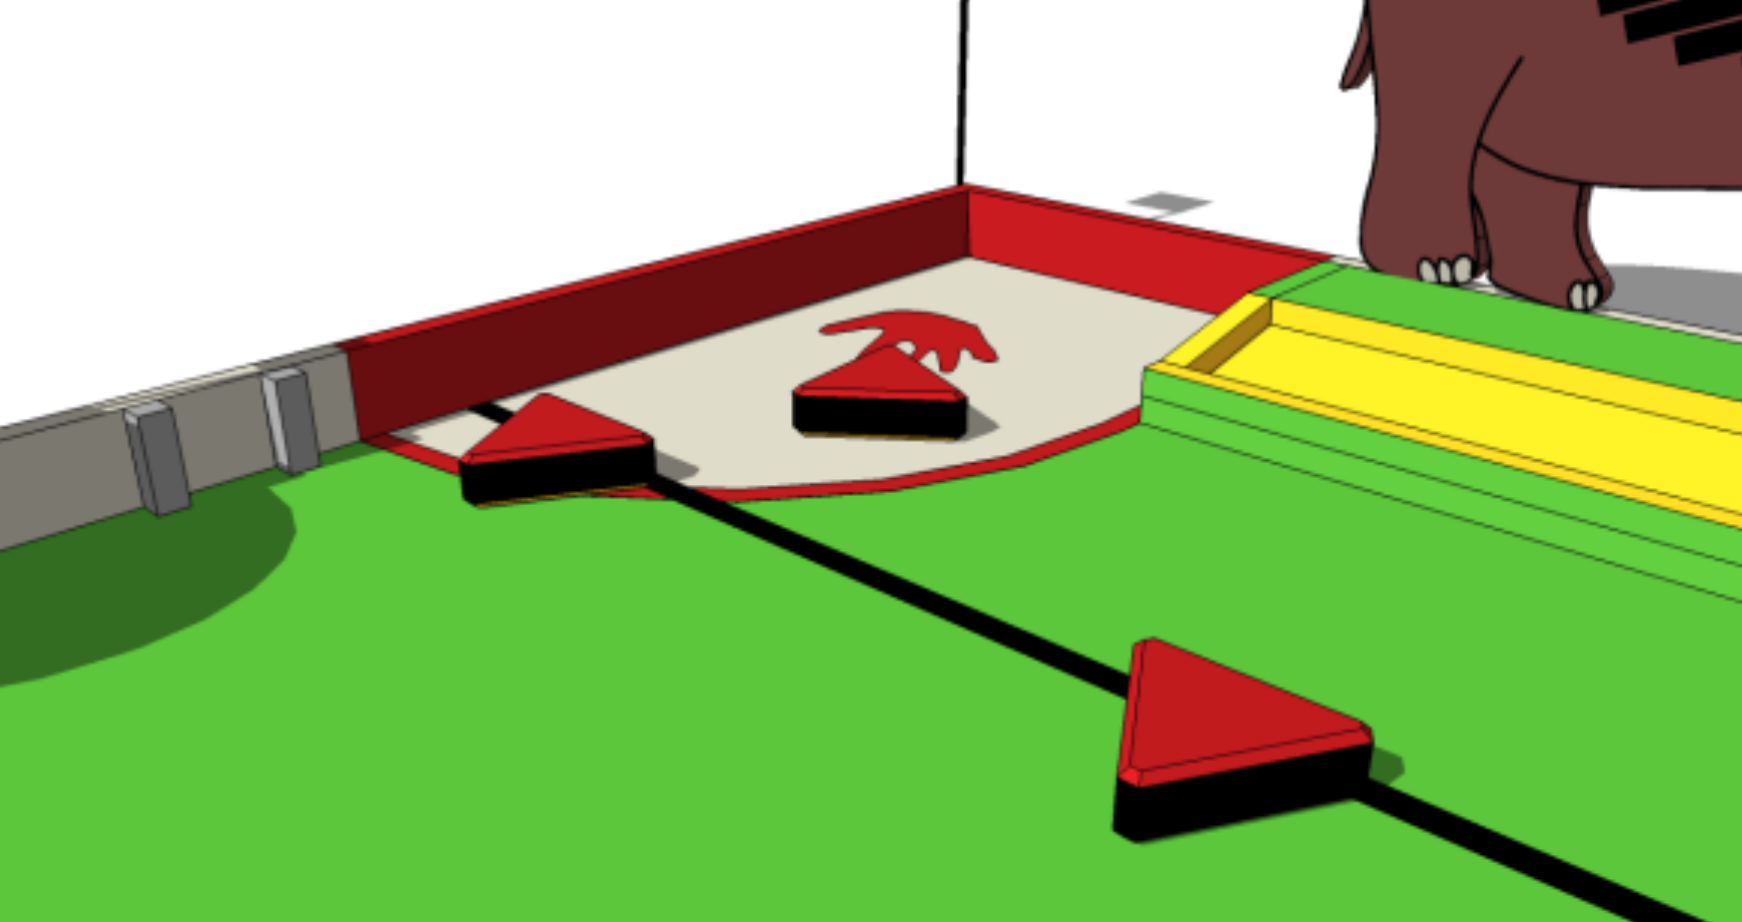
\includegraphics[height=3cm]{content/image/1_fire_1}       
					\end{subfigure}
					\begin{subfigure}[b]{0.49\textwidth}
						\centering
						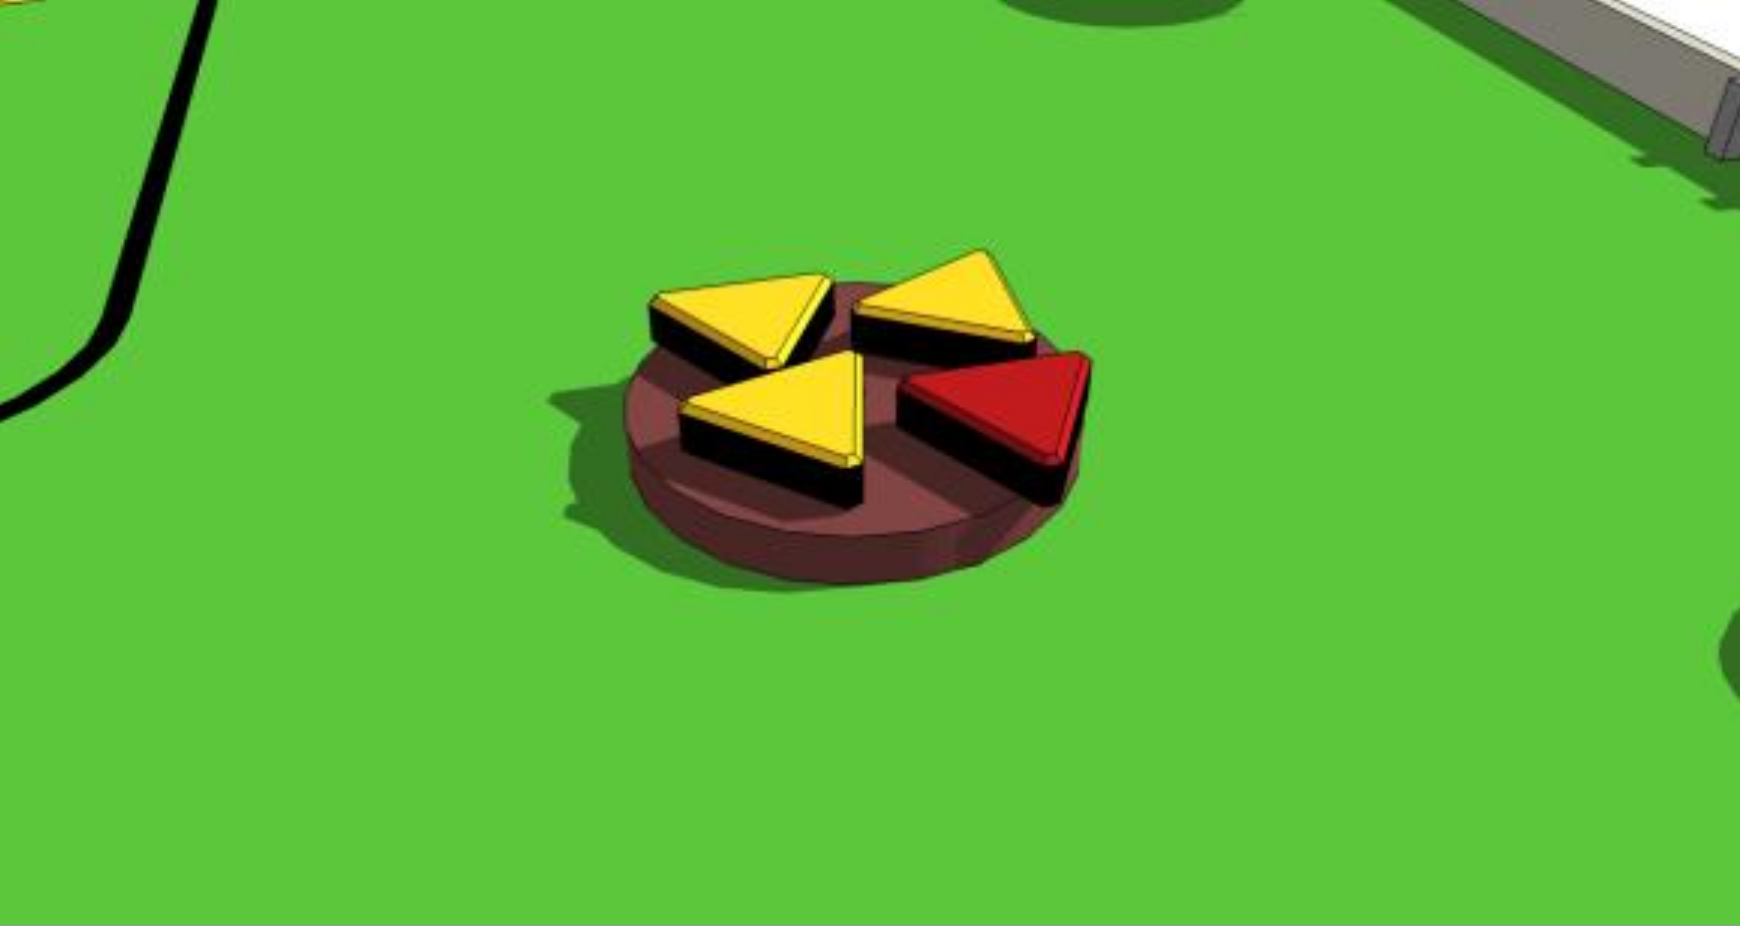
\includegraphics[height=3cm]{content/image/1_fire_2}         
					\end{subfigure}
					\caption[\gls{g:fresko}]{\gls{g:fresko} \cite{pic:eurobot_spielfeld}}
					\label{abb:fire}
		    	\end{figure}
		    	%
				\item[Fr�chte sammeln (\gls{g:fruits})] Auf dem Spielfeld sind insgesamt gesamt vier B�ume verteilt (siehe Abbildung \ref{abb:spielfeld_eurobot}), die jeweils mit 6 Fr�chten (5 gesunde, eine vergiftet) best�ckt sind. Aufgabe ist es die Fr�chte zu ernten, die giftigen auszusortieren und die restlichen im korrekten Beh�ltnis (Mannschaftsfarbe) zu deponieren. Punkte geben korrekt platzierte und gesunde Fr�chte. Die Abbildung \ref{abb:fruits} zeigt die beiden Bestandteile Baum und Beh�ltnis. 
				\begin{figure}[htbp] %htbp
					\centering
					\begin{subfigure}[b]{0.49\textwidth}
						\centering
						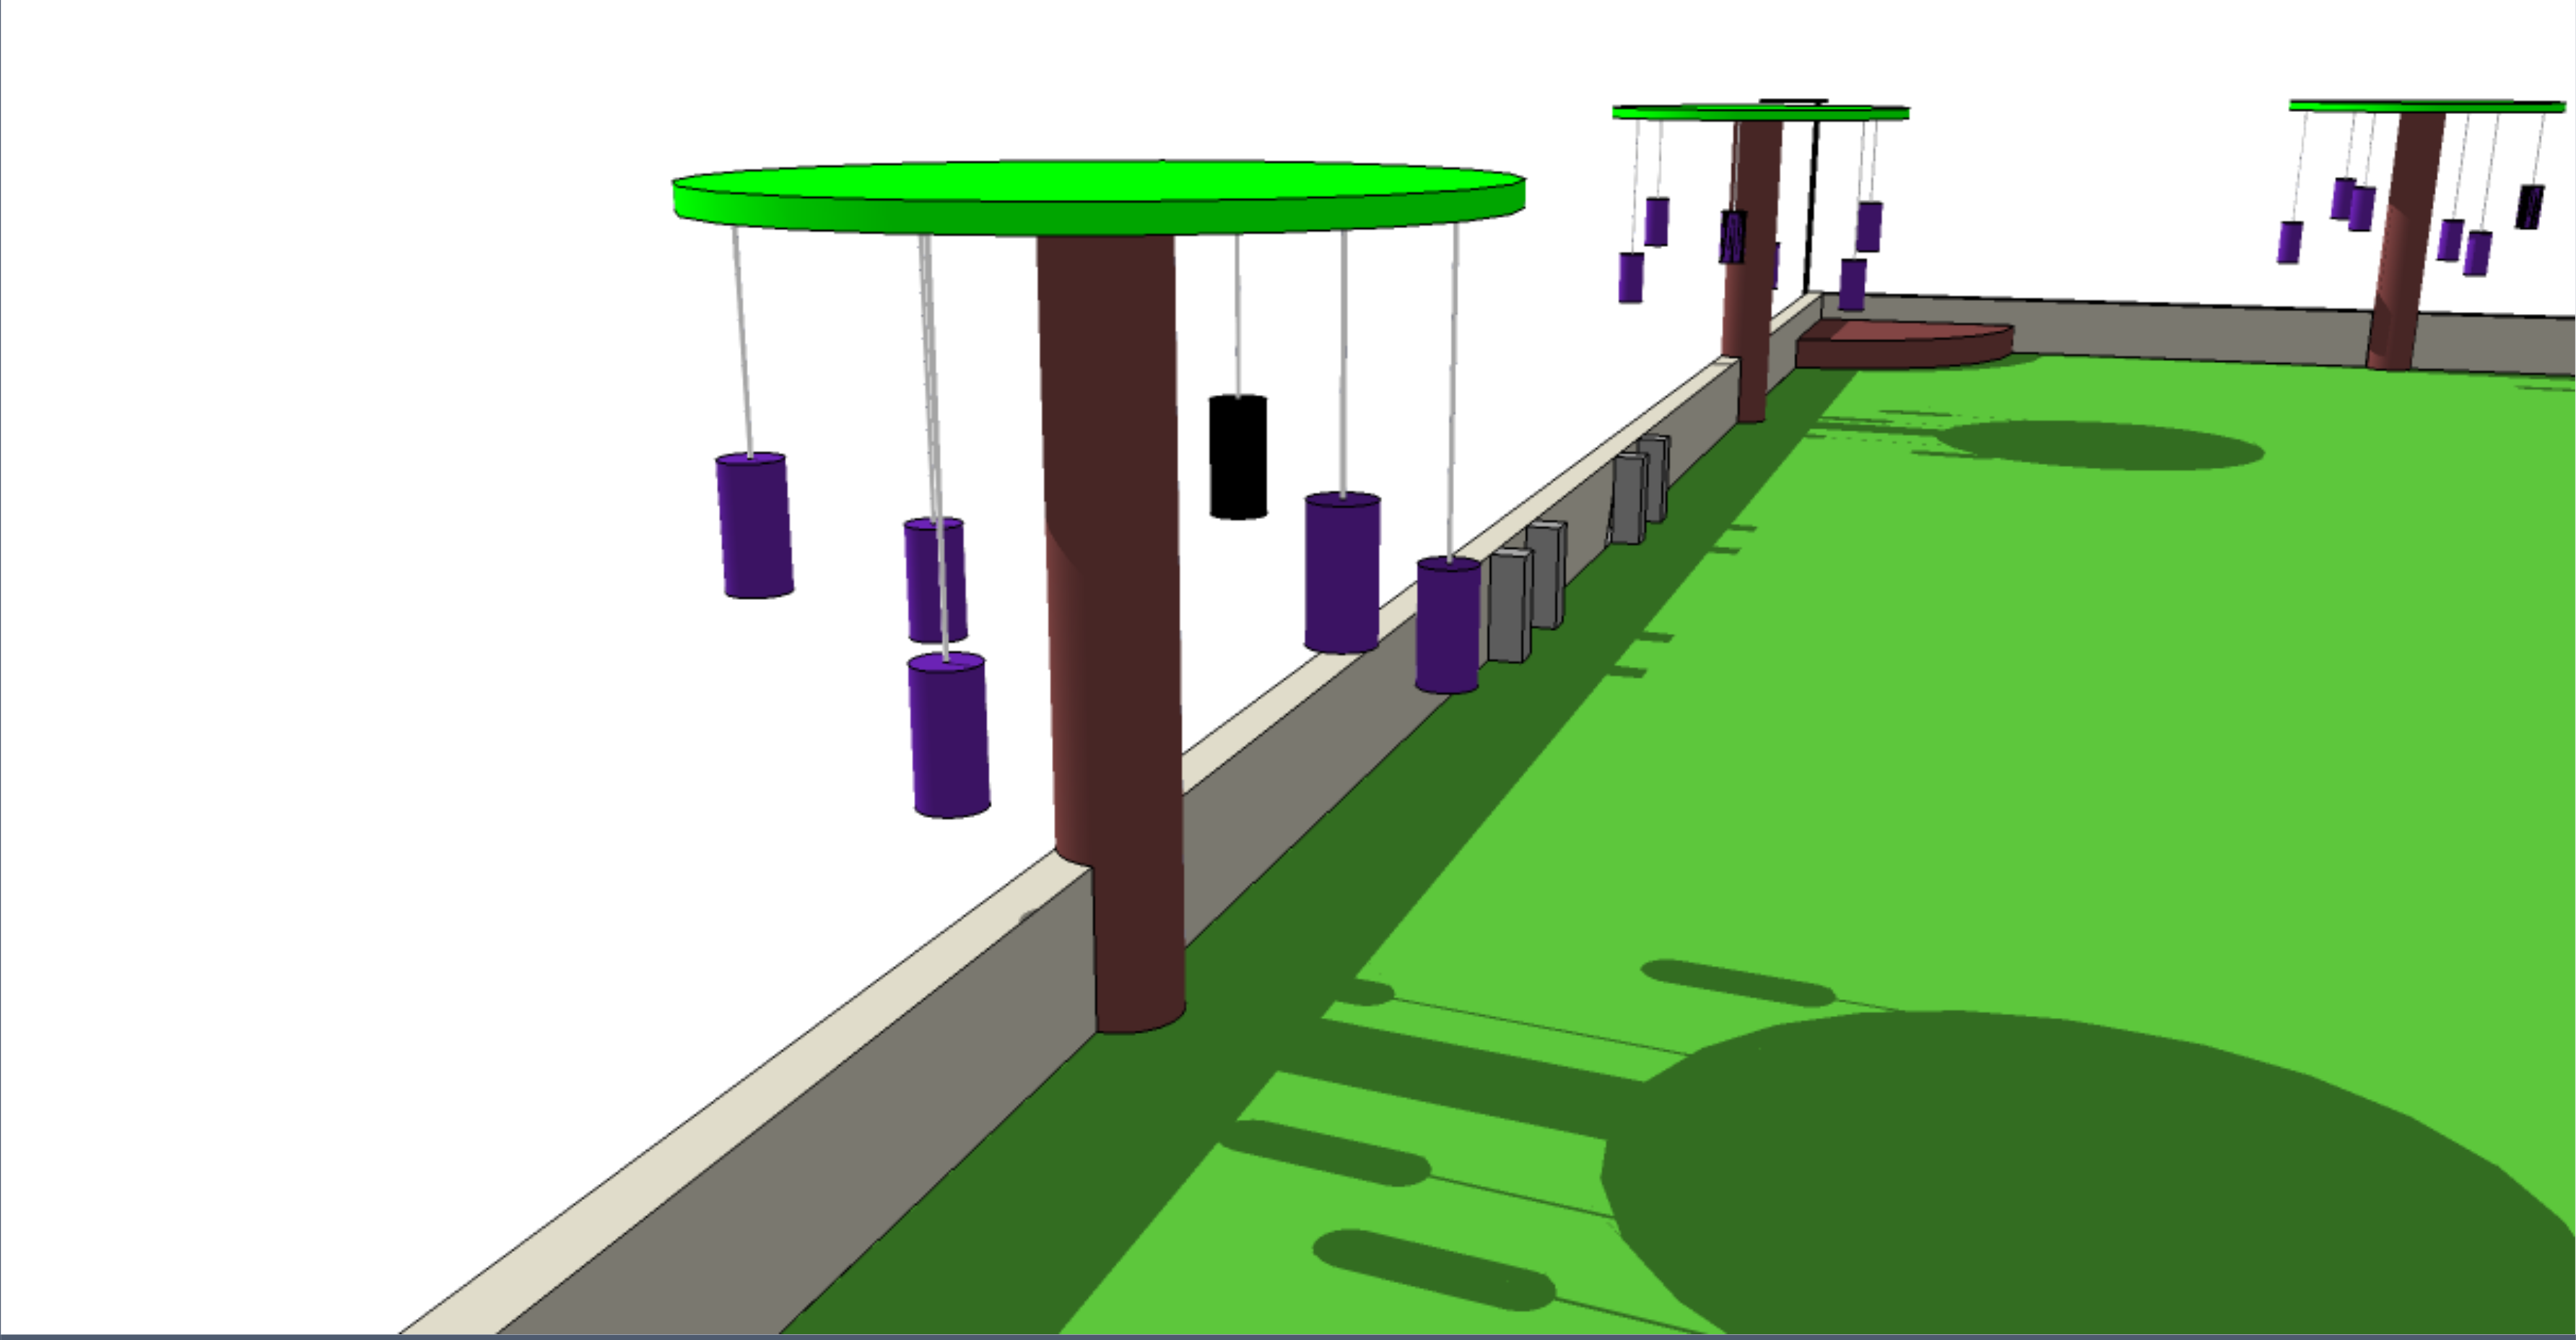
\includegraphics[height=3cm]{content/image/1_fruits_1}       
					\end{subfigure}
					\begin{subfigure}[b]{0.49\textwidth}
						\centering
						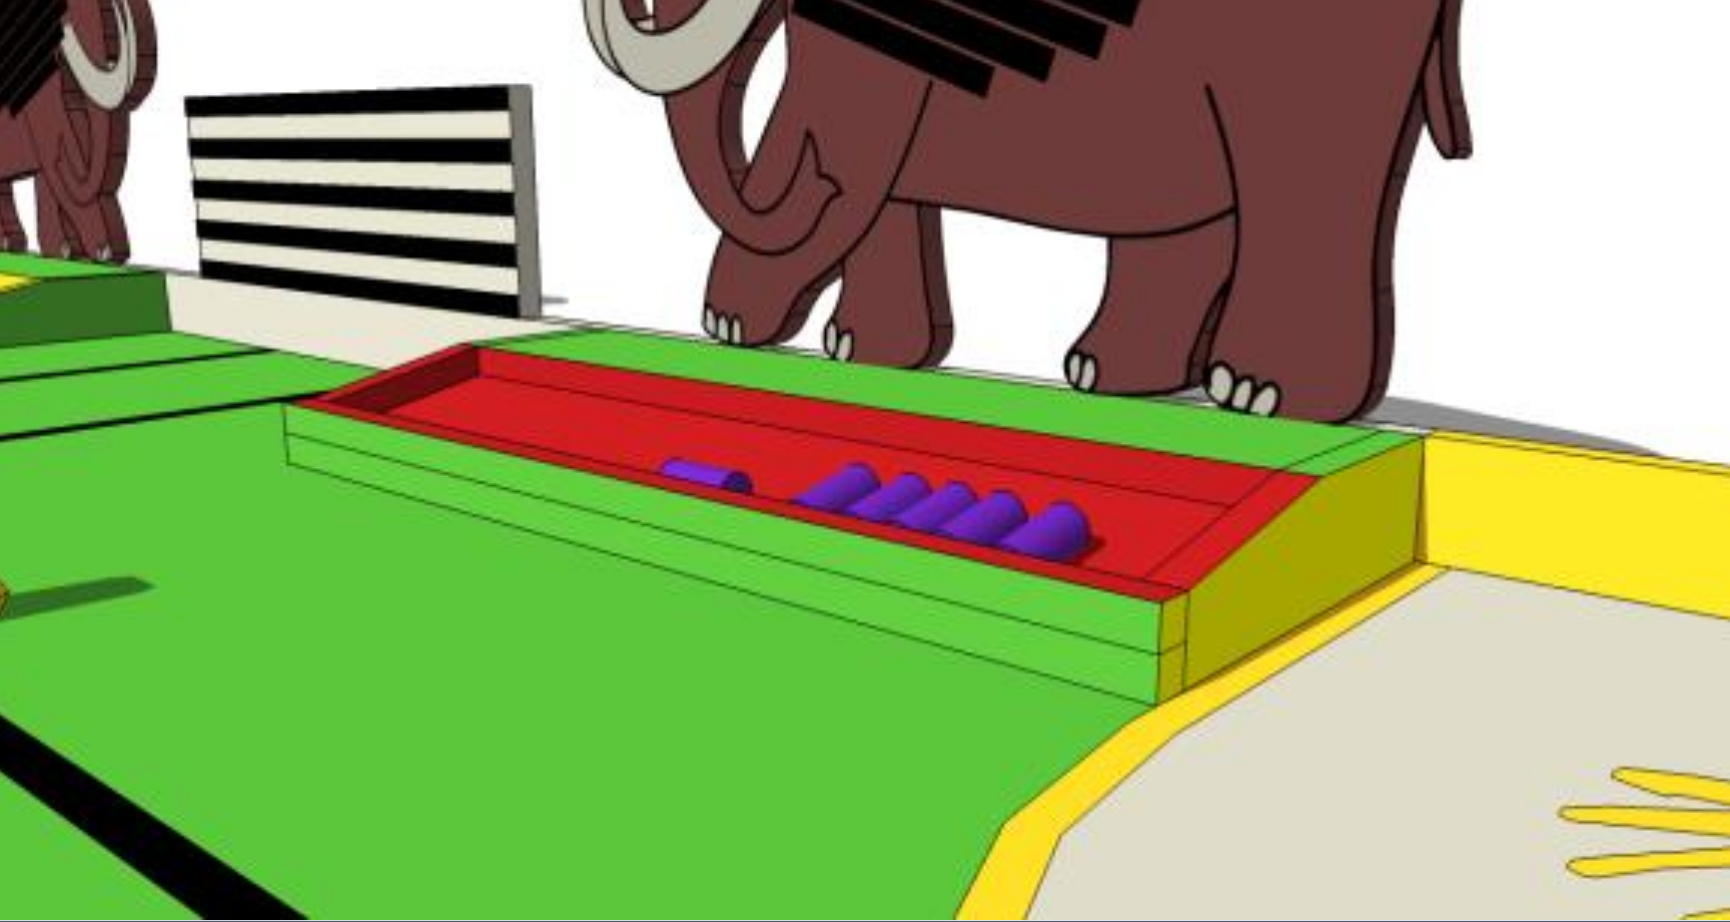
\includegraphics[height=3cm]{content/image/1_fruits_2}         
					\end{subfigure}
					\caption[\gls{g:fruits}]{\gls{g:fruits} \cite{pic:eurobot_spielfeld}}
					\label{abb:fruits}
		    	\end{figure}
		    	%
		    	\newpage
				\item[Mammut jagen (\gls{g:mammut})] Die beiden vorhanden Mammuts weisen beide \gls{g:velcro}-Streifen auf. Diese dienen dazu abgefeuerte B�lle der Roboter aufzufangen (B�lle sind auch mit \gls{g:velcro} versehen). Die als Speer dienenden B�lle werden vor dem eigentlichen Spiel in einem Roboter gespeichert und sind sechs an der Zahl. Beide Mammuts d�rfen von beiden Mannschaften abgeschossen werden, wobei unter bestimmten Umst�nden Zusatzpunkte erzielt werden k�nnen \cite[S.14]{lit:eurobot}. Punkte geben nur B�lle, die an den Mammuts haften bleiben. Die Abbildung \ref{abb:mammut} zeigt zwei abgeschossene Mammuts.
				\image{content/image/1_mammut}{scale=0.5}{htbp}[\gls{g:mammut} \cite{pic:eurobot_spielfeld}][\gls{g:mammut}][abb:mammut]
				%
				\item[Mammut fangen (\gls{g:mammut_catch})] Bei der Aufgabe \gls{g:mammut_catch} handelt es sich um eine Zusatzaufgabe (Funny Action). Ziel ist es ein Netz �ber eines der vorhandenen Mammuts zu werfen. F�r das erhalten von Punkten ist Bedingung, dass das Netz auf dem Mammut liegen bleibt. Die Aufgabe wird nicht w�hrend der eigentlichen Spielrunde durchgef�hrt, sonder am Schluss innerhalb einer zur Verf�gung gestellter Zusatzzeit.
			\end{description}
		%
		%
		\subsection{Spielfeld}\label{ss:spielfeld}
			Alle Spielaufgaben werden auf einem vorgegeben Spielfeld ausgetragen. Das Feld weist folgende Eigenschaften auf:
			\begin{itemize}
				\item Dimension 3x2 Meter
				\item Zwei Startbereiche (rote und gelbe Hand)
				\item M�glichkeit zum Platzieren von bis zu 3 Beacons pro Mannschaft am Rande des Speilfeldes
				\item Fixe Startpositionen der einzelnen Spielelemente (Ausnahme: Beeren an den B�umen)
			\end{itemize}
			\newpage
			Alle Farben sowie Dimensionen der Spielelemente sind durch das Reglement vorgegeben \cite[S.32]{lit:eurobot}. Das genaue Aussehen des Spielfeldes ist der Abbildung \ref{abb:spielfeld} zu entnehmen.\par
			%
			Die Herstellungen eines regelkonformen Tisches ist eine Zusatzaufgabe des Teams und muss parallel zu den eigentlichen Aufgaben erledigt werden\footnote{Im Zuge der Fertigung wurde ein zusammenfassender Bericht erstellt, der gemachte Erfahrungen aufzeigen soll. Das Dokument ist auf dem Netzlaufwerk hinterlegt: \path{\\boiler.bfh.ch\data\public\projects\Eurobot\2014\20_Kernteam\23_Dokumentation\Tisch_Herstellung_2014.docx}}.  
			\image{content/image/1_spielfeldnavigation}{scale=.7}{htbp}[Spielfeld \cite{pic:eurobot_spielfeld}][Spielfeld][abb:spielfeld]
	%
	%
	% Motivation
	\section{Motivation}\label{s:motivation}
		Die Realisierung eines Roboters in einem Team und die Teilnahme an einem internationalen Wettbewerb an sich beinhaltet ist schon Motivation genug. Weiter kommen die Punkte Mannschaftszugeh�rigkeit und die M�glichkeit etwas von Grunde heraus selber zu entwickeln hinzu. Hinsichtlich des sp�teren Berufslebens bietet es zudem Einblick in eine gr�sser angelegte Projektarbeit, in der abteilungs�bergreifend gemeinsam an einem Problem gearbeitet wird.\par 
		%
		Dieses Jahr ist so weit noch speziell, da die nationale Ausscheidung in Burgdorf stattfinden wird und somit unsere Mannschaft Heimvorteil geniesst. Nat�rlich geht damit auch ein gewisser Druck einher, m�glichst eine gute Platzierung zu erreichen. Wobei dieser Druck auch ein weiterer Motivationsfaktor ist.
	%
	%
	% Zieldefinition
	\section{Zieldefinition}\label{s:zieldefinition}
		Dadurch das die Spielaufgaben erst nach der Fertigstellung des Pflichtenhefts\footnote{siehe Anhang A\textit{Pflichtenheft}}bekannt wurden und viele Ziele direkt von ihnen abh�ngig sind, werden folgend weiterf�hrende und erg�nzende Ziele der \gls{ac:pa1} (Teile betreffen auch die \gls{ac:pa2}) definiert.
		%
		%
		\subsection{Spielstrategie}\label{ss:spielstrategie}
			Die Spielstrategie ist einer der zentralen Aufgaben des \gls{ac:kernteam}s. Sie entscheidet sp�ter �ber Erfolg oder Misserfolg am Wettbewerb. Um m�glichst dynamisch auf das Verhalten des Gegners reagieren zu k�nnen, m�ssen m�gliche Szenarien erstellt und analysiert werden. Dabei soll zwischen einer optimalen und einer backup Strategie unterschieden werden.
			\begin{description}
				\item[Optimale Strategie] Wenn immer m�glich soll die optimale Strategie verfolgt werden. Sie hat zum Ziel m�glichst die maximale Punktzahl mit den gegebenen M�glichkeiten zu erreichen.
				\item[Backup Strategie] Sollte es w�hrend der Umsetzungsphase zu unvorhersehbaren Problemen kommen, muss eine Alternative zur optimalen Strategie vorhanden sein. Sie soll jedoch nur im �ussersten  Notfall zu Zuge kommen und gleichwohl zur Teilnahme beim Wettbewerb berechtigen.
			\end{description}
			%
			Im Abschnitt \ref{s:strategie} \textit{Strategie} ab Seite \pageref{s:strategie} wird die Erarbeitung der Strategien erl�utert.
		%
		%
		\subsection{Testkonzept}\label{ss:testkonzept}
			Wichtig f�r das Validieren der Umsetzungen sind vordefinierte Testszenarien. Zum einen kann damit im Bereich Projektmanagement\footnote{siehe Abschnitt \ref{ch:projektmanagement} \textit{Projektmanagement} ab Seite \pageref{ch:projektmanagement}} den Fortschritt des Projekts validiert und zum anderen Probleme festgestellt und behoben werden.\par 
			%
			\newpage
			Jeder Teilbereich des Roboters bekommt einer eigene Testreihe zugeordnet. Dabei ist jedes Teilteam f�r das Testen der erstellten L�sungen selber verantwortlich. Bez�glich des \gls{ac:kernteam}s m�ssen folgende Bereich abgedeckt werden.
			\begin{itemize}
				\item Die definierten Kommunikationsprotokolle und deren Umsetzung in Software
				\item Peripherien der Spielmanipulation 
				\item Umsetzung der Spielstrategie
			\end{itemize}
			%
			Die Tests sollen in einem ersten Schritt (falls m�glich) unabh�ngig von anderen Komponenten durchgef�hrt werden. Abschliessend werden Tests im Verbund des Roboters folgen (siehe Anhang E \textit{Funktionstests Testprotokolle PA2}).
		%
		%
		\subsection{Kommunikation}\label{ss:kommunikation}
			Die Kommunikation gliedert sich in die Bereiche intern und extern. Die interne Kommunikation dient dem Austausch von Daten zwischen den einzelnen Roboter-Komponenten. Die externe Kommunikation beinhaltet den Austausch von Datens�tzen zwischen den beiden Robotern.\par  
			%
			Im Zuge der \gls{ac:pa1} sollen entsprechende Protokolle definiert und umgesetzt werden. Die Realisierung soll so erfolgen, dass die �brigen Teilteams durch die Implementierung nicht belastetet werden und den gebotenen Funktionsumfang einfach nutzen k�nnen. Die Kommunikation soll gen�gend Kapazit�ten f�r Erweiterungen offen halten und m�glichst sicher erfolgen.\par 
			%
			In den Abschnitten \ref{ss:cangatekeeper} \textit{CANGatekeeper}, \ref{ss:Control_area_network} \textit{Control Area Network} und \ref{s:kommunikation} \textit{Kommunikation} wird die Definition und Implementierung aufgezeigt. 
		%
		%
		\subsection{Mechanik}\label{ss:mechanik}
			Hauptaugenmerk der \gls{ac:pa1} liegt auf dem Fertigstellen des kleinen Roboters, der die Aufgaben \gls{g:fresko} und \gls{g:mammut} erf�llen soll. Dabei soll die Mechanik m�glichst einfach und solide konstruiert sein. Ebenfalls soll die Anzahl der n�tigen Aktoren auf ein Minimum reduziert werden.
%
%Kapitel 2: Projektmanagement
%%%%%%%%%%%%%%%%%%%%%%%%%%%%%%%%%%%%%%%%%%%%%%%%%%%%%%%%%%%%%%%%%%%%%%%%%%%%%%%
% Titel:   Projektmanagement
% Autor:   meert1
% Datum:   05.01.2014
% Version: 0.2.0
%%%%%%%%%%%%%%%%%%%%%%%%%%%%%%%%%%%%%%%%%%%%%%%%%%%%%%%%%%%%%%%%%%%%%%%%%%%%%%%
%
%:::Change-Log:::
% Versionierung erfolgt auf folgende Gegebenheiten: -1. Release Versionen
%                                                   -2. Neue Kapitel
%                                                   -3. Fehlerkorrekturen
%
% 0.2.0       Erstellung der Kapitel und Unterkapitel
% 0.0.1       Erstellung der Datei
%%%%%%%%%%%%%%%%%%%%%%%%%%%%%%%%%%%%%%%%%%%%%%%%%%%%%%%%%%%%%%%%%%%%%%%%%%%%%%%    
\chapter{Projektmanagement}\label{ch:projektmanagement}
	\section{Ressourcen}\label{s:ressourcen}
	   Das Projekt wird in mehrere Teilgruppen aufgeteilt\footnote{F�r detaillierte Informationen siehe Abschnitt \ref{ss:team}}. Jeder dieser Teilgruppen bekommt eine spezifische Aufgabe zugewiesen, womit ein effizientes Arbeiten sichergestellt werden kann. Dem Gesamtteam �bergeordnet ist die administrative Projektleitung, die zum einen eine beratende und zum anderen eine kommunikative\footnote{Abteilungs�bergreifend zwischen den beteiligten Dozenten} Funktion einnimmt. Fachlich unterst�tzt wird das Team von einem Fachausschuss, bestehend aus den betreuenden Dozenten.\par 
		%
		\subsection{Team}\label{ss:team}
		    Das Gesamtteam besteht aus 12 Personen (8 Elektroabteilung, 4 Mechanikabteilung), die in insgesamt f�nf Teilteams aufgeteilt sind. Die genau Aufteilung sind in der Tabelle \ref{tab:gesamtteam} zu finden.\par
		    %
		    \begin{table}[htbp]
		        \centering
		        \begin{tabular}{|l|l|l|l|l|l|} 
		            \hline
		            \rowcolor{bfhblue}
		            \textcolor{white}{Name} & \textcolor{white}{Vorname} & \textcolor{white}{K�rzel} & \textcolor{white}{E-Mail} & \textcolor{white}{Klasse} & \textcolor{white}{Team}\\
		            \hline
		            Grossenbacher & Simon & gross10 & \href{mailto: gross10@bfh.ch}{gross10@bfh.ch} & E3b & Kernteam\\
		            \hline
		            Meerstetter & Tobias & meert1 & \href{mailto: meert1@bfh.ch}{meert1@bfh.ch} & E3b & Kernteam\\
		            \hline
		            Rohrbach & Patrick & rohrp1 & \href{mailto: rohrp1@bfh.ch}{rohrp1@bfh.ch} & M3a & Kernteam\\
		            \hline
		            Roth & Hannes & rothh3 & \href{mailto: rothh3@bfh.ch}{rothh3@bfh.ch} & M3a & Kernteam\\
		            \hline
		            Balz & Kilian & balzk1 & \href{mailto: balzk1@bfh.ch}{balzk1@bfh.ch} & M3a & Antrieb\\
		            \hline
		            Haldemann & Jascha & haldj3 & \href{mailto: haldj3@bfh.ch}{haldj3@bfh.ch} & E3a & Antrieb\\
		            \hline
		            Heimsch & Gunnar & heimg1 & \href{mailto: heimg1@bfh.ch}{heimg1@bfh.ch} & E3b & Navigation\\
		            \hline
		            Plattner & Simon & plats1 & \href{mailto: plats1@bfh.ch}{plats1@bfh.ch} & E3a & Navigation\\
		            \hline
		            Zurschmiede & Reto & zursr1 & \href{mailto: zursr1@bfh.ch}{zursr1@bfh.ch} & E3a & Navigation\\
		            \hline
		            K�ser & Nicola & kasen1 & \href{mailto: kasen1@bfh.ch}{kasen1@bfh.ch} & E3a & Naherkennung\\
		            \hline
		            Greiler & Roland & greir1 & \href{mailto: greir1@bfh.ch}{greir1@bfh.ch} & M3a & Verdrahtung-/Volumen\\
		            \hline
		            Reust & Ralph & reusr6 & \href{mailto: reusr6@bfh.ch}{reusr6@bfh.ch} & M3a & Verdrahtung-/Volumen\\
		            \hline
		        \end{tabular}
		        \caption{�bersicht Eurobotteam}
		        \label{tab:gesamtteam}  
		    \end{table}
		    %
		    Die einzelnen Aufgaben der Teilteams setzen sich wie folgt zusammen:
		    %
			\begin{description}
			    \item[\acrfull{ac:kernteam}] Das \gls{ac:kernteam} �bernimmt das Projektmanagement und die Koordination des Projekts. Weiter ist es zust�ndig f�r die Fertigstellung eines lauff�higen Roboters am Ende der \gls{ac:pa1}. Dies beinhaltet ebenfalls die Werkzeuge zur Spielmanipulation.
			    \item[\gls{ac:navigationsteam}] Das \gls{ac:navigationsteam} teilt sich in drei Bereiche: Ultraschall- und Lasernavigation, sowie Kalmannfilter. Ziel ist die Realisierung einer zuverl�ssigen und genauen Navigationseinheit.
			    \item[\gls{ac:antriebsteam}] Der Antrieb wird vom Vorjahresteam �bernommen, wird durch das \gls{ac:antriebsteam} aber noch verfeinert. Zus�tzlich werden erweiterte Regelm�glichkeiten implementiert.
			    \item[\gls{ac:volumenteam}] Das \gls{ac:volumenteam} erarbeitet ein entsprechendes Konzept und setzt dieses anschliessend um.
			    \item[\gls{ac:naherkennungsteam}] Die Naherkennung muss Objekte in unmittelbarer Umgebung des Roboters zuverl�ssig erkennen. Ziel dieses Team ist es, eine Kollision mit dem Gegner verhindern zu k�nnen.
			\end{description}
			%
			Jedes dieser Teilteams organisiert sich weitestgehend selber, ist aber �ber die gesamte Projektdauer in enger Verbindung zu den �brigen Arbeitsgruppen.
		%
		\subsection{Projektleitung}\label{ss:projektleitung}
		Die Projektleitung besteht aus einer Person (n�here Information dazu in Tabelle \ref{tab:projektleitung}). Sie �bernimmt administrative Aufgaben wie das Verwalten von externen Bestellungen und Austausch von wichtigen Informationen zwischen der Elektro- und Maschinentechnikabteilung. Weiter ber�t sie das Gesamtteam bei anstehenden Problemen und hilft bei der L�sungsfindung.
		    %    
		\begin{table}[htbp]
		\centering
		\begin{tabular}{|l|l|l|l|l|l|} 
		    \hline
		    \rowcolor{bfhblue}
		    \textcolor{white}{Name} & \textcolor{white}{Vorname} & \textcolor{white}{K�rzel} & \textcolor{white}{E-Mail}\\
		    \hline
		    Schmutz & Reto & sur7 & \href{mailto: sur7@bfh.ch}{sur7@bfh.ch}\\
		    \hline
		\end{tabular}
		\caption{Zusammenstellung Projektleitung}
		\label{tab:projektleitung}  
		\end{table}
		%
		\newpage
		\subsection{Fachausschuss}\label{ss:fachausschuss}
		Der Fachausschuss setzt sich aus den betreuenden Dozenten zusammen. Jedes Teilteam bekommt einen oder mehrere Dozenten zugeteilt, die in beratender Funktion zur Seite stehen. Die Zuteilung richtet sich nach den jeweiligen Aufgaben und den Fachgebieten der Dozenten. Durch die enge Betreuung sollen Fehler und Probleme schneller erkannt und behoben werden. Angaben zu den Dozenten sind in der Tabelle \ref{tab:fachausschuss} zu finden.
		    %
		\begin{table}[H]
		  \centering
		  \begin{tabular}{|l|l|l|l|l|l|} 
		      \hline
		      \rowcolor{bfhblue}
		      \textcolor{white}{Name} & \textcolor{white}{Vorname} & \textcolor{white}{K�rzel} & \textcolor{white}{E-Mail} & \textcolor{white}{Team}\\
		      \hline
		      Brun & Roland & brr1 & \href{mailto: roland.brun@bfh.ch}{roland.brun@bfh.ch} & \gls{ac:volumenteam} \\
		      \hline
		      G�ller & Walter & glw1 & \href{mailto: walter.gueller@bfh.ch}{walter.gueller@bfh.ch} & \gls{ac:kernteam}, \gls{ac:volumenteam}\\
		      \hline
		      Hungerb�hler & Roland & hlr2 & \href{mailto: roland.hungerbuehler@bfh.ch}{roland.hungerbuehler@bfh.ch} & \gls{ac:antriebsteam}\\
		      \hline
		      Kucera & Martin & kem4 & \href{mailto: martin.kucera@bfh.ch}{martin.kucera@bfh.ch} & \gls{ac:naherkennungsteam}\\
		      \hline
		      Lanz & Daniel & lad1 & \href{mailto: daniel.lanz@bfh.ch}{daniel.lanz@bfh.ch} & \gls{ac:kernteam}\\
		      \hline
		      Oesch & Ivo & osi1 & \href{mailto: ivo.oesch@bfh.ch}{ivo.oesch@bfh.ch} & \gls{ac:kernteam}, \gls{ac:antriebsteam}, \gls{ac:navigationsteam}\\
		      \hline
		      Vetter & Rolf & vtr1 & \href{mailto: rolf.vetter@bfh.ch}{rolf.vetter@bfh.ch} & \gls{ac:navigationsteam}\\
		      \hline
		      Wandel & Jasmin & wdj1 & \href{mailto: jasmin.wandel@bfh.ch}{jasmin.wandel@bfh.ch} & \gls{ac:navigationsteam}\\
		      \hline
		      Weber & Roger & wbr1 & \href{mailto: roger.weber@bfh.ch}{roger.weber@bfh.ch} & Software alg.\\
		      \hline
		  \end{tabular}
		  \caption{Zusammenstellung Projektleitung}
		  \label{tab:fachausschuss}  
		\end{table}
	%
	\section{Projektplanung}\label{s:projektplanung}
	Zu Beginn der Projektarbeit musste vor allem viel f�r die \gls{ac:pa1} geplant werden. Da nicht von Anfang an bekannt war, welches die genauen Aufgaben f�r den Wettbewerb sind, wurde zuerst ein grober Ablauf des Projektes Erarbeitet.\par
	%
	Nach der Bekanntgabe der Regeln wurde schliesslich ein Zeitplan �ber die ganze \gls{ac:pa1} gemacht, um auch die erwarteten Ergebnisse �berpr�fen zu k�nnen. Dazu jedoch mehr im Kapitel \ref{s:controlling} \textit{Controlling} auf Seite \pageref{s:controlling}.
		%
		\subsection{Projektablauf}\label{ss:projektablauf}
		Der Projektablaufplan in Abbildung \ref{abb:ablaufdiagramm} auf Seite \pageref{abb:ablaufdiagramm} zeigt systematisch den groben Ablauf des Projektes. Grunds�tzlich wurde der Ablauf in f�nf Phasen unterteilt, welche jeweils die entsprechenden T�tigkeiten der Phase enthalten. 
		\image{content/image/2_ablaufdiagramm}{scale=1}{htbp}[Ablaufdiagramm][abb:ablaufdiagramm]
		%
		\subsection{Zeitplanung}\label{ss:Zeitplanung}
		Der Zeitplan in Abbildung \ref{abb:zeitplan} auf Seite \pageref{abb:zeitplan} wurde in drei Teile unterteilt:
		%
		\begin{description}
			\item[Meilensteine Eurobot] Die Meilensteine f�r das gesamte Eurobot Team wurden in dieser Kategorie angelegt, da diese auch f�r die anderen Teams wichtige Meilensteine sind.
			%
			\item[Allgemein] In diesem Abschnitt werden allgemeine T�tigkeiten f�r das Eurobot Team definiert. In diese Kategorie fallen z.B. das Tisch- und Spielelementbebauen hinein.
			%
			\item[Kernteam] Im Abschnitt Kernteam werden die Meilensteine, so wie die T�tigkeiten des Kernteams selbst fest gehalten. 
		\end{description}
		%
		Die Eurobot Meilensteine, die allgemeinen T�tigkeiten und die Meilensteine des Kernteams wurden bereits fr�h kommuniziert. Die anderen Teams konnten mit Hilfe dieser Zeiten ihre Zeitplanung erstellen oder gegebenen falls anpassen, da manche Termine des Kernteams auch wesentliche Einfl�sse oder Forderungen an die anderen Teams mit sich f�hren. 
		%
		\image{content/image/2_Zeitplanung}{scale=1, angle=90}{htbp}[Zeitplanung Kernteam][abb:zeitplan]
		%
		\subsubsection{Ist-Aufnahme}\label{sss:istaufnahme}
		Grunds�tzlich wurden die meisten Arbeiten p�nktlich fertig gestellt. Gegen Ende der \gls{ac:pa1} ergaben sich gewisse Verz�gerungen, da die mechanischen Teilsysteme nicht termingerecht fertig gestellt werden konnten. Dies hatte auch Auswirkungen auf die Implementierung der Aufgabenl�sung in der Software. Im Kapitel \ref{s:weiteres_vorgehen} \textit{Weiteres Vorgehen} auf Seite \pageref{s:weiteres_vorgehen} sind die ausstehenden Arbeiten aufgelistet. 
	%
	\section{Koordination}\label{s:koordination}
	F�r die Koordination eines Teilprojektes sind die in Tabelle \ref{tab:gesamtteam} auf Seite \pageref{tab:gesamtteam} auflisteten Personen jeweils zust�ndig. Innerhalb des Kernteams wurde haupts�chlich zwischen Mechanik und Elektronik unterschieden, damit klarer ist, wer f�r welche Arbeiten verantwortlich ist. Zus�tzlich hat eine Person aus dem Kernteam die Aufgabe des Controlling des gesamten Eurobotteams �bernommen. Dazu jedoch mehr im folgenden Kapitel auf Seite \pageref{s:controlling}.\par
	%
	Als Unterst�tzung f�r die Koordination der Teams Stehen die Projektleitung\footnote{Namentlich Reto Schmutz - Mehr da zu auf Seite \pageref{ss:projektleitung} Projektleitung} und der Fachausschuss\footnote{Weitere Informationen im Kapitel \ref{ss:fachausschuss} \textit{Fachausschuss} auf Seite \pageref{ss:fachausschuss}  } jeder zeit mit Rat und Tat zur Verf�gung.
	%
	\section{Controlling}\label{s:controlling}
	Zur �berwachung des Projektablaufs wurden nebst den R�ckmeldungen der anderen Teams auch noch drei Kontrollmittel definiert, mit denen ein m�glichst reibungsloser Ablauf der \gls{ac:pa1} gew�hrleistet werden soll. Da die Aufgabe des Projektcontrolling vom Kernteam �bernommen werden muss, kann dieser Task lediglich teil zeitlich erledigt werden. \par
	%
	Es wurden folgende drei Kontrollmittel eingef�hrt:
	\begin{description}
		\item[Meilensteine] Jedes Team hatte zu Beginn des Projektes einen Zeitplan mit Meilensteine zu erstellen, die dem Kernteam abzugeben waren.
		%
		\item[Zwischenpr�sentation] In der Mitte der \gls{ac:pa1} hat jedes Team eine kleine Pr�sentation gehalten, in welcher die bereits erreichten und die noch zu erledigenden Arbeiten aufgezeigt wurden. Diese Pr�sentation diente so gleich als Wissensaustausch zwischen den einzelnen Teams. 
		%
		\item[Stand der Dinge] Gegen Ende der \gls{ac:pa1} hat jedes Team dem Kernteam ein Beschrieb des aktuellen Projektstandes eingereicht. Darin enthalten waren die erreichten Ziele und Meilensteine, so wie die noch ausstehenden Arbeiten, welche in der \gls{ac:pa2} fertig gemacht werden m�ssen.
	\end{description}
		%
		\subsection{Meilensteine}\label{ss:meilensteine}
		Die Meilensteine der anderen Teams wurden in ein Gesamtzeitplan eingef�gt, um jeder Zeit einen guten �berblick zu haben. Jeden Donnerstag konnte so mit jedem Team, welches einen Meilenstein ausstehend hatte, R�cksprache gehalten werden, um die Erreichung dieses zu �berpr�fen.  
		%
		\subsection{Zwischenpr�sentation}\label{ss:zwischenpr�sentation}
		Die Zwischenpr�sentation fand am Donnerstag dem 21.11.2013 statt. Dabei war das Ganze Team, Der Projektleiter und alle Dozenten, die das Eurobotteam betreuen. Anschliessend stand noch etwas Zeit f�r Fragen und Diskussionen zur Verf�gung.
		%
		\subsection{Stand der Dinge}\label{ss:stand_der_dinge}
		Mit den Informationen der Projektst�nde und den voraussichtlich auftretenden Aufgaben f�r den Bau des zweiten Roboters, konte das weitere Vorgehen geplant werden.
	%
	\section{Weiteres Vorgehen}\label{s:weiteres_vorgehen}
		Die noch verbleibenden Arbeiten der \gls{ac:pa1} gehen fliesend in die \gls{ac:pa2} �ber, in der auch der 2. Roboter gebaut wird. Dies bedeutet, dass die noch anstehenden Arbeiten aus der \gls{ac:pa1} eine Zusatzbelastung f�r die \gls{ac:pa2} darstellen. Ein grober Ablauf ist in der Abbildung \ref{abb:ablaufdiagramm_pa2} ersichtlich.\par
		\image{content/image/2_Ablaufdiagramm_PA2_Eurobot_2014_v1}{scale=.82}{htbp}[Ablaufdiagramm \gls{ac:pa2}][abb:ablaufdiagramm_pa2]
		%
		\newpage
		Durch den unterschiedlichen Fortschritt der einzelnen Teams werden einige Umstrukturierungen vorgenommen. In den Abschnitten \ref{ss:arbeiten_kernteam} bis \ref{ss:arbeiten_naherkennungsteam} ist dies dargestellt.\par
		%
		%Um eine sinnvolle Planung zu erm�glichen, wurde in diesem Abschnitt pro Team eine Auflistung der anstehenden Arbeiten f�r die \gls{ac:pa2} erstellt.
		%
		%\subsection{Umstrukturierung PA2}
		%
		\subsection{Arbeiten Kernteam}\label{ss:arbeiten_kernteam}
			\begin{table}[htbp]
			\centering
			\begin{tabular}{|l|l|l|l|l|l|} 
				 \hline
				 \rowcolor{bfhblue}
				 \textcolor{white}{Name} & \textcolor{white}{Vorname} & \textcolor{white}{K�rzel} & \textcolor{white}{Arbeit \%}\\
				 \hline
				 Grossenbacher & Simon & gross10 & 100\\
				 \hline
				 Haldemann & Jascha & haldj3 & 100\\
				 \hline
				 Rohrbach & Patrick & rohrp1 & 100\\
				 \hline
 				 Roth & Hannes & rothh3 & 100\\
 				 \hline
 				 Balz & Kilian & balzk1 & 50\\
				 \hline
			\end{tabular}
			\caption{Ressourcen Kernteam in \gls{ac:pa2}}
			\label{tab:ressourcen_kernteam_pa2}  
			\end{table}
			%
			\begin{description}
				\item[Aus \gls{ac:pa1}] Folgende Arbeiten stehen noch aus:
					\begin{itemize}
						\item Alle Funktionstest Roboter 1
						%
						\item Ball spicken und Bilder kleben zum laufen bringen
						%
						\item Strategie-Task schreiben
					%
					\end{itemize}
				%
				\item[F�r \gls{ac:pa2}] Neue dazu kommende Arbeiten:
					\begin{itemize}
						\item Netz werfen und Feueraufgabe
						%
						\item Strategie f�r zweiten Roboter
						%
						\item Naherkennung einbinden und Testen
						%
						\item Evtl. Bedienpanel entwerfen
						%
						\item Plakate und Teambeschreibung erstellen
						%
						\item Sponsoring
						%
						\item Ersatzteile f�r Wettbewerb organisieren 
					%
					\end{itemize}
			%
			\end{description}
			
		%
		\newpage
		\subsection{Arbeiten Navigationsteam} \label{ss:arbeiten_navigationsteam}
			\begin{table}[htbp]
			\centering
			\begin{tabular}{|l|l|l|l|l|l|} 
				 \hline
				 \rowcolor{bfhblue}
				 \textcolor{white}{Name} & \textcolor{white}{Vorname} & \textcolor{white}{K�rzel} & \textcolor{white}{Arbeit \%}\\
				 \hline
				 Heimsch & Gunnar & heimg1 & 100\\
				 \hline
				 Zurschmiede & Reto & zursr1 & 100\\
				 \hline
				 K�ser & Nicola & kasen1 & 80\\
				 \hline
			\end{tabular}
			\caption{Ressourcen Navigationsteam in \gls{ac:pa2}}
			\label{tab:ressourcen_navigationsteam_pa2}  
			\end{table}
			%
			\begin{description}
				\item[Aus \gls{ac:pa1}:] Folgende Arbeiten stehen noch aus
					\begin{itemize}
						\item Endg�ltiger Entscheid �ber Einsatz des Navigationssystems
					%
					\end{itemize}
				%
				\item[F�r \gls{ac:pa2}:] Neue dazu kommende Arbeiten
					\begin{itemize}
						\item Implementierung Kalman-Filter
						%
						\item Kommunikation zwischen Robotern
						%
						\item Evaluation des gekauften Ultraschallsystems
						%
						\item Design des gew�hlten Navigationssystems
						%
						\item Mechanik und Elektronik des Navigationssystems herstellen
						%
						\item Beacons - Funktion und Mechanik
					%
					\end{itemize}
			%
			\end{description}
		%
		\newpage
		\subsection{Arbeiten Antriebsteam} \label{ss:arbeiten_antriebsteam}
			\begin{table}[htbp]
			\centering
			\begin{tabular}{|l|l|l|l|l|l|} 
				 \hline
				 \rowcolor{bfhblue}
				 \textcolor{white}{Name} & \textcolor{white}{Vorname} & \textcolor{white}{K�rzel} & \textcolor{white}{Arbeit \%}\\
				 \hline
				 Plattner & Simon & plats1 & 100\\
				 \hline
				 Meerstetter & Tobias & meert1 & 100\\
				 \hline
				 Balz & Kilian & balzk1 & 50\\
				 \hline
			\end{tabular}
			\caption{Ressourcen Antriebsteam in \gls{ac:pa2}}
			\label{tab:ressourcen_antriebsteam_pa2}  
			\end{table}
			%
			%
			\begin{description}
				\item[Aus \gls{ac:pa1}:] Folgende Arbeiten stehen noch aus
					\begin{itemize}
						\item Strommessung
						%
						\item Drehzahlregelung Testen
						%
						\item Korrekte Ansteuerung der Motoren
						%
						\item Odometrie einlesen
					%
					\end{itemize}
				%
				\item[F�r \gls{ac:pa2}:] Neue dazu kommende Arbeiten
					\begin{itemize}
						\item Positionsregelung
						%
						\item Routenplanung
						%
						\item Antriebsmechanik Roboter 2
						%
						\item Testen
					%
					\end{itemize}
			%
			\end{description}
		%
		\subsection{Arbeiten Volumen- und Verdrahtungsteam} \label{ss:arbeiten_volumen_verdrahtung}
			\begin{table}[htbp]
			\centering
			\begin{tabular}{|l|l|l|l|l|l|} 
				 \hline
				 \rowcolor{bfhblue}
				 \textcolor{white}{Name} & \textcolor{white}{Vorname} & \textcolor{white}{K�rzel} & \textcolor{white}{Arbeit \%}\\
				 \hline
				 Greiler & Roland & greir1 & 100\\
				 \hline
				 Reust & Ralph & reusr6 & 100\\
				 \hline
			\end{tabular}
			\caption{Ressourcen Volumen- und Verdrahtungsteam in \gls{ac:pa2}}
			\label{tab:ressourcen_volumen_verdrahtung_pa2}  
			\end{table}
			%
			\begin{description}
				\item[Aus \gls{ac:pa1}:] Folgende Arbeiten stehen noch aus
					\begin{itemize}
						\item Verschalung des ersten Roboters 
						%
						\item Mechanik f�r Spielstartausl�sung
					%
					\end{itemize}
				%
				\item[F�r \gls{ac:pa2}:] Neue dazu kommende Arbeiten
					\begin{itemize}
						\item Volumenkonzept und Verkabelung Roboter 2
						%
						\item Testen und pr�fen der Speisung und Masse der beiden Roboter.
						%
						\item Gesamttest entwickeln und Gegnerroboter in Betrieb nehmen.
					%
					\end{itemize}
			%
			\end{description}
		%
		\subsection{Arbeiten Naherkennungsteam} \label{ss:arbeiten_naherkennungsteam}
			\begin{table}[htbp]
			\centering
			\begin{tabular}{|l|l|l|l|l|l|} 
				 \hline
				 \rowcolor{bfhblue}
				 \textcolor{white}{Name} & \textcolor{white}{Vorname} & \textcolor{white}{K�rzel} & \textcolor{white}{Arbeit \%}\\
				 \hline
				 K�ser & Nicola & kasen1 & 20\\
				 \hline
			\end{tabular}
			\caption{Ressourcen Naherkennungsteam in \gls{ac:pa2}}
			\label{tab:ressourcen_naherkennungsteam_pa2}  
			\end{table}
			%
			\begin{description}
				\item[Aus \gls{ac:pa1}:] Folgende Arbeiten stehen noch aus
					\begin{itemize}
						\item Software in Kernknoten implementieren
						%
						\item Sensorprinte f�r zweiten Roboter herstellen
						%
						\item Hardware montieren 
						%
						\item Im Roboter verkabeln
						%
						\item Gesamttest mit verbauter Naherkennung 
					%
					\end{itemize}
			%
			\end{description}

	

	
    
    
%
%Kapitel 3: Analyse
%%%%%%%%%%%%%%%%%%%%%%%%%%%%%%%%%%%%%%%%%%%%%%%%%%%%%%%%%%%%%%%%%%%%%%%%%%%%%%%
% Titel:   Analyse
% Autor:   
% Datum:   13.12.2013
% Version: 0.0.1
%%%%%%%%%%%%%%%%%%%%%%%%%%%%%%%%%%%%%%%%%%%%%%%%%%%%%%%%%%%%%%%%%%%%%%%%%%%%%%%
%
%:::Change-Log:::
% Versionierung erfolgt auf folgende Gegebenheiten: -1. Release Versionen
%                                                   -2. Neue Kapitel
%                                                   -3. Fehlerkorrekturen
%
% 0.0.0       Erstellung der Datei
%%%%%%%%%%%%%%%%%%%%%%%%%%%%%%%%%%%%%%%%%%%%%%%%%%%%%%%%%%%%%%%%%%%%%%%%%%%%%%%    
\chapter{Analyse}\label{ch:analyse}
	Im folgenden Abschnitt werden die in Abschnitt \ref{ss:speilaufgaben} \textit{Spielaufgaben} beschriebenen Aufgaben analysiert und Strategievarianten entworfen und bewertet. Weiter werden einzelnen Bereiche des kleinen Roboters festgelegt, was f�r die Kommunikation und den restlichen Teilteams als Ausgangslage dient.
	%
	%
	% Strategie
	\section{Strategie}\label{s:strategie}
		Die Strategie wird �ber Erfolg und Misserfolg des gesamten Projektes entscheiden und muss dementsprechend behandelt werden.
		%
		\subsection{Ausgangslage}
			Das Eurobot 2014 Reglement stellt dieses Jahr 5 Aufgaben. Mit unseren Ressourcen ist es nicht m�glich alle Aufgaben zufriedenstellend  zu l�sen. Das Team hat sich zum Ziel gesetzt den Schweizermeistertitel nach Burgdorf zu holen. Aus den Ranglisten der letzten Jahre geht hervor, dass mit 30\% aller machbaren Punkte eine Platzierung unter den ersten drei erreicht werden m�sste. Diese 30\% Marke wird somit angestrebt. Es werden also zu erst die Aufgaben bestimmt, welche gel�st werden sollen. 	
		%
		\subsection{Vorgehen}
			Um die einzelnen Aufgaben zu analysieren und gleichzeitig die Kompatibilit�t mit anderen Aufgaben bewerten zu k�nnen wurde ein Formular erstellt. Das Bewertungstool ist auf dem Prinzip einer Risikoanalyse aufgebaut. Es soll aufzeigen welche Systeme realisierbar sind und wie viele Punkte erreicht werden k�nnen. Die Analyse beinhaltet folgende Kriterien (siehe Tabelle \ref{tab:bewertungskriterien}).
			%
			\begin{table}[htbp]
          		\centering
          		\begin{tabularx}{\textwidth}{|X|X|} 
					\hline
					\rowcolor{bfhblue}
					\textcolor{white}{Kriterien} & \textcolor{white}{Bemerkung}\\
					\hline
					Angestrebte Punkte mit und ohne Bonus & Absch�tzung der machbaren Punkte\\
					\hline
					Zeitaufwand (Handling) & Absch�tzung der Zeit die ben�tigt wird um die Aufgaben zu l�sen.\\
					\hline
					Fahrwege (Zeit / Hindernisse) & Absch�tzung der Zeit um die n�tigen Positionen anzufahren.\\
					\hline
					Risiko durch Gegner & Einsch�tzung der Wahrscheinlichkeit, dass der Gegner die Punkte verhindert.\\
					\hline
					Flexibilit�t (Intelligente Strategie) & L�sst das System die Integration von Taktischen Entscheidungen w�hrend des Spieles zu.\\
					\hline
					Entwicklungsaufwand Mechanisch / Elektronisch & Absch�tzung des Zeitaufwandes zur Realisierung\\
					\hline
					Fehleranf�lligkeit & Absch�tzung des Zeitaufwandes zur Realisierung\\
					\hline
				\end{tabularx}
          		\caption{Bewertungskriterien}
          		\label{tab:bewertungskriterien}  
      		\end{table}	
      		%
      		Damit eine Bewertung der jeweiligen Strategien m�glich wird sind zwei numerische Faktoren eingebaut worden:
      		%
      		\begin{description}
      			\item[Spezifische Punkte] Anzahl erwartete Punkte pro Zeiteinheit.
      			\item[Spezifischer Aufwand] Anzahl der total erwarteten Entwicklungsstunden pro Punkt.
      		\end{description}
      		%
      		Die eigentliche Bewertung und anschliessende Auswahl erfolgt in einer Nutzwertanalyse. Die Chancenanalysen sowie die Nutzwertanalyse sind im Anhang B \textit{Strategie} zu finden.	
      	%
      	\subsection{Resultat}
      		Der Entscheid f�llt schliesslich auf die Variante 1. Diese beinhaltet folgende Schwerpunkte:
      		%
      		\begin{itemize}
	      		\item 2-Roboter-Strategie
	      		\item Bau des prim�r Roboters in der \gls{ac:pa1}
	      		\begin{itemize}[parsep=1pt]
		      		\item Nach M�glichkeiten als kleiner Roboter bauen
		      		\item Hauptaufgaben:
		      		\begin{itemize}[parsep=1pt]
			      		\item Mammut jagen
			      		\item Fresko (Wandmalerei)
		      		\end{itemize}
	      		\end{itemize}
	      		\item Bau des sekund�r Roboters in der \gls{ac:pa2}
	      		\begin{itemize}[parsep=1pt]
		      		\item Baugr�sse je nach Entwicklungsgrad w�hlen. Option von zwei identischen Grundplatten bleibt offen.
		      		\item Hauptaufgaben:
		      		\begin{itemize}[parsep=1pt]
			      		\item Feuer sammeln
			      		\item Mammut fangen (Funny-Action)
		      		\end{itemize}
	      		\end{itemize}
      		\end{itemize}
      		%
      		Die beschriebene Strategie zeichnet sich insbesondere durch ein optimales Verh�ltnis zwischen Entwicklungsaufwand und erreichbaren Punkten aus. Da sie keine sehr komplizierten Handling Aufgaben l�st, ist auch die Fehleranf�lligkeit eher gering.\par 
      		%
      		F�r die Feueraufgabe wird nur wenig Entwicklungsaufwand vorgesehen. Im besten Fall kann diese aber bis zur Perfektion weiterentwickelt werden, da fast der komplette grosse Roboter zur Verf�gung steht.\par 
      		%
      		Die Alternative bestand aus einer Variante die den Schwerpunkt auf die Feueraufgabe legt. Hierbei sollte mittels einer Kamera und einer ausgefeilten Bildverarbeitung gearbeitet werden. Da die Bildverarbeitung aber als sehr Komplex eingestuft wird und somit das Risiko des Scheiterns bedeuten gr�sser wird, f�llt der Entscheid gegen diese Variante.
%	
%		\todo{Nullpunkt, Achsendefinition}
%		\image{content/image/3_spielfeldnavigation}{scale=1}[Spielfeld][abb:spielfeld]
%	\section{Spielmanipulation}{Hannes/Patrick}
    %
    %
    %Kleiner Roboter
    \section{Module Roboter}\label{s:module_roboter}
    	Der Roboter besteht aus verschiedenen Teilsystemen, die im Roboter zu einem gesamten System vereint werden. In Abbildung \ref{abb:gliederung_kleiner_roboter} auf Seite \pageref{abb:gliederung_kleiner_roboter} sind die verschiedenen Module des kleinen Roboters schematisch dargestellt.
    	%
    	%\image{content/image/3_module_im_roboter}{scale=0.7}[Gliederung kleiner Roboter][abb:gliederung_kleiner_roboter]
    	%
    	\begin{figure}[t]%H htbp
    		\centering
    		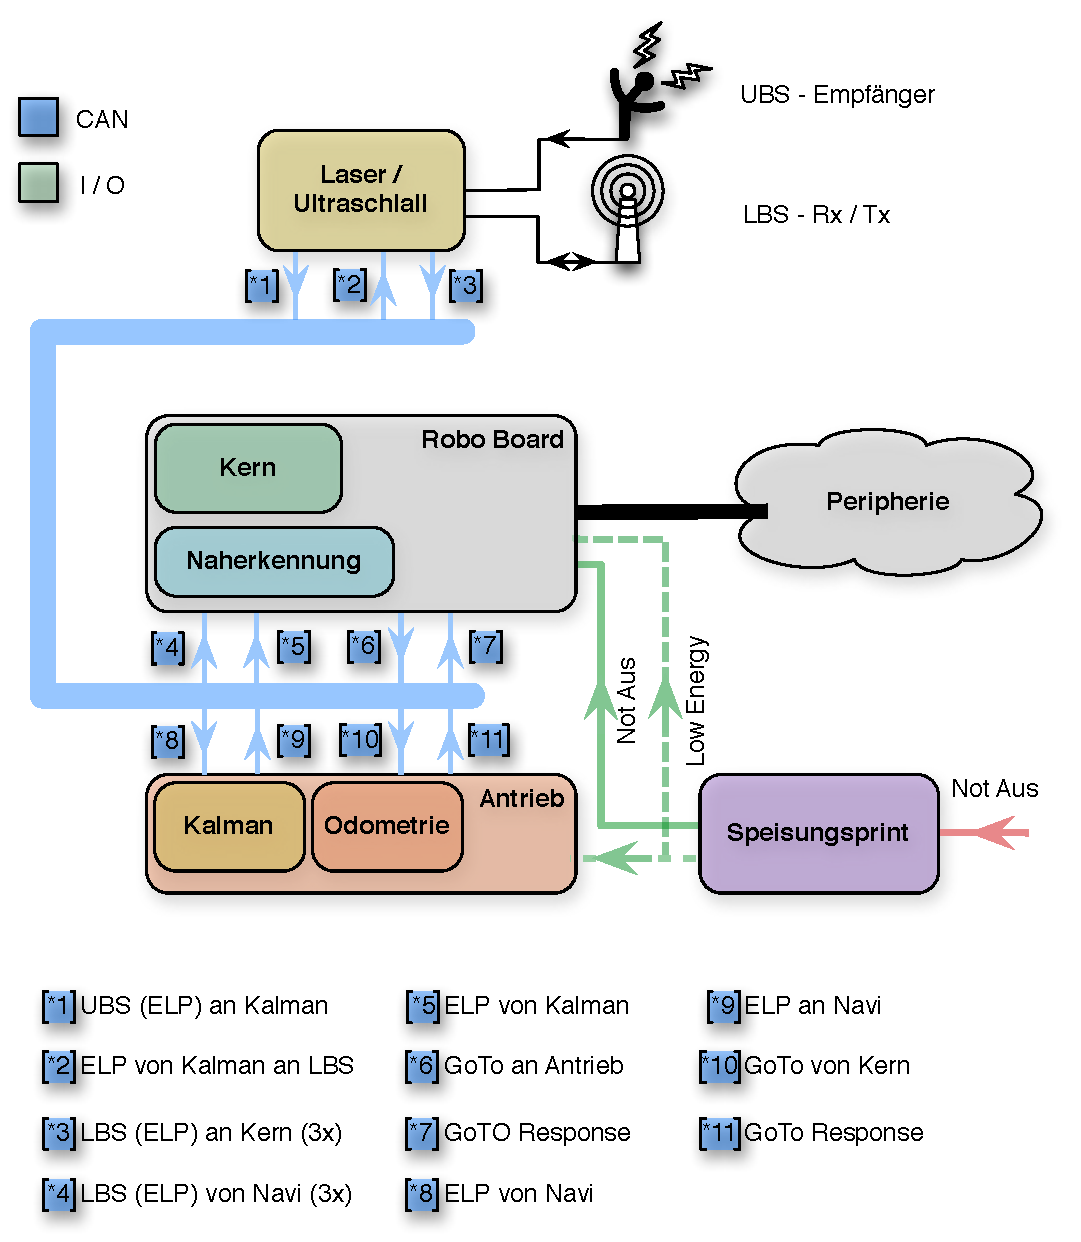
\includegraphics[scale=0.6]{content/image/3_module_im_roboter}
    		\caption{Gliederung kleiner Roboter}
    		\label{abb:gliederung_kleiner_roboter}
    	\end{figure}	
    	
		\begin{description}
			\item[Kernknoten] Der Kernknoten bestehend aus einem RoboBoard ist f�r die gesamte Steuerung des Roboters verantwortlich. Der Kernknoten �bernimmt die strategischen Abl�ufe, so wie die Kommunikation mit den anderen Modulen. Zus�tzlich ist im kleinen Roboter aus Platzgr�nden auch die Naherkennung auf dem Kernknoten umgesetzt.
			%
			\item[Navigation] Damit der Roboter zu jederzeit wissen kann, wo er sich befindet, muss eine Navigationseinheit umgesetzt werden. Diese wird mittels Ultraschall 		und / oder Laser umgesetzt. Wichtig beim Navigationsmodul ist, dass diese auch f�r die Kommunikation zwischen den Robotern verantwortlich sind.
			%
			\item[Antrieb] Der Antrieb ist eines der wichtigsten Module in unserem Roboter. Der antrieb steuert die Motoren an, rechnet Routen aus, um Zielpositionen zu erreichen und liest die Odometrie des Roboters aus. Weiter wird auf der Antriebseinheit das Kalmanfilter implementiert, welches die Positionsbestimmung des Roboters verbessern soll.
			%
			\item[Speisung] Da der Roboter mit 22.2 V Lithium Akkus gespiesen wird, ist es n�tig einen zus�tzlichen Speisungsprint zu verbauen, so dass auch  Spannungen wie 5 V Logik zur Verf�gung stehen. Der Speisungsprint �berwacht weiter die Akkuspannungen und kann im falle eines Not Aus die Stromzufuhr zu den Aktoren des Roboters kappen.
			%
			\item[Peripherie] Damit der Roboter mit der Umwelt interagieren kann, m�ssen verschiedene Sensoren und Aktoren angesteuert werden. Diese beschr�nken sich beim kleinen Roboter auf ein paar Servos, Taster und Sensoren f�r die Naherkennung.\par
		\end{description}
		%
		Damit die verschiedenen Module des Roboters miteinander Kommunizieren k�nnen, werden diese mittels CAN-Schnittstelle miteinander verbunden. Auf die Kommunikation wird im Abschnitt \ref{s:kommunikation} auf Seite \pageref{s:kommunikation} genauer eingegangen.
%
%Kapitel 4: Mechanik
%%%%%%%%%%%%%%%%%%%%%%%%%%%%%%%%%%%%%%%%%%%%%%%%%%%%%%%%%%%%%%%%%%%%%%%%%%%%%%%
% Titel:   Mechanik
% Autor:   rohrp1, roth3
% Datum:   13.12.2013
% Version: 0.0.1
%%%%%%%%%%%%%%%%%%%%%%%%%%%%%%%%%%%%%%%%%%%%%%%%%%%%%%%%%%%%%%%%%%%%%%%%%%%%%%%
%
%:::Change-Log:::
% Versionierung erfolgt auf folgende Gegebenheiten: -1. Release Versionen
%                                                   -2. Neue Kapitel
%                                                   -3. Fehlerkorrekturen
%
% 0.0.1       Erstellung der Datei
%%%%%%%%%%%%%%%%%%%%%%%%%%%%%%%%%%%%%%%%%%%%%%%%%%%%%%%%%%%%%%%%%%%%%%%%%%%%%%%    
\chapter{Mechanik}\label{ch:mechanik}
	%Im folgenden Kapitel wird auf den Teilbereich der Mechanik eingegangen.
	%
	%
	% Konzeptphase
	\section{Konzeptphase}\label{s:konzeptphase}
		Die L�sungsans�tze der Aufgaben Mammut und Fresko werden in einem Morphologischen Kasten festgehalten. Die \acrfull{ac:pa1} beinhaltet prim�r die Aufgaben Mammut und Fresko. Die Funny-Action (Netzaufgabe) wird allerdings nicht ausseracht gelassen, da eventuell Synergien entstehen. Die Aufgabe Netz wird grunds�tzlich in der \gls{ac:pa2} erarbeitet und wird deshalb nicht weiter dokumentiert. 
		%
		%
		\subsection{Morphologischer Kasten}\label{ss:morph_kasten}
			Die Gesamtaufgabe wurde in Teilfunktionen aufgeteilt. Dabei ist die Mammutaufgabe in vier und die Freskoaufgabe in drei Teilfunktionen aufgeteilt (Tabelle \ref{tab:teilfunktionen_mammut} und \ref{tab:teilfunktionen_fresko}). Die Teilfunktionen sind zu diesem Zeitpunkt in sich unabh�ngig und beliebig kombinierbar. F�r die einzelnen Teilfunktionen sind mehrere L�sungsprinzipien erarbeitet.
			%
			%\subsubsection*{Mammut}
				\begin{table}[htbp]
	               \centering
	               \begin{tabularx}{\textwidth}{|l|X|} 
	                   \hline
	                   \rowcolor{bfhblue}
	                   \textcolor{white}{Teilfunktion} & \textcolor{white}{Erl�uterung}\\
	                   \hline
	                   Speicher & Speicherung der Speere (Tischtennisb�lle) innerhalb des Roboter\\
	                   \hline
	                   Vereinzler & Vereinzelung und Zuf�hrung von Speicher zu Wurfmechanismus\\
	                   \hline
	                   F�hrung & Geschossf�hrung nach Abschuss\\
	                   \hline
	                   Wurfmechanismus & Abschussmechanismus mit deren Ausl�sung\\
	                   \hline
	               \end{tabularx}
	               \caption{Teilfunktionen Mammut}
	               \label{tab:teilfunktionen_mammut}  
	           \end{table}
           %
           %\subsubsection*{Fresko}
           		\begin{table}[htbp]
	          		\centering
	          		\begin{tabularx}{\textwidth}{|l|X|} 
		              \hline
		              \rowcolor{bfhblue}
		              \textcolor{white}{Teilfunktion} & \textcolor{white}{Erl�uterung}\\
		              \hline
		              Speicher & Speicherung der Bilder innerhalb des Roboters\\
		              \hline
		              Ankleben & Mechanismus zum Ausfahren, sowie Ausgabe der Bilder aus Speicher\\
		              \hline
		              Positionieren & Positionierung der Bilder am Fresko\\
		              \hline
	          		\end{tabularx}
	          		\caption{Teilfunktionen Fresko}
	          		\label{tab:teilfunktionen_fresko}  
	      		\end{table}	
	      		\newpage
		%
		%
		\subsection{Testreihe}\label{ss:testreihe}
			Um eine gute Absch�tzung und Beurteilung der Wurfmechanismen zu erzielen, sind einfache Prototypen der einzelnen L�sungsprinzipien erarbeitet worden. Diese sind auf ihre Funktionalit�t und Treffsicherheit mit verschiedenen Parametern zu pr�fen. Die Resultate sind ein wichtiger Bestandteil der Nutzwertanalyse (siehe Tabelle \ref{tab:resultate_testreihe} auf Seite \pageref{tab:resultate_testreihe}). Die weiteren Teilfunktionen sind explizit zu testen.
			%
			\subsubsection{Resultate}\label{sss:resultate}
				Im Vorfeld wurden L�sungen �ber einen Hubmagnet und mittels Druckluft in Betracht gezogen. Diese wurde nach ersten Tests sofort wieder verworfen.  Die Testprotokolle sind im Anhang \ref{ch:konzeptphase_mechanik} \textit{Konzeptphase Mechanik} ab Seite \pageref{ch:konzeptphase_mechanik} zu finden.
				%
				\begin{table}[htbp]
                \centering
                \begin{tabularx}{\textwidth}{|l|X|c|} 
                    \hline
                    \rowcolor{bfhblue}
                    \textcolor{white}{L�sungsprinzip} & \textcolor{white}{Resultat} & \textcolor{white}{Versuchsaufbau}\\
                    \hline
                    Reibrad
                    &
                    \tableitemize 
                    \begin{itemize} 
                        \item Grosse Streuung
                        \item Schwingungen
                        \item Velcro wird abgenutzt
                    \end{itemize} 
                    & 
                    \multirow{1}{*}{\imagetotab[width=4cm]{content/image/4_reibrad}}\\
                    &&\\
                    \hline
                    %
                    Impeller
                    &
                    \tableitemize 
                    \begin{itemize} 
                        \item Kleine Streuung
                        \item Vereinzelung n�tig
                        \item Elektrische Leistung
                        \item L�rmentwicklung
                    \end{itemize} 
                    & 
                    \multirow{1}{*}{\imagetotab[width=4cm]{content/image/4_impeller}}\\
                    %
                    \hline
                    %
                    Blattfeder Spickspiel
                    &
                    \tableitemize 
                    \begin{itemize} 
                        \item Kleine Streuung
                        \item Vereinzelung n�tig
                        \item Fehleranf�lligkeit
                    \end{itemize} 
                    & 
                    \multirow{1}{*}{\imagetotab[width=4cm]{content/image/4_blattfeder_spickspiel}}\\
                    &&\\
                    \hline
                    %
                    Hubbalken mit Rohrf�hrung
                    &
                    \tableitemize 
                    \begin{itemize} 
                        \item Klein Speicher n�tig
                        \item Keine Fahrwege
                        \item Grosse Spannkraft
                        \item Schlag
                    \end{itemize} 
                    & 
                    \multirow{1}{*}{\imagetotab[width=4cm]{content/image/4_hubbalken_mit_rohrfuehrung}}\\
                    %&&\\
                    \hline
                    %
                    Hubbalken mit Stabf�hrung
                    &
                    \tableitemize 
                    \begin{itemize} 
                        \item Klein Speicher n�tig
                        \item Keine Fahrwege
                        \item Grosse Spannkraft
                        \item Schlag
                        \item evtl. nicht Regelkonform
                    \end{itemize} 
                    & 
                    \multirow{1}{*}{\imagetotab[width=4cm]{content/image/4_hubbalken_mit_stabfuehrung}}\\
                    %&&\\
                    \hline
                    %
                    Blattfeder
                    &
                    \tableitemize 
                    \begin{itemize} 
                        \item Kleine Streuung
                        \item Keine Vereinzelung
                        \item Kompakt
                        \item Fahrwege n�tig
                    \end{itemize} 
                    & 
                    \multirow{1}{*}{\imagetotab[width=4cm]{content/image/4_blattfeder}}\\
                    %
                    \hline
                \end{tabularx}
                \caption{Resultate Testreihe}
                \label{tab:resultate_testreihe}  
            \end{table}
            \FloatBarrier
     	%
     	%
     	\subsection{Bewertung}\label{ss:bewertung}
     		Die Bewertung der verschiedenen L�sungsprinzipien beider Aufgaben erfolgt durch eine gewichtete Nutzwertanalyse. Um eine m�glichst gute und fundierte Bewertung zu erlangen, definiert das \acrfull{ac:kernteam}, dass mehrere Personen eine Bewertung abgeben.
     		%
     		Eine erste Bewertung erarbeiten die beiden Maschinenbaustudenten des \gls{ac:kernteam} und der Assistent Reto Schmutz. Eine zweite Bewertung erfolgt durch die Elektrostudenten des \gls{ac:kernteam}. Daraus generiert eine Gesamtbewertung seitens \gls{g:eurobot}-Team.
     		%
     		Um Vorurteile sowie Entwicklungsblindheit ausschliessen zu k�nnen, ist eine Bewertung durch die beiden Herren Walter G�ller, Dozent f�r Produktentwicklung und zust�ndiger Betreuer, und Bruno Niklaus Technischer Mitarbeiter HTI erfolgt. Die Bewertungen sind im Plenum diskutiert und verglichen worden. 
     		%
     		Die Bewertung ist mit den in den Tabellen \ref{tab:kriterien_und_gewichtung_mammut} und \ref{tab:kriterien_und_gewichtung_fresko} definierten Kriterien erfolgt.\par 
     		%
     		\begin{table}[htbp]
          		\centering
          		\begin{tabular}{|l|c|} 
					\hline
					\rowcolor{bfhblue}
					\textcolor{white}{Technische Aspekte} & \textcolor{white}{Gewichtung}\\
					\hline
					Treffsicherheit & 3\\
					\hline
					Fehleranf�lligkeit & 2\\
					\hline
					Baugr�sse & 1\\
					\hline
					Zuf�hrung/Speicherung & 2\\
					\hline
					Wurfausl�sung & 2\\
					\hline
					\rowcolor{bfhblue}
					\textcolor{white}{Wirtschaftliche Aspekte} & \textcolor{white}{Gewichtung}\\
					\hline
					Konstruktiver Aufwand & 3\\
					\hline
					Herstellungsaufwand & 2\\
					\hline
					Elektronischer Aufwand & 2\\
					\hline
					Kosten & 1\\
					\hline
					Zeitaufwand (Spiel) & 2\\
					\hline
				\end{tabular}
          		\caption{Kriterien und Gewichtung Mammut}
          		\label{tab:kriterien_und_gewichtung_mammut}  
      		\end{table}	
      		%
      		\begin{table}[htbp]
          		\centering
          		\begin{tabular}{|l|c|} 
					\hline
					\rowcolor{bfhblue}
					\textcolor{white}{Technische Aspekte} & \textcolor{white}{Gewichtung}\\
					\hline
					Zug�nglichkeit Nachladen & 3\\
					\hline
					Fehleranf�lligkeit & 2\\
					\hline
					Baugr�sse & 1\\
					\hline
					Flexibilit�t & 2\\
					\hline
					\rowcolor{bfhblue}
					\textcolor{white}{Wirtschaftliche Aspekte} & \textcolor{white}{Gewichtung}\\
					\hline
					Konstruktiver Aufwand & 3\\
					\hline
					Herstellungsaufwand & 2\\
					\hline
					Elektronischer Aufwand & 2\\
					\hline
					Kosten & 1\\
					\hline
				\end{tabular}
          		\caption{Kriterien und Gewichtung Fresko}
          		\label{tab:kriterien_und_gewichtung_fresko}  
      		\end{table}	
      		%
      		\FloatBarrier
      		Die Nutzwertanalyse sind im Anhang \ref{ch:konzeptphase_mechanik} \textit{Konzeptphase Mechanik} ab Seite \pageref{ch:konzeptphase_mechanik} zu finden.
		%
		%
		\subsection{Entscheid}\label{ss:entscheid}
			\paragraph{Mammut}
			%\subsubsection{Mammut}
				Die Nutzwertanalyse ergibt eine klare F�hrung des Blattfedersystems (Abbildung \ref{abb:abschussmechanismus}). Die Blattfeder zeichnet sich insbesondere durch eine sehr gute Treffsicherheit, die geringe Fehleranf�lligkeit und eine einfache Zuf�hrung ohne Vereinzelung aus (Abbildung \ref{abb:speicherung}). Dieses System wird nun weitergezogen.
				%
				%
				\begin{figure}[htbp] %htbp
					\centering
					\begin{subfigure}[b]{0.49\textwidth}
						\centering
						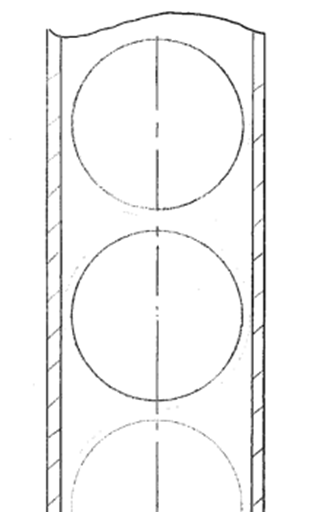
\includegraphics[scale=0.3]{content/image/4_speicher_speer}  
						\caption{Speicherung}
						\label{abb:speicherung}          
					\end{subfigure}
					\begin{subfigure}[b]{0.49\textwidth}
						\centering
						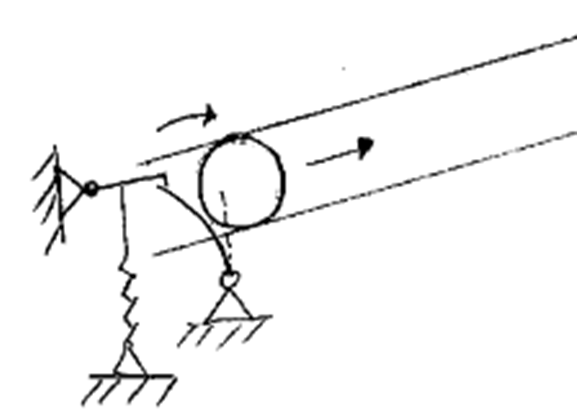
\includegraphics[scale=0.3]{content/image/4_abschussmech_blattfeder}  
						\caption{Abschlussmechanismus Blattfeder} 
						\label{abb:abschussmechanismus}         
					\end{subfigure}
					\caption{Entscheid Mammut}
					\label{abb:entscheid_mammut}
		    	\end{figure}
		   	%
		   	%\newpage
			%\subsubsection{Fresko}
			\paragraph{Fresko}
				Nach der Nutzwertanalyse zeigt sich, dass die Variante mit dem Drehpunkt (Abbildung \ref{abb:abschussmechanismus_fresko}) als beste Variante bewertet wurde. Die Wahl ist vor allem aus der Anzahl einzusetzende Aktoren und auf deren Einfachheit der Konstruktion zur�ckzuf�hren. Diese Variante wird somit weitergezogen und erarbeitet.  	
      		 	%
				\begin{figure}[htbp] %htbp
					\centering
					\begin{subfigure}[b]{0.49\textwidth}
						\centering
						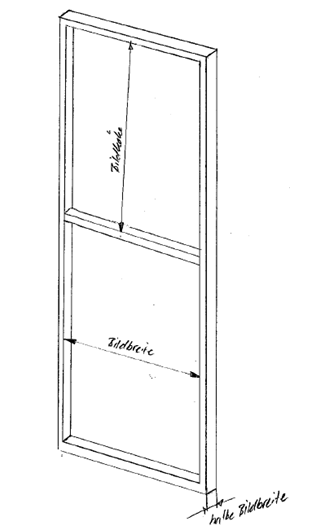
\includegraphics[scale=0.3]{content/image/4_bilderspeicher}  
						\caption{Speicherung}
						\label{abb:speicherung_fresko}          
					\end{subfigure}
					\begin{subfigure}[b]{0.49\textwidth}
						\centering
						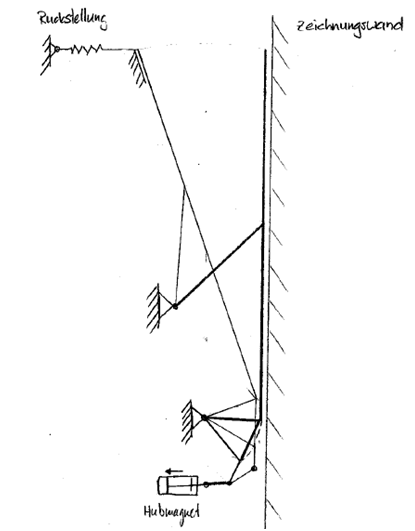
\includegraphics[scale=0.3]{content/image/4_bildermontagemech}  
						\caption{Abschlussmechanismus mit Drehpunkt} 
						\label{abb:abschussmechanismus_fresko}         
					\end{subfigure}
					\caption{Entscheid Mammut}
					\label{abb:entscheid_fresko}
		    	\end{figure}
		    	%\FloatBarrier
	%
	%
	% Ausarbeitungsphase
	\section{Ausarbeitungsphase}\label{s:ausarbeitungsphase}
		Die Mechanismen f�r die Fresko- und die Mammutaufgabe m�ssen beide im kleinen Roboter Platz finden. Aus diesem Grund ist die Baugr�sse der Systeme von grosser Bedeutung. Alle Bauteile sind im \textsf{Unigraphic NX8.0} modelliert. Die dazugeh�rigen Fertigungszeichnungen sind im Anhang \ref{ch:zeichnungen_cad} \textit{Zeichnungen CAD} ab Seite \pageref{ch:zeichnungen_cad} einzusehen.
		%
		%
		\subsection{Fresko}\label{ss:fresko}
			%
			%\subsubsection{Allgemeine Beschreibung}	
				Die Bilder werden vertikal und �bereinander in einen Bilderrahmen eingelegt. Der Rahmen wird �ber ein digitales Servo der Firma Hitec linear ausgefahren. Die Bewegung l�uft auf zwei kleinen F�hrungsschienen der Firma Igus. Aus Platzgr�nden wird das gesamte Modul auf den Kopf gedreht und an der zweiten Zweischenplatte aufgeh�ngt.(Abbildung \ref{abb:linearmodul})
				%
				\image{content/image/4_linearmodul}{scale=.3}{htbp}[Linearmodul][abb:linearmodul]
			%
			\subsubsection{Eingekaufte Komponente}
				\begin{description}
					\item[Servo] Hitec, digitales Standard Servo HS 5645 (siehe Anhang D \textit{Datenbl�tter})
					\item[F�hrungen] Igus GmbH, N-Flachf�hrung [17] (siehe Anhang D \textit{Datenbl�tter})
					\item[Lagerbuchsen] Igus GmbH, iglidur J Gleitlager, Form F (siehe Anhang D \textit{Datenbl�tter})
					\item[Tastsensoren] Omron, Snap Action Switch D2F-01L (siehe Anhang D \textit{Datenbl�tter})
				\end{description}
			%
			\subsubsection{Servo}
				Die Baugr�sse des Sevos ist im vorgesehenen Bereich des Roboters nicht von grosser Bedeutung. Deshalb haben wir uns hier f�r ein digitales Standard Servo entschieden. Das digitale Servo bringt zu dem gegen�ber einem analogen den Vorteil einer einfacheren Kalibrierung.
			%
			\subsubsection{F�hrungen und Lagerbuchsen}
				Auf das System wirken zu keinem Zeitpunkt grosse Kr�fte. Aus diesem Grund setzen wir f�r die Linearf�hrung kleine N-F�hrungen der Firma Igus ein. Die F�hrung zeichnet sich insbesondere durch das niedrige Gewicht und die geringen Reibwerte ohne zus�tzliche Schmierung aus.\par 
				%
				Auch die Lagerbuchsen dienen lediglich zur Verminderung der Reibwerte.
			%
			\subsubsection{Tastsensoren}
				Die Sensoren der Firma Omron zeichnen sich insbesondere durch die sehr geringe Baugr�sse aus. Sie werden pro Sensor �ber zwei Langl�cher Verschraubt. Das erm�glicht uns ein flexibles einstellen der Position.		
			%
			\subsubsection{M�gliche Fehler}
				Damit gr�ssere Nacharbeitungen vermieden werden k�nnen, wird bereits in der Ausarbeitungsphase versucht alle m�glichen Fehler aufzudecken und eine L�sung f�r die Probleme zu konstruieren. Die wichtigsten Fehlerquellen und die Massnahmen um diese zu verhindern, sind aus Tabelle \ref{tab:fehler_fresko} zu entnehmen.	
				%
				\begin{table}[t]
	          		\centering
	          		\begin{tabularx}{\textwidth}{|p{6cm}|X|} 
					    \hline
					    \rowcolor{bfhblue}
					    \textcolor{white}{M�gliche Fehler} & \textcolor{white}{Massnahmen}\\
					    \hline
					    Herausfallen der Bilder aus Rahmen & Damit die Bilder durch Vibrationen gegen das Rausfallen gesichert sind, sind sie mittels zwei Schaumstoffb�ndern und jeweils zwei Gewindestifte, welche die Klemmkraft im Rahmen einstellbar machen, gesichert (Abbildung \ref{abb:abschussmechanismus}).\\
					    \hline
					    Kollision der gegnerischen Bilder auf der Klettwand. (Bilder kleben nicht und bleiben im Rahmen) & Die Bilder werden �ber einen mechanischen Tastsensor �berwacht. Bleibt das Bild nach Anpressen an das Fresko nicht haften und somit immer noch im Rahmen, bleibt der Kontakt �ber den Tastsensor bestehen. Der Roboter f�hrt dann eine neue Position an und wiederholt die Montage der Bilder (Abbildung \ref{abb:bildueberwachung}).\\
					    \hline
					    Nicht Ber�hren der Klettwand & Ein mechanischer Tastsensor der sich im Zentrum des Bilderrahmens befindet, gibt an, sobald die Bilder die Wand ber�hren. Somit muss der Roboter gegen die Wand fahren bis der Tastsensor get�tigt wird (Abbildung \ref{abb:absturzsicherung}).\\
					    \hline
					    Schr�ges Anfahren der Klettwand & Der Bilderrahmen wird zentrisch verdrehbar gelagert. Damit kann ein Winkelfehler von beidseitig 10� aufgenommen werden (Abbildung \ref{abb:linearmodul}).\\
					    \hline
	          		\end{tabularx}
	          		\caption{Teilfunktionen Fresko}
	          		\label{tab:fehler_fresko}  
	      		\end{table}	
	      		%
	      		\FloatBarrier
				\begin{figure}[htbp] %htbp
					\centering
					\begin{subfigure}[b]{0.49\textwidth}
						\centering
						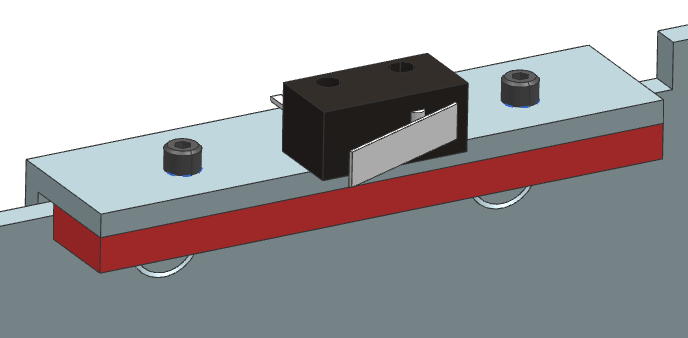
\includegraphics[height=2.5cm]{content/image/4_tastsensoren_absturzsicherung}  
						\caption{Absturzsicherung}
						\label{abb:absturzsicherung}          
					\end{subfigure}
					\begin{subfigure}[b]{0.49\textwidth}
						\centering
						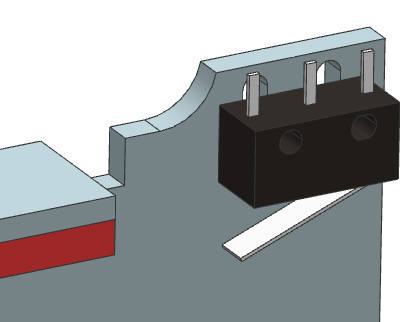
\includegraphics[height=2.5cm]{content/image/4_tastsensoren_bildueberwachung}  
						\caption{Bild�berwachung} 
						\label{abb:bildueberwachung}         
					\end{subfigure}
					\caption{Tastsensoren}
					\label{abb:tastsensoren}
		    	\end{figure}
		    	%
		    %
		    \newpage
		    \subsubsection{Bilder}
		    	Die Abmasse der Bilder ist im Reglement mit minimalen und maximalen Massen genau definiert \cite[]{lit:eurobot}. Der Entscheid f�llt sofort auf die kleinstm�gliche Abmessung. Dies erm�glicht eine minimale Baugr�sse und minimiert das Risiko einer Kollision mit gegnerischen Bildern auf der Klettwand. Um ein optimales Kleben der Bilder zu erreichen, sind die Klettstreifen auf den Bildern vertikal angeordnet. Damit kann garantiert werden, dass jedes Bild mindestens auf zwei der horizontal angeordneten Steifen der Wand haftet.\par 
		    	%
		    	Weiter m�ssen die Bilder in den jeweiligen Team-Farben eingef�rbt werden.\par  
		    	%
		    	Damit die Bilder an der Wand haften bleiben, d�rfen sie nicht zu schwer sein. Die Bilder werden deshalb aus Polyacetal (POM) angefertigt, dies ergibt ein Gewicht von rund 85 Gramm pro Bild. Zudem ist POM einfach zu bearbeiten.
		%
		%
		\newpage
		\subsection{Mammut}
			%
			%\subsubsection{Allgemeiner Beschrieb}
				Die Speere sind zu je 3 St�ck in den zwei Magazinrohren (Abbildung \ref{abb::abschussvorrichtung_mammut_komplett}) vorg�ngig gespeichert. Dazu sind die Magazine an der oberen Decke des Roboters offen, so dass die Speere einfach in die Magazinrohre zu geben sind. Der unterste Speer ist bereits in Abschussposition. Pro Abschuss werden zwei Speere abgeschossen, somit sind pro Spiel drei H�be zu t�tigen.\par
				\image{content/image/4_abschussmech_komp}{scale=.35}{htbp}[Abschussvorrichtung Mammut komplett][abb::abschussvorrichtung_mammut_komplett] 
				%
				Die Beschleunigungsenergie erfahren die Speere �ber eine Blattfeder. Eine Blattfeder pro Abschussrampe (Abbildung \ref{abb:abschussvorrichtung_mammut}). Diese wird durch eine Klinke gegriffen und gespannt. Die Ausl�sung der Blattfeder wird durch die Durchbiegung (Abbildung \ref{abb:abschussvorrichtung_mammut}) der Feder erlangt. Durch die Biegung verliert die Klinke den Eingriff auf die Blattfeder. %\par 
				%
				Die Klinke ist in die Klinkenwelle integriert . Die beiden Klinkenwellen sind miteinander verbunden und werden durch ein Servo angesteuert. (Abbildung \ref{abb:abschussvorrichtung_mammut}) %\par 
				%
				Nach dem Abschuss der zwei Speere auf der Abschussrampe fallen die n�chsten zwei in die Abschussposition.
				%
				\image{content/image/4_zeichnung-2}{scale=.3}{htbp}[Abschussvorrichtung Mammut][abb:abschussvorrichtung_mammut]
			%
			\subsubsection{Eingekaufte Komponente}
				\begin{description}
					\item[Servo] Hitec, Servo HS-5125 MG (siehe Anhang D \textit{Datenbl�tter})
					\item[Gleitlager] Igus GmbH, iglidur J Gleitlager (siehe Anhang D \textit{Datenbl�tter})
				\end{description}
			%
			\subsubsection{Servo}
				Die Baugr�sse ist in diesem Bereich Massgebend, zudem sind die Befestigungsanschl�sse relevant. Deshalb kommt in dieser Anwendung ein flaches digitales Servo zum Einsatz. 
			%
			\subsubsection{Gleitlager}
				Das Gleitlager wird nur in axialer Richtung belastet. Dabei sind keine grossen Belastungen aufzunehmen. Die Standartgleitbuchse kann mit ihren Reibwerten diese Anforderungen erf�llen.
			%
			\subsubsection{Einstellm�glichkeiten}
				\paragraph{Abschusswinkel}
					Der Abschusswinkel kann zwischen 15� und 25� zur Horizontalen eingestellt werde(Abbildung \ref{abb:abschussvorrichtung_15} und \ref{abb:abschussvorrichtung_25}). Der Abschusswinkel ist nicht variabel von Abschuss zu Abschuss und er gilt f�r beide Abschussrampen. 
					%
					\begin{figure}[htbp] %htbp
						\centering
						\begin{subfigure}[b]{0.49\textwidth}
							\centering
							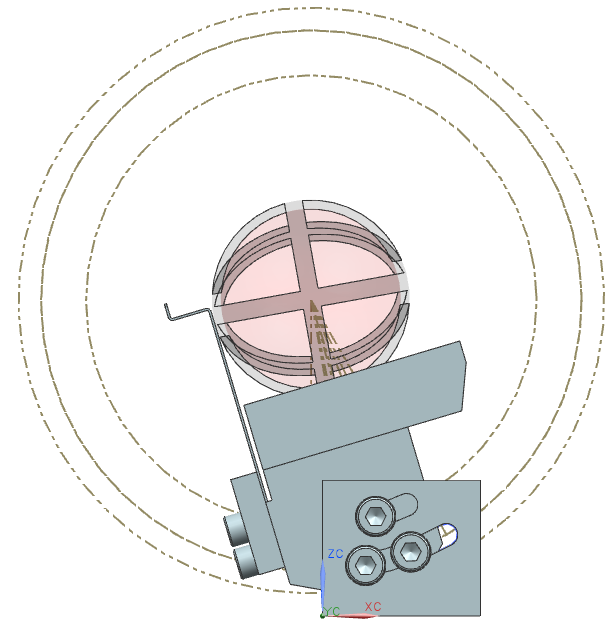
\includegraphics[height=4.5cm]{content/image/4_abschussmech_15grad}  
							\caption{Abschussvorrichtung mit 15� Abschusswinkel}
							\label{abb:abschussvorrichtung_15}          
						\end{subfigure}
						\begin{subfigure}[b]{0.49\textwidth}
							\centering
							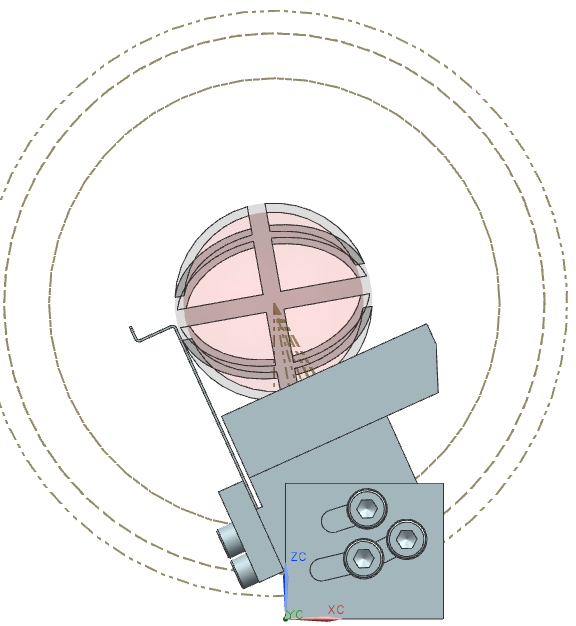
\includegraphics[height=4.5cm]{content/image/4_abschussmech_25grad}  
							\caption{Abschussvorrichtung mit 25� Abschusswinkel} 
							\label{abb:abschussvorrichtung_25}         
						\end{subfigure}
						\caption{Einstellm�glichkeiten Abschussvorrichtung}
						\label{abb:einstellmoeglichkeiten_abschlussvorrichtung}
			    	\end{figure}
					%
					Damit die Abschussposition der Speere nicht durch den Abschusswinkel abh�ngig ist, wurde das Zentrum der Winkeleinstellung in das Zentrum des Speers an Abschussposition gew�hlt. (Abbildung \ref{abb:abschussvorrichtung_15} und \ref{abb:abschussvorrichtung_25})
				\paragraph{Vorspannung Blattfeder}
					Wie bereits erw�hnt verliert die Klinke den Eingriff an der Blattfeder durch die Verbiegung der Blattfeder.  die Verformung der Feder durch Angriff der Kraft an der Eingriffstelle der Klinke ist mit Ansys Workbench simuliert worden. (Abbildung \ref{abb:verfomung_blattfeder})
					%
					\begin{figure}[htbp] %htbp
						\centering
						\begin{subfigure}[b]{0.49\textwidth}
							\centering
							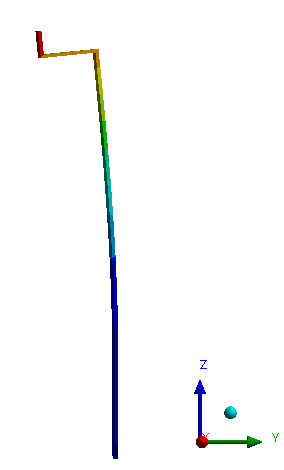
\includegraphics[height=5.5cm]{content/image/4_verformung_blattfeder_ANSYS}  
							\caption{Verformung der Blattfeder}
							\label{abb:verfomung_blattfeder}          
						\end{subfigure}
						\begin{subfigure}[b]{0.49\textwidth}
							\centering
							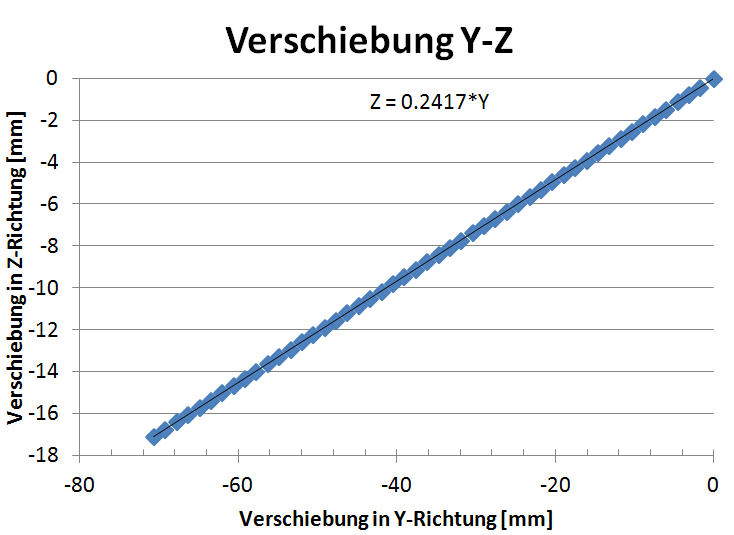
\includegraphics[height=5.5cm]{content/image/4_verformung_blattfeder}  
							\caption{Verformung des Eingriffsbereichs der Kinke in X und Z Richtung} 
							\label{abb:verformung_klinke}         
						\end{subfigure}
						\caption{Einstellm�glichkeiten Abschussvorrichtung}
						\label{abb:einstellmoeglichkeiten_blattfeder}
			    	\end{figure}	
					%
					Die Verformung ist linear und betr�gt rund 13.5� zur horizontalen. (Abbildung \ref{abb:verformung_klinke})\par 
					%
					\newpage
					Der Federspannweg wird durch die �nderung des Winkels der Klinkenwellenachse zur Verformungsgeraden realisiert. Die Einstellungen sind vorg�ngig zu t�tigen. (Abbildung \ref{abb:ausgangsposition_0}-\ref{abb:abschussposition_13})
					\begin{figure}[htbp] %htbp
						\centering
						\begin{subfigure}[b]{0.49\textwidth}
							\centering
							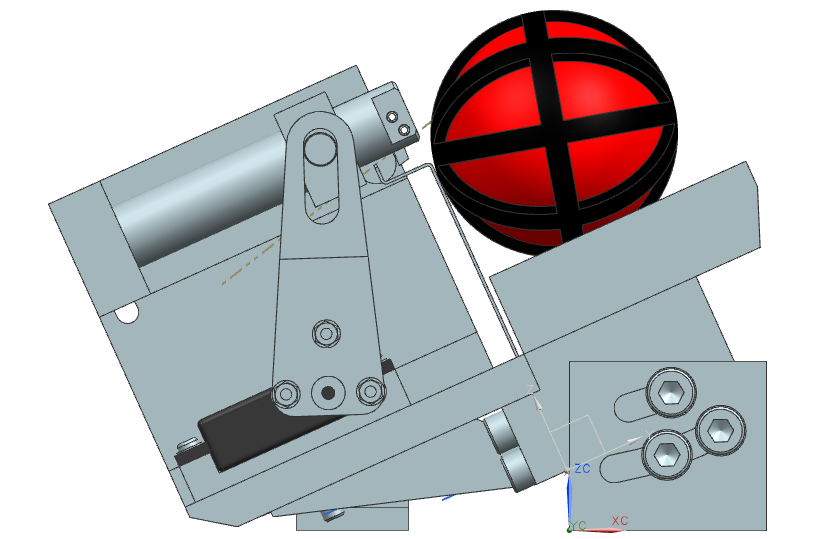
\includegraphics[height=4.5cm]{content/image/4_abschussmech_federspanner_0grad_vorne}  
							\caption{Ausgangsposition Federspannwinkel 0�}
							\label{abb:ausgangsposition_0}          
						\end{subfigure}
						\begin{subfigure}[b]{0.49\textwidth}
							\centering
							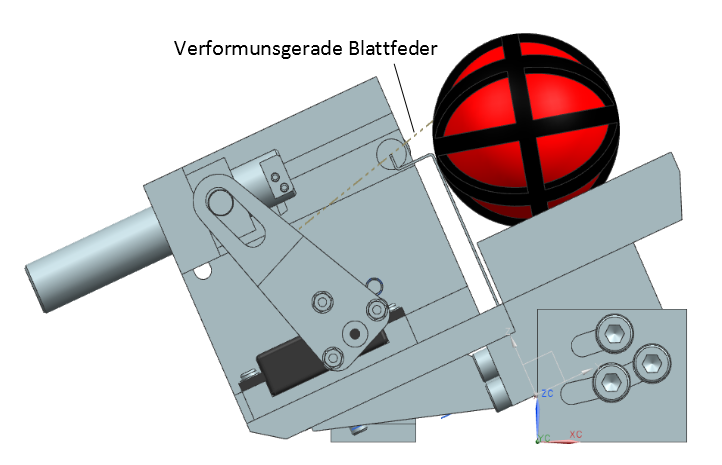
\includegraphics[height=4.5cm]{content/image/4_abschussmech_federspanner_0grad_hinten}  
							\caption{Ausl�seposition Federspannwinkel 0�} 
							\label{abb:ausloeseposition_0}         
						\end{subfigure}
						\begin{subfigure}[b]{0.49\textwidth}
							\centering
							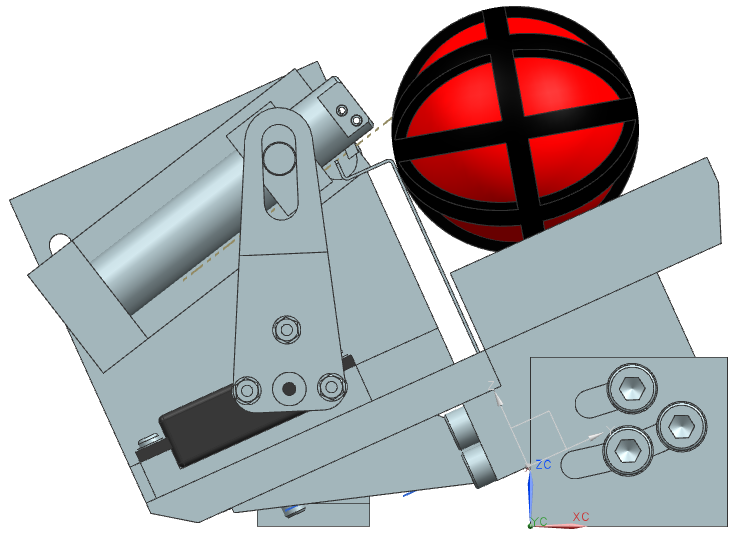
\includegraphics[height=4.5cm]{content/image/4_abschussmech_federspanner_13grad_vorne}  
							\caption{Ausgangsposition Federspannwinkel 13�}
							\label{abb:ausgangsposition_13}          
						\end{subfigure}
						\begin{subfigure}[b]{0.49\textwidth}
							\centering
							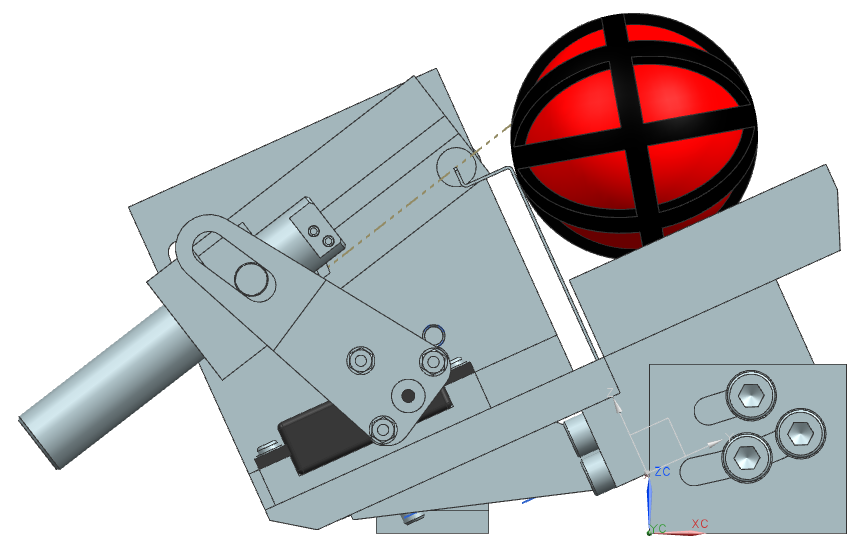
\includegraphics[height=4.5cm]{content/image/4_abschussmech_federspanner_13grad_hinten}  
							\caption{Abschussposition Federspannwinkel 13�} 
							\label{abb:abschussposition_13}         
						\end{subfigure}
						\caption{Einstellm�glichkeiten Federspannwinkel}
						\label{abb:einstellmoeglichkeiten_federspannwinkel}
			    	\end{figure}	
				
%
%Kapitel 5: Software
%%%%%%%%%%%%%%%%%%%%%%%%%%%%%%%%%%%%%%%%%%%%%%%%%%%%%%%%%%%%%%%%%%%%%%%%%%%%%%%
% Titel:   Software
% Autor:   gross10, mert1
% Datum:   22.09.2013
% Version: 0.0.1
%%%%%%%%%%%%%%%%%%%%%%%%%%%%%%%%%%%%%%%%%%%%%%%%%%%%%%%%%%%%%%%%%%%%%%%%%%%%%%%
%
%:::Change-Log:::
% Versionierung erfolgt auf folgende Gegebenheiten: -1. Release Versionen
%                                                   -2. Neue Kapitel
%                                                   -3. Fehlerkorrekturen
%
% 0.0.1       Erstellung der Datei
%%%%%%%%%%%%%%%%%%%%%%%%%%%%%%%%%%%%%%%%%%%%%%%%%%%%%%%%%%%%%%%%%%%%%%%%%%%%%%%    
\chapter{Software}\label{ch:software}\mpar{Dieser Abschnitt entspricht nicht vollst�ndig dem Stand der \gls{ac:pa2}}
	Die Software wird auf einem \textsf{STM32F4 Discovery} von \textsf{STMicroelectronics} implementiert, welches auf einem \gls{g:roboboard} aufgesteckt wird. Das \gls{g:roboboard} ist eine Arbeit des Eurobotteams vom Vorjahr, mit welchem diverse Peripherie angesteuert werden kann.
	%
	%
	%Gliederung
	\section{Gliederung}\label{s:gliederung}
	Die Software wird, wie in Abbildung \ref{abb:structed_design} strukturell dargestellt, in vier Kategorien unterteilt.	
		\image{content/image/5_Structed_Design}{scale=0.5}{htbp}[Structed Design][abb:structed_design]
		%
		\begin{description}
			\item[Applikation] In der Kategorie Applikation werden alle Softwaremodule abgelegt, die zur Steuerung des Roboters ben�tigt werden. Dieser Code greift auf die von den anderen drei Kategorien bereitgestellten Funktonen zu. 
			%
			\item[Lib] In dieser Library werden die Firmware-Funktionen f�r das \gls{g:roboboard} zusammengefasst. Weiter sind auch Funktionen f�r die Kommunikation mit dem Debugger von Atollic\footnote{Atollic TrueSTUDIO ist das von uns ben�tigte Programm f�r die Softwareprogrammierung.} vorhanden, um das Testen von Software zu erleichtern. Mehr dazu im Kapitel \ref{ss:swd} \textit{SWD} ab Seite \pageref{ss:swd}.
			%   
			\item[FreeRTOS] Das Framework \gls{g:rtos} bietet alle Funktionalit�ten, um ein Real Time Operating System auf dem Mikrocontroller realisieren zu k�nnen. Mit Hilfe dessen ist es m�glich quasi parallele Prozesse schreiben zu k�nnen.
			%
			\item[BSP] Im \gls{ac:bsp} ist jener Code zu finden, um die Low Level Funktionen des Mikrocontrollers nutzen zu k�nnen.
		\end{description}
	%
  	%
  	%Applikation
  	\section{Applikation}\label{s:applikation}
  	Alle in der Applikation geschriebenen Module sind als Tasks umgesetzt. Sie dienen vorwiegend der Steuerung und Kommunikation des Roboters. Das Main-Modul startet nach Programmstart alle ben�tigten Tasks und �bergibt die Kontrolle dem Betriebssystem.
  		%Uebersicht
  		\subsection{�bersicht}\label{ss:uebersicht}
  		In Abbildung \ref{abb:task_diagramm} auf Seite \pageref{abb:task_diagramm} ist das Task-Diagramm der Applikationskategorie abgebildet. Dem Diagramm ist das grobe Zusammenspiel der einzelnen Tasks grafisch dargestellt. Es wurden insgesamt f�nf Tasks implementiert. 
  		%
  		\image{content/image/5_Taskdiagramm}{scale=0.75}{htbp}[Task-Diagramm][abb:task_diagramm]
  		%
  		\begin{description}
			\item[Strategy] Der Strategy-Task ist f�r den Ablauf, so wie die Spielmanipulationen zust�ndig.
			%
			\item[Timer] Im Timer-Task wird die Zeitmessung f�r ein Spiel realisiert.
			%
			\item[ELP] Der \acrfull{ac:elp}-Task ruft regelm�ssig die Positionsinformationen der anderen knoten im Roboter ab.
			%
			\item[Rangefinder] Die Naherkennung, welche nicht vom Kernteam umgesetzt wurde, wird in der \gls{ac:pa2} in den Rangefinder-Task implementiert.
			%
			\item[CANGatekeeper] Mit diesem Task kann zwischen den Knoten Kommuniziert werden.
		\end{description}
  		%
  		%Strategie
  		\subsection{Strategy}\label{ss:strategie}
  		Der \texttt{Strategy}-Task ist f�r die Strategie und den Ablauf eines Spiels zust�ndig. In diesem Task werden vordefinierte Spielabl�ufe und Strategien implementiert, welche vor oder auch w�hrend des Spiels abgerufen werden k�nnen. Dies ist notwendig, da der Spielablauf auf Grund der Gegnerroboter nicht  immer gleich ist.
  		%
  		\subsubsection{Design}\label{sss:strategie_design}
  		\image{content/image/5_CRC_Strategy}{scale=0.75}{htbp}[CRC \texttt{Strategy}-Task][abb:crc_strategy]
  		Da der Roboter zum momentanen Zeitpunkt noch nicht besteht, wurde im \texttt{Strategy}-Task noch nicht Alles implementiert. Es werden lediglich einzelne Abl�ufe und Unit Test vorgenommen.
  		%
 		%Zeitmanagement
  		\subsection{Timer}\label{ss:zeitmanagement}
  		Der \texttt{Timer}-Task ist f�r die Spielzeit zust�ndig. Der Task hat als Aufgabe das Messen der bereits vergangenen Spielzeit. Der \texttt{Timer} stellt eine Funktion zur Verf�gung, mit welcher die Zeitmessung gestartet werden kann. Nach Ablauf der 90 Sekunden l�st der \texttt{Timer} eine Flag aus und sendet den Stoppbefehl an den Antrieb.
  		%
  		\subsubsection{Design}\label{sss:timer_design}
  		\image{content/image/5_CRC_Timer}{scale=0.75}{htbp}[CRC Timer-Task][abb:crc_timer]
  		Der Timer-Task besteht zum momentanen Zeitpunkt aus einem Task f�r die Zeitmessung welcher jede Sekunde Ausgerufen wird und zwei Funktionen:
  		\begin{description}
  			\item[\texttt{startTimer()}] Diese Funktion Startet den 90 sec Timer
  			\item[\texttt{getRemainingTime()}] Liefert die Verbleibende Spielzeit in Sekunden zur�ck
  		\end{description}
  		%
  		Der \texttt{Timer} ben�tig den \texttt{CANGatekeeper}, um die Stoppnachricht an die anderen Module zu senden. Dies ist wichtig, da sich der Roboter nach Ablauf der 90 sec nicht mehr bewegen darf.\par
  		%
  		Um die Zeit genau messen zu k�nnen, muss der \texttt{Timer}-Task die h�chste Priorit�t von allen Tasks besitzt. Nur so ist gew�hrleistet, dass die Zeit m�glichst genau gemessen werden kann, da die Verz�gerung zwischen Delay-Ablauf und Taskaufruf m�glichst klein ist. G�be es einen anderen Task mit h�herer Priorit�t, so w�rde der \texttt{Timer} erst nach diesem an die Reihe kommen und so eine falsche Zeitmessung bewirken.
  		%
  		\subsubsection{Defines}\label{sss:timer_defines}
  		Im \texttt{Timer.h} File sind folgende Timerspezifische Defines vorhanden:
  		%
		\begin{description}
	  		\item[\texttt{TIMER\_STOP\_TIME}] Mit diesem Define kann die zu stoppende Zeit eingestellt werden.
	  	\end{description}
  		%
  		%Datenkommunikation
  		\subsection{ELP}\label{ss:datenkommunikation}
  		Der \texttt{ELP}-Task ist f�r die Abfrage der ELP's der anderen Knoten im Roboter zust�ndig. Da Die \gls{ac:can}-Kommunikation als Master Slave implementiert wurde\footnote{siehe Abschnitt \ref{ss:variantenentscheid_ms_mm} \textit{Variantenentscheid Master-Slave Multi-Master} auf Seite \pageref{ss:variantenentscheid_ms_mm}}, muss der Kernknoten alle anderen Informationen der �brigen Knoten regelm�ssig abfragen, so dass die Slaves mith�ren k�nne, um an die entsprechenden Infos zu gelangen.
  		%
  		\subsubsection{Design}\label{sss:datenkommunikation_design}
  		\image{content/image/5_CRC_ELP}{scale=0.75}{htbp}[CRC ELP-Task][abb:crc_elp]
  		Um die ELP's der anderen Knoten im Roboter abfragen zu k�nnen, muss der \texttt{CANGatekeeper} in den \texttt{ELP}-Task eingebunden werden. Es werden insgesamt sechs ELP's angefragt:
  		%
  		\begin{itemize}
	  		\item Laser ELP
	  		\item Ultraschall ELP
	  		\item Kalman ELP
	  		\item Gegner Roboter 1 ELP
	  		\item Gegner Roboter 2 ELP
	  		\item Befreundeter Roboter ELP
  		\end{itemize}
  		%
  		\subsubsection{Defines}\label{sss:datenkommunikation_defines}
  		Da die ELP's der verschiedenen Knoten nicht alle gleich h�ufig abgefragt werden k�nnen oder m�ssen, kann in der \texttt{ELP.h} Datei mittels Defines eingestellt werden, wir oft das jeweilige ELP abgefragt werden soll. Es sind folgende Defines Implementiert worden:
  		%
  		\begin{description}
	  		\item [\texttt{ELP\_LASER\_POSITION\_REQUEST\_RATE}]
	  		\item [\texttt{ELP\_ULTRASONIC\_POSITION\_REQUEST\_RATE}]
	  		\item [\texttt{ELP\_KALMAN\_POSITION\_REQUEST\_RATE}]
	  		\item [\texttt{ELP\_ENEMY1\_POSITION\_REQUEST\_RATE}]
	  		\item [\texttt{ELP\_ENEMY2\_POSITION\_REQUEST\_RATE}]
	  		\item [\texttt{ELP\_CONFEDERATE\_POSITION\_REQUEST\_RATE}]
  		\end{description}
  		%
  		Mit diesen Defines kann nun eingestellt werden, beim wievielten Durchlaufen des \texttt{ELP}-Tasks welches ELP abgefragt werden soll. Weiter kann durch ein Define das Delay des \texttt{ELP}-Tasks eingestellt werden und somit die Geschwindigkeit der mit der der Task wieder aufgerufen wird.
  		%
  		\begin{description}
	  		\item [\texttt{ELP\_TASK\_SPEED}] Updaterate in Millisekunden
  		\end{description}
  		\newpage
  		%
  		%Naherkennung
  		\subsection{Rangefinder}\label{ss:naherkennung}
  		Der \texttt{Rangefinder}-Task �bernimmt die Aufgabe der Naherkennung. Die genaue Dokumentation hierzu ist dem Entsprechenden Teilprojekt von Nicolas K�ser zu entnehmen.
  		%
  		\subsubsection{Design}\label{sss:naherkennung_design}
  		\image{content/image/5_CRC_Rangefinder}{scale=0.75}{htbp}[CRC \texttt{Rangefinder}-Task][abb:crc_rangefinder]
  		Um mit den Sensoren zu interagieren, m�ssen die Firmwaredateien \texttt{i2c.h} und \texttt{gpio.h} importiert werden. 
  		%
  		%Feldbus
  		\subsection{CANGatekeeper}\label{ss:cangatekeeper}\mpar{F�r Informationen zum aktuellen Stand der \gls{ac:pa2} sei auf den Anhang H verwiesen}
  			In Applikationen in denen mehrere neben l�ufigen Threads Tasks vorkommen, kann das Zugreifen auf gemeinsame Ressourcen problematisch sein. Die als Critical Section bezeichneten Codesegmente m�ssen deshalb von Mehrfachzugriffen, respektive Ausf�hrungen gesch�tzt werden. Dazu stehen drei g�ngige M�glichkeiten zur Verf�gung:
  			%
  			\begin{description}
  				\item[Semaphore] Eine Semaphore kann als Schl�sselbund der Informatik verstanden werden. Sie wird vom Betriebssystem zur Verf�gung gestellt. Will eine Parallelit�tseinheit auf eine Critical Section zugreifen, so muss sie zu erst eine Semaphore anfordern. Nach dem Zugriff wird die Semaphore freigegeben und die Ressource ist wieder verf�gbar. Eine Critical Section kann mehrere Semaphoren haben \cite[S.65]{lit:es}.
  				\item[\acrshort{ac:mutex}] Eine \gls{ac:mutex} kann als Semaphore  der L�nge '1' verstanden werden \cite{lit:mutex_vs_semaphore}.
  				\item[Gatekeeper] Ein Gatekeeper ist kein vom Betriebssystem bereitgestelltes Konstrukt\footnote{Dies bezieht sich auf das eingesetzte \gls{g:rtos}}, sondern stellt ein Software Designpattern dar. Dazu wird ein Thread Task erzeugt, der eine Critical Section verwaltet. Ein Datentransfer erfolgt via eines Queues zum Gatekeeper.
  			\end{description}
  			%
  			Die \gls{ac:can}-Schnittstelle stellt eine solche Critical Section dar, weshalb eine der vorangehenden Varianten angewandt werden muss. Da aufbauend auf dem \gls{ac:can}-Protokoll mehrere Kommunikation-Protokolle eingesetzt werden\footnote{siehe dazu Abschnitt \ref{s:kommunikation} ab Seite \pageref{s:kommunikation}} und es keinen Sinn ergibt wenn jede Parallelit�tseinheit diese beinhaltet, scheiden die beiden erst genannten Methoden (\textsf{Semaphore} und \gls{ac:mutex}) aus. Mithilfe eines \texttt{Gatekeepers} k�nnen protokollspezifische Anpassungen an einem zentralen Ort verwaltet werden.\par 
  			%
  			Der \texttt{CANGatekeeper} �bernimmt die folgenden Aufgaben:
  			\begin{itemize}
  				\item Initialisierung des \gls{ac:can}-Interfaces
  				\item Stellt einfache anzuwenden Sendefunktionen zur Verf�gung
  				\item Konvertiert Daten in die entsprechende Kommunikationsprotokolle um\footnote{\acrfull{ac:goto} und \acrfull{ac:elp}}
  				\item Das Verteilen empfangener Daten an eingetragene Empf�nger
  			\end{itemize}
  			%
  			F�r die Funktion werden die Module \texttt{app\_config}, \texttt{can} (siehe Abschnitt \ref{ss:Control_area_network} \textit{Control Area Network} auf Seite \pageref{ss:Control_area_network}), \texttt{queue} (\textsf{FreeRTOS}) und \texttt{stm32f4xx\_can} (\textsf{BSP}) vorausgesetzt. Der \texttt{CANGatekeeper} wird der Sektion der \textsf{HW-Tasks} zugeordnet, sprich er enth�lt Abh�ngigkeiten zu Bereichen \textsf{FreeRTOS}, \textsf{Firmware} und \textsf{\gls{ac:bsp}}. Eine �bersicht �ber das Modul \texttt{CANGatekeeper} bietet die Abbildung \ref{abb:crc_cangatekeeper}.
  			\image{content/image/5_CRC_CANGatekeeper}{scale=0.75}{htbp}[CRC-Karte \texttt{CANGatekeeper}][abb:crc_cangatekeeper]
  			%
  			\subsubsection{Design}\label{sss:design_cangatekeeper}
  				Die Funktion des Gatekeepers baut, wie bereits in Abschnitt \ref{ss:uebersicht} auf Seite \pageref{ss:uebersicht} \textit{�bersicht} erw�hnt, auf zwei Tasks und Queues auf:
  				\begin{description}
  					\item[vCANTx] Der Transmitter-Task wartet auf anliegende Daten im \texttt{qCANTx}-Queue und sendet diese wenn das \gls{ac:can}-Interface bereit ist. Dies wiederum ist von den drei Mailboxen des \textsf{STM32F407} abh�ngig, von denen mindestens eine leer sein muss\cite[S.1054 - S.1098]{lit:cortexm4_reference}. Sollte innerhalb von einer voreingestellten Zeit\footnote{Kann mit Hilfe des \textsf{defines} \texttt{CAN\_TX\_MAX\_WAIT\_TIME} in 10 ms Schritten eingestellt werden} keine Mailbox frei werden, so wird der Sendevorgang abgebrochen und die Daten verworfen.
  					%
  					\item[qCANTx] Mit Hilfe des \texttt{qCANTx}-Queues k�nnen Daten zum \texttt{vCANTx}-Task �bergeben werden. Der Queue wird nicht direkt von Transmit-Funktionen angesprochen (siehe dazu den folgenden Absatz), sondern von der Funktion \texttt{createCANMessage}. Diese erweitert die Daten mit den n�tigen Informationen f�r das \gls{ac:can}-Interface\footnote{\gls{ac:can}-Protokoll 2.0A und \textsf{Data Frame}-Bit} und f�gt die neue Nachricht am Ende der Queue ein. Dabei wird nicht zwischen den verschieden Identifier-Priorit�ten unterschieden.
  					%
  					\item[vCANRx] Im Empfangs-Task \texttt{vCANRx} wird auf Daten in der \texttt{qCANRx}-Queue gewartet. Ist eine \gls{ac:can}-Nachricht eingegangen, so wird derer Identifier auf vorhanden sein in der Listener-Liste �berpr�ft (siehe den folgenden Abschnitt \ref{sss:listener} \textit{Nachrichten-Listener}). Falls vorhanden, werden die Daten ins jeweilige Protokoll konvertiert (\gls{ac:goto} oder \gls{ac:elp}) und der/die eingetragenen Listener benachrichtigt. 
  					%
  					\item[qCANRx] Die vom \gls{ac:can}-Interface empfangenen Daten werden via der Callback-Funktion \texttt{catchCANRx} in den \texttt{qCANRx}-Queue �bertragen. Dabei werden die Priorit�ten wiederum aussen vor gelassen.
  				\end{description}
  				%
  				Der Vorgang des Sendens, respektive des Empfangens von \gls{ac:can}-Nachrichten ist in den Abbildungen \ref{abb:gatekeeper_tx} und \ref{abb:gatekeeper_rx} ersichtlich. Bez�glich m�glicher Transmit-Funktionen sei auf die Tabelle \ref{tab:can_kommunikation} auf Seite \pageref{tab:can_kommunikation} verwiesen.
  				\image{content/image/5_cangatekeeper_tx}{scale=.6}{htbp}[Vorgang beim Senden einer \gls{ac:can}-Nachricht via \texttt{CANGatekeeper}][abb:gatekeeper_tx]
  				\image{content/image/5_cangatekeeper_rx}{scale=.6}{htbp}[Vorgang beim Empfangen einer \gls{ac:can}-Nachricht via \texttt{CANGatekeeper}][abb:gatekeeper_rx]
  			%
  			\subsubsection{Nachrichten-Listener}\label{sss:listener}
  				Alle Module der Applikation (ersichtlich in der Abbildung \ref{abb:structed_design} auf Seite \pageref{abb:structed_design}) die \gls{ac:can}-Nachrichten empfangen wollen, m�ssen sich im Gatekeeper eintragen. Diese Listener (Zuh�rer) werden anschliessend beim Eintreffen einer entsprechenden Nachricht vom Gatekeeper benachrichtigt.\par 
  				%
  				Den Module stehen zwei verschieden Arten von Listener zur Verf�gung:
  				\begin{description}
  					\item[setQueueCANListener] Die erste M�glichkeit besteht darin, auf eine spezifische Nachrichten-ID\footnote{ein �bersicht �ber die m�glichen Nachrichten bietet die Tabelle \ref{tab:can_kommunikation} auf Seite \pageref{tab:can_kommunikation}} eine Queue einzutragen. Die Definition der Queue muss dabei im entsprechenden Modul erfolgen\footnote{die Queue muss den Datentyp \texttt{CAN\_data\_t} aufnehmen k�nnen. F�r weitere Informationen zum Datentyp sei auf die \textsf{Doxygen}-Dokumentation verwiesen (siehe Anhang G \textit{Doxygen})}. Beim Eintreffen einer Nachricht wird die Queue nach dem FIFO-Prinzip mit den Daten bef�llt.
  					%
  					\item[setFunctionCANListener] Neben der Queue kann als zweite M�glichkeit auch eine Callback-Funktion im Gatekeeper eingetragen werden. Diese Funktion\footnote{Die Funktion muss die Form \texttt{static void foo(uint16\_t id, CAN\_data\_t* data)} aufweisen} wird beim Eintreffen der richtigen Nachricht direkt vom Gatekeeper ohne Verz�gerung aufgerufen. Zu Beachten ist, dass sie weder blockierend noch zu lange ausfallen darf.
  				\end{description}	
  				%
  				Die Anzahl der n�tigen Listener-Pl�tze muss mit dem define \texttt{CAN\_LISTENER\_BUFFER\_SIZE} eingestellt werden.\par 
  				%
  				Beide Listener-Funktionen sind identisch aufgebaut. Sie unterscheiden sich lediglich beim setzen der Queue-, respektive Callback-Funktions-Adresse. F�r das eigentliche einstellen der Indentifier-Filter ist die Funktion \texttt{setCANFilter} des Firmware-Moduls \texttt{can} zust�ndig (f�r detailliertere Funktionen sie Abschnitt \ref{ss:Control_area_network} \textit{Control Area Network} ab Seite \pageref{ss:Control_area_network}).
  			%
  			\subsubsection{Anwendung}\label{sss:anwendung_cangatekeeper}
  				F�r das erfolgreiche Einsetzten des Moduls n�tig sind nur zwei Schritte n�tig:
  				\begin{enumerate}
	  				\item Bevor das Scheduling des Taskmanagers beginnt, m�ssen in der Initialisationsphase alle Listener im Gatekeeper eingetragen werden (siehe dazu den vorherigen Abschnitt). Wichtig: Der Gatekeeper selber darf zu dieser Zeit noch \textbf{nicht} initialisiert sein!
	  				%
	  				\item Als letztes Modul der Applikation muss der Gatekeeper mit der Funktion \\\texttt{initCANGatekeeper} initialisiert werden.
  				\end{enumerate}
  				Die Abbildung \ref{abb:cangatekeeper} zeigt die Anwendung zur Verdeutlichung anhand von zwei Beispielmodulen.
  				\image{content/image/5_cangatekeeper_init}{scale=0.6}{htbp}[Anwendung des \texttt{CANGatekeepers} Moduls][abb:cangatekeeper]
  	%
  	%
  	% Firmware
  	\section{Firmware}\label{s:firmware}
  		Die \textsf{Firmware} Sektion der Software enth�lt hardwarenahe Bibliotheken, die das Verwenden von Peripherien des \textsf{STM32F407} vereinfachen. Dazu werden Funktionen der \textsf{STM Peripheral Firmware}\footnote{Die Bibliothek kann gratis heruntergeladen werden: \url{http://www.st.com/web/catalog/tools/FM147/CL1794/SC961/SS1743/PF257904}; Sie steht unter dem \textsf{STM SOFTWARE LICENSE AGREEMENT}}(\textsf{BSP}) verwendet. Alle Bestandteile dieser Sektion beinhalten lediglich Abh�ngigkeiten zum \textsf{BSP}. Damit ist gew�hrleistet, dass alle Bibliotheken unabh�ngig vom verwendeten Betriebssystem eingesetzt werden k�nnen.
  		%
  		% Control Area Network
  		\subsection{Control Area Network}\label{ss:Control_area_network}
  			Die Bibliothek \texttt{can} stellt alle Funktionen f�r den in Abschnitt \ref{ss:cangatekeeper} \textit{CANGatekeeper} ab Seite \pageref{ss:cangatekeeper} beschrieben \texttt{CANGatekeeper} zu Verf�gung. Dies Beinhaltet die Initialisierung und das Empfangen von Nachrichten. Die Abh�ngigkeiten zu anderen Modulen beschr�nken sich auf Funktionen der \textsf{BSP} Sektion, speziell auf das Modul \texttt{stm32f4xx\_can}. Ein �berblick verschafft die Abbildung \ref{abb:crc_can}.
  			\image{content/image/5_CRC_CAN}{scale=0.75}{htbp}[CRC-Karte \textsf{can}][abb:crc_can]
  			%
  			\subsubsection{Design}\label{sss:design_can}
  				Der Aufbau des Moduls wurde so ausgelegt, dass alle Bereiche des Systems die gleiche Sourcen verwenden k�nnen\footnote{Voraussetzung ist ein ARM Mikrocontroller der Serie M von \textsf{STM}}. Dies betrifft speziell die Knoten Antrieb und Kommunikation\footnote{siehe Abschnitt \ref{s:gliederung} \textit{Gliederung} auf Seite \pageref{s:gliederung}}, die allesamt nicht auf dem \textsf{STM Discovery-Board} basieren.\par 
  				%
  				In der Header-Datei des Moduls k�nnen hardwarespezifische Einstellungen vorgenommen werden:
  				\begin{itemize}
	  				\item Einstellung der Pins, respektive Port
	  				\item Baudrate (256kBit/s, 500kBit/s oder 1MBit/s)
	  				\item Anzahl Filterb�nke (siehe folgender Abschnitt \ref{sss:identifier_filterung} \textit{Identifier-Filterung})
  				\end{itemize}
  				Die n�tigen Einstellungen werden anschliessend mit Hilfe von Pr�prozessoren ermittelt.\par 
  				%
  				Das Initialisieren und Empfangen sind die einzigen Aufgaben, die das \texttt{can} Modul erf�llen muss.
  				\begin{description}
  					\item[Initialisierung] Die Initialisierung des Moduls beinhaltet das Setzen der Filterb�nke f�r eine effizienten Umgang mit Nachrichten und das Einstellen der Richtigen Register\footnote{F�r detaillierte Informationen sei auf die Dokumentation des Quellcodes verwiesen}. F�r das Konfigurieren der Filter steht die Funktion \texttt{setCANFilter} bereit. Alle Filter m�ssen \textbf{vor} dem eigentlichen Initialisierungsprozess gesetzt werden!
  					\item[Empfangen] Bei der Initialisierung muss dem Modul eine Callback-Funktion �bergeben werden. Diese wird beim Empfangen einer Nachricht ausgef�hrt. Damit ist eine saubere Trennung zwischen den Sektionen \textsf{Applikation} und \textsf{Firmware} gew�hrleistet.
  				\end{description}
  			%
  			\subsubsection{Identifier-Filterung}\label{sss:identifier_filterung}
  				Speziell zu Beachten gilt es die Identifier-Filterung. Sie dient dazu nur Nachrichten zu Empfangen, die den betreffenden Knoten im Feldbus auch ben�tigt. Diese Filterung erfolgt auf Hardwareebene, was die CPU w�hrend des Betriebs stark entlasten kann.\par 
  				%
  				\newpage
  				Der eingesetzte Mikrocontroller \textsf{STM32F407} besitzt eine vielf�ltige Konfigurationsm�glichkeiten betreffend des \gls{ac:can}-Interfaces. Folgenden Features k�nnen eingesetzt werden \cite[ab S.1064]{lit:cortexm4_reference}:
  				\begin{itemize}
	  				\item 14 Filterb�nke � 32Bit oder 28 B�nke � 16Bit
	  				\item Filterungen mit Hilfe von Masken (\textsf{Mask Mode}) oder Identifier bezogen (\textsf{Identifier List Mode})
	  				\item Priorisieren von Filter 
  				\end{itemize}
  				%
  				Ein Identifier nach dem Protokoll 2.0A hat die Gr�sse von 11 Bit, weshalb ein Filter von 16Bit ausreicht. In Anbetracht der 19 definierten Nachrichten (siehe Tabelle \ref{tab:prioritaeten_kommunikation} auf Seite \pageref{tab:prioritaeten_kommunikation}) kann somit eine selektive Filterung auf Basis des \textsf{Identifier List Mode} durchgef�hrt werden. Somit entf�llt eine Softwarefilterung vollkommen und es kann jede empfangene Nachricht direkt als relevant betrachtet werden, was das Softwaredesign stark vereinfacht. Weiter stehen 9 freie Filter f�r sp�tere Erweiterungen zur Verf�gung. 	
  		%
  		% Servo
  		\subsection{Servo}\label{ss:servo}
  			Die in \acrfull{ac:pa1} erarbeitete Peripherie zur Spielmanipulation\footnote{siehe Abschnitt \ref{s:ausarbeitungsphase} \textit{Ausarbeitungsphase} ab Seite \pageref{s:ausarbeitungsphase}} ben�tigt f�r den Betrieb ausschliesslich Servomotoren. Daher muss eine entsprechende C-Bibliothek bereit gestellt werden.
  			%
  			\subsubsection{Ansteuerung}
  				Servos werden mit Hilfe von \gls{ac:pwm} angesteuert. Dabei ist ein Signal mit einer Frequenz von 50 Hz und einem Tastgrad von 0.05 bis 0.1 von N�ten. Der Tastgrad bestimmt die Position des Servomotors (0.05 entspricht dem linken Anschlag, 0.1 dem rechten). Die Abbildung \ref{abb:servo_pwm} auf Seite \pageref{abb:servo_pwm} verdeutlicht dies.
  				\image{content/image/5_servo}{scale=0.6}{htbp}[Servo \acrshort{ac:pwm}][abb:servo_pwm]
  				
  			%
  			\subsubsection{Design}
  				Das Design wurde spezifisch f�r das \gls{g:roboboard} entworfen und eignet sich nicht f�r andere Konfiguration, respektive muss dementsprechend angepasst werden.\par
  				%
  				F�r die Realisierung des \gls{ac:pwm} wird der Timer 1 verwendet und im \gls{ac:pwm}-Output-Compare Modus betrieben. Weiter muss der Prescaler f�r die gew�nschten 50 Hz mit Hilfe der Formel (5.1) berechnet werden. F�r eine m�glichst genau Ausrichtung des Servos wird zudem die Periodendauer von 20 ms in 20000 Schritte unterteilt. Damit stehen dem Benutzer 2000 Schritte zwischen dem linken und rechten Anschlag zur Verf�gung, was bei einem 180�-Servo eine Aufl�sung von 0.09� ergibt.
  				%
  				\formula{
  					\text{Prescaler}&=\frac{\text{SysClk}/\text{Periode}}{\text{Frequenz}}-1\\[2ex]
  					&=\frac{168MHz/20000}{50Hz}-1=\underline{167}
  				}{
  				}[eq:pwm] 
  				%
  				Angewandt kann die Bibliothek auf insgesamt vier unabh�ngige Servos. Dazu stehen die folgenden Funktionen bereit:
  				\begin{description}
  					\item[\textbf{\texttt{initServo\_x}}] Mit dieser Funktion wird ein Servo initialisiert. Sie muss vor der ersten Verwendung, am besten zu beginn der Applikation, aufgerufen werden.
  					\item[\textbf{\texttt{setServo\_x}}] F�r das Ausrichten der Servos dient die Funktion \texttt{setServo\_x}. Sie nimmt als Parameter einen Wert von 0 bis 20000 entgegen. Wird die Limit von 20000 �berschritten, so wird das Maximum gesetzt.
  				\end{description}
  				%
  				F�r weiterf�hrende Informationen sei auf die Doxygen-Dokumentation verwiesen (Anhang F \textit{Doxygen}).
  		%
  		% SWD
  		\newpage
  		\subsection{SWD}\label{ss:swd}
  		Serial Wire Debugging kurz SWD wird verwendet um Daten zu Laufzeiten an den Compiler zu senden. Im Debugger kann anschliessend mit dem Serial Wire Viewer die gesendeten Daten angezeigt werden. Der Code f�r das SWD wurde nicht selber geschrieben, sondern von der Internetseite \href{http://virtual-shed.blogspot.ch/2012/07/debugging-stm32f4-discovery-part-1.html?m=1}{The Virtual Shed} �bernommen und in das Projekt importiert.
  		%
%  		\subsubsection{Kurzanleitung}\label{ss:swd_kurzanleitung}
%  		Um das SWD nutzen zu k�nnen m�ssen nebst dem einbinden des Codes auch noch ein paar Einstellungen in der Entwicklungsumgebung vorgenommen werden, auf welche hier kurz eingegangen wird.
%  		\todo{Kurz-anleitung schreiben}
  		%
  		\subsubsection{Funktionen}\label{ss:swd_funktionen}
  		Sind die Einstellungen gemacht stehen drei Funktionen zur Verf�gung, mit denen auf die Konsole im Debugger geschrieben werden kann:
  		\begin{description}
	  		\item [\texttt{SWV\_puts(const char *s )}] Schreibt Text auf die Konsole
	  		\item [\texttt{SWV\_printnum(long number)}] Gibt eine Zahl aus
	  		\item [\texttt{SWV\_printfloat(double number, int digits)}] Gibt eine floatingpoint Zahl aus
  		\end{description}
    %
    %
    % Kommunikation
    \section{Kommunikation}\label{s:kommunikation}\mpar{Dieser Abschnitt enth�llt nicht alle Erg�ntzungen der \gls{ac:pa2}. Daher sei auf den Anhang H verwiesen.}
        Die in Abschnitt \ref{s:module_roboter} \textit{Module Roboter} definierten Knoten m�ssen in der Lage sein miteinander �ber einen Feldbus\footnote{Aus vergangen \gls{g:eurobot}-Projekten wurde der \gls{ac:can}-Bus �bernommen. Dies auch weil die vorhandene Peripherie schon f�r diesen Bus ausgelegt wurde.} Informationen auszutauschen. Dazu sind mehrere Protokolle n�tig, die in den folgenden Seiten beschreiben werden. Zuvor muss jedoch noch die Art der Verwaltung gemeinsamer Ressourcen gekl�rt werden, sprich \textsf{Master-Slave-} oder \textsf{Mutli-Master-Aufbau}.
        %
        %
        \subsection{Variantenentscheid Master-Slave, Multi-Master}\label{ss:variantenentscheid_ms_mm}
            Der Aufbau des Feldbus folgt der Bustopologie. Die Kommunikation kann dabei auf zwei in der Praxis �bliche Arten stattfinden\cite[S. 20]{lit:can}.
            %
            \begin{description}
                \item[Master-Slave] Im Bus wird zwischen einem Master-Knoten und mehreren Slave-Knoten unterschieden. Alle Aktionen haben dabei den Ursprung beim Master, der alle Vorg�nge auf dem Bus steuert.
                \item[Multi.Master] Jeder Busteilnehmer ist ein Master-Knoten und kann selbst�ndig und unabh�ngig mit den anderen Knoten interagieren.
            \end{description}
            %
            Beide Systeme weisen Vorteile sowie auch eklatante Schw�chen auf, die in der Tabelle \ref{tab:variantenentscheid_ms_mm} Zusammengefasst sind.
            %
            \begin{table}[htbp]
                \centering
                \begin{tabularx}{\textwidth}{|l|X|X|} 
                    \hline
                    \rowcolor{bfhblue}
                    \textcolor{white}{Varianten} & \textcolor{white}{Master-Slave} & \textcolor{white}{Multi-Master}\\
                    \hline
                    Vorteile 
                    &
                    \tableitemize 
                    \begin{itemize} 
                        \item Einfaches Software-Design 
                        \item Keine Zugriffskonflikte
                    \end{itemize} 
                    & 
                    \tableitemize
                    \begin{itemize} 
                        \item Jeder Busteilnehmer kann selbst�ndig interagieren
                        \item Kein Polling n�tig 
                    \end{itemize} \\
                    \hline
                    Nachteile
                    &
                    \tableitemize 
                    \begin{itemize} 
                        \item Slaves k�nnen untereinander nicht kommunizieren
                        \item Polling n�tig
                    \end{itemize} 
                    & 
                    \tableitemize
                    \begin{itemize} 
                        \item Zugriffskonflikte
                        \item Schweres Software-Design
                    \end{itemize} \\
                    \hline
                \end{tabularx}
                \caption{Variantenentscheid Master-Slave, Multi-Master }
                \label{tab:variantenentscheid_ms_mm}  
            \end{table}
            %
            \subsubsection*{Entscheid}\label{sss:entscheid_ms_mm}
                Die Vorteile des \textsf{Master-Slave} Prinzips werden h�here gewertet, da eine m�glichst sichere Kommunikation angestrebt wird und diese durch ein kompliziertes Software-Design negativ beeinflusst werden k�nnte.\par 
                Um jedoch das Polling auf ein Minimum reduzieren zu k�nnen, wird der Knoten \textsf{Naherkennung} auch �ber eine eingeschr�nkte Masterberechtigung verf�gen. Dies auf Grund von m�glichen Kollisionen mit anderen Robotern, die vermieden werden m�ssen. Die Berechtigung wird jedoch auf ein Kommando des \textsf{GoTo-Protokolls}\footnote{siehe Abschnitt \ref{sss:goto_protokoll} \textit{GoTo-Protokoll} auf Seite \pageref{sss:goto_protokoll}} beschr�nkt.
        %
        %        
        \subsection{Protokolle}\label{ss:protokolle}
            F�r die Kommunikation zwischen den Knoten des Feldbus werden drei Protokolle festgelegt. Zum einen muss innerhalb des Roboters mit den verschiedenen Knoten (siehe Abbildung \ref{abb:gliederung_kleiner_roboter} auf Seite \pageref{abb:gliederung_kleiner_roboter}) kommuniziert und zum anderen sollen Daten zwischen den Robotern ausgetauscht werden (ersichtlich in Abbildung \ref{abb:kommunikation_uebersicht}). Die Art der Kommunikation wird in die Bereiche Steuerung und Information  aufgeteilt.
            %
            \begin{description}
            	\item[Steuerung] Das Protokoll f�r die Steuerung h�rt auf den Namen \acrfull{ac:goto} und wird ausschliesslich innerhalb des Roboters zum Einsatz kommen. Es wird im Abschnitt \ref{sss:goto_protokoll} \textit{GoTo-Protokoll} n�her beschrieben.
            	%
            	\item[Information] Die Informationen sind Positionsangaben der eigenen Roboter (untereinander/innerhalb des Roboters) und diejenige der Gegner. Das \acrfull{ac:elp} genannte Protokoll wird so ausgelegt, dass alle F�lle abgedeckt sind. Im Abschnitt \ref{sss:el_protokoll} \textit{Estimated Location-Protokoll} folgt eine genaue Beschreibung. Weiter befindet sich das Protokoll \acrfull{ac:gip} im Informationsteil. Es beinhaltet Kommandos zur �bertragung genereller Informationen wie Teamfarbe und Strategie. Der Abschnitt 5.4.2.3 beinhaltet weitere Angaben dazu. 
            \end{description}\par
            %
            \image{content/image/5_kommunikation_uebersicht}{scale=0.6}{htbp}[M�gliche Kommunikationen zwischen den Robotern][abb:kommunikation_uebersicht]
            %
            Jedes dieser Protokolle soll m�glichst universell einsetzbar und erweiterbar sein.
            %
            \subsubsection{GoTo-Protokoll}\label{sss:goto_protokoll}
                Das \acrfull{ac:goto} dient haupts�chlich der Kommunikation mit dem \textsf{Antriebsknoten}. Die m�glichen Befehle des Protokolls, sowie deren Aufbau sind in der Tabelle \ref{tab:goto_befehlssatz} ersichtlich.
                %
                \begin{sidewaystable}
                    \centering
                    \begin{tabularx}{\textwidth}{|l|l|l|X|l|l|} 
                    \hline
                    \rowcolor{bfhblue}
                    \textcolor{white}{Befehl} & \textcolor{white}{Parameter} & \textcolor{white}{Breite}& \textcolor{white}{Bemerkung} & \textcolor{white}{Sender} & \textcolor{white}{Empf�nger}\\
                    \hline
                    Goto & X-Position & 12bit & 
                        \tableitemize 
                        \begin{itemize}[noitemsep]
                         \item 1bit $\cong$ 1mm
                         \item Endposition, Standardabweichung 5mm
                        \end{itemize} & Kern & Antrieb \\
                    & Y-Position & 12bit & 
                        \tableitemize 
                        \begin{itemize}[noitemsep]
                         \item 1bit $\cong$ 1mm
                         \item Endposition, Standardabweichung 5mm
                        \end{itemize} & &\\
                    & Winkel & 10bit & 
                        \tableitemize 
                        \begin{itemize}[noitemsep]
                         \item 1bit $\cong$ 1� 
                         \item Endposition, Standardabweichung 1�
                        \end{itemize} & &\\
                    & Soll-Geschwindigkeit & 8bit & 
                        \tableitemize 
                        \begin{itemize}[noitemsep]
                         \item 1bit $\cong$ 1\%
                         \item Durch Regelung kann die Geschwindigkeit variieren
                        \end{itemize} & &\\
                    & Barrieren-Flags & 16bit & 
                        \tableitemize 
                        \begin{itemize}[noitemsep]
                         \item optional
                         \item 2bit pro Barriere (LSB f�r Normal, MSB+LSB f�r forciert)
                        \end{itemize} & &\\
                    \hline
                    Goto ACK & \multicolumn{3}{l|}{Keine Daten} & Antrieb & Kern\\
                    \hline
                    Stop & \multicolumn{3}{l|}{Keine Daten} & Kern & Alle\\
                    \hline
                    Extended Stop & Hindernis & 1bit & 
                        \tableitemize 
                        \begin{itemize}[noitemsep]
                            \item 0 $\cong$ Gegenstand; 1 $\cong$ Gegner
                        \end{itemize} & Kern  & Antrieb\\
                    \hline
                    State Request & \multicolumn{3}{l|}{Keine Daten} & Kern & Antrieb\\
                    \hline
                    State Response & Zeit & 24bit & 
                    \tableitemize 
                        \begin{itemize}[noitemsep]
                         \item 1bit $\cong$ 1ms
                         \item 0 $\rightarrow$ Ziel erreicht
                         \item 0xFFFFFF $\rightarrow$ Zeit unbekannt
                        \end{itemize} & Antrieb & Kern\\
                    \hline
                \end{tabularx}
                \caption{\gls{ac:goto} Befehlssatz }
                \label{tab:goto_befehlssatz}  
            \end{sidewaystable}    
            %
            \begin{description}
                \item[GoTo-Befehl] Der \textsf{GoTo-Befehl} dient der Antriebssteuerung, respektive Wegbestimmung\footnote{Die Daten beziehen sich auf das festgelegte Koordinatensystem in Abschnitt \ref{ss:spielfeld} \textit{Spielfeld} auf Seite \pageref{ss:spielfeld}}. Wird vor dem erreichen der Endposition ein neuer \textsf{GoTo-Befehl} an den Antrieb gesendet, so wird dieser �bernommen und der vorherige verworfen. Die genaue Wegfindung �bernimmt die Antriebseinheit, ebenso die Regelung der Geschwindigkeit. F�r das Beeinflussen der Wegfindung k�nnen zu den Grunddaten (Endposition, Geschwindigkeit und Endwinkel) noch Barrieren gesetzt werden. Die Barrieren, die mit einer ID identifiziert werden (ersichtlich in Abb. 5.14), werden vom Wegfindealgorithmus der Antriebseinheit gemieden.
                \image{content/image/5_goto_barrier_ids.png}{scale=0.8}{htbp}[ID's der Barrieren][abb:barrier_id]
                %
                \item[Goto ACK-Befehl] Mit dem \textsf{Goto ACK-Befehl} wird das Empfangen des zuvor erhalten \textsf{GoTo-Befehls} best�tigt.
                %
                \item[Stop-Befehl] Der \textsf{Stop-Befehl} l�st ein definiertes Bremsen aus. Der anf�llige zuvor erhaltene \textsf{GoTo-Befehl} wird verworfen.
                %
                \item[Extended Stop-Befehl] Der \textsf{Extenden stop-Befehl} beinhaltet im Gegensatz zum \textsf{Stop-Befehl} noch Informationen zum Stopp-Grund. Er wird vom Naherkennungsknoten gesendet und veranlasst einen Stopp des Roboters. Die Knoten der Navigation sind von diesem Befehl nicht betroffen. Es ist der einzige Umstand indem das Master-Slave-Prinzip nicht eingehalten wird (Naherkennungsknoten wird tempor�r zum Master).\mpar{Erg�ntzung \gls{ac:pa2}: Durch die Tatsache, dass die Naherkennung im Kern integriert wird, wird das Master-Slave Prinzip nicht mehr verletzt}
                %
                \item[State Request-Befehl] Ist ein reiner Polling-Befehl und dient der Kontrolle ob die gew�nschte Position bereits erreicht wurde.
                %
                \item[State Response-Befehl] Folgt direkt auf den \textsf{State request-Befehl} und teilt dem Kernknoten die gesch�tzte verbleibende Zeit bis zum erreiche der Endposition mit.
            \end{description}
            %
            %
            \subsubsection{Estimated Location-Protokoll}\label{sss:el_protokoll}  
                Um den Transfer von Navigationdaten zu vereinheitlichen, wird ein entsprechendes Protokoll namens \acrfull{ac:elp} definiert. Der Aufbau ist der Tabelle \ref{tab:elp_befehlssatz} zu entnehmen.
                %
                \begin{sidewaystable}
                    \centering
                    \begin{tabularx}{\textwidth}{|l|l|l|X|p{3cm}|l|} 
                    \hline
                    \rowcolor{bfhblue}
                    \textcolor{white}{Befehl} & \textcolor{white}{Parameter} & \textcolor{white}{Breite}& \textcolor{white}{Bemerkung} & \textcolor{white}{Sender} & \textcolor{white}{Empf�nger}\\
                    \hline
                    Estimated Location Request & \multicolumn{3}{l|}{Keine Daten} & Kern & Antrieb o. Navigation\\
                    \hline
                    Estimated Location Response & X-Position & 12bit & 
                    \tableitemize 
                    \begin{itemize}[noitemsep]
                         \item 1bit $\cong$ 1mm
                         \item Standardabweichung 5mm
                         \item -1 wenn Position unbekannt
                    \end{itemize} & Antrieb, Extern o. Navigation & Kern o. Navigation\\
                    & Y-Position & 12bit & 
                    \tableitemize 
                    \begin{itemize}[noitemsep]
                         \item 1bit $\cong$ 1mm
                         \item Standardabweichung 5mm
                         \item -1 wenn Position unbekannt
                    \end{itemize} & &\\
                    & Winkel & 10bit & 
                    \tableitemize 
                    \begin{itemize}[noitemsep]
                         \item 1bit $\cong$ 1�
                         \item Standardabweichung 1�
                         \item -1 wenn Position unbekannt
                    \end{itemize} & &\\
                    & ID-Quelle & 4bit & 
                    \tableitemize 
                    \begin{itemize}[noitemsep]
                        \item Identifikation der Koordinatenquelle
                    \end{itemize} &  & \\
                    \hline
                \end{tabularx}
                \caption{\gls{ac:elp} Befehlssatz }
                \label{tab:elp_befehlssatz}  
            \end{sidewaystable}
            %
            \begin{description}
                \item[Estimated Location request-Befehl] Dieser Befehl dient lediglich der Anfrage von Positionsdaten und wird pollend eingesetzt. %Er wird verwendet um Daten vom den Navigationsknoten zum Antriebsknoten zu transferieren (Kernknoten macht die Anfrage, wertet die Anfrage aber nicht aus). Weiter kommt er zum Einsatz wenn genaue Positionen vom Antriebsknoten (beinhaltet Kalmann-Filter) ben�tigt werden (Kommunikation zwischen Kern- und Antriebsknoten). Schlussendlich dient er auch der externen Kommunikation zwischen den einzelnen Robotern.
                \item[Estimated Location response-Befehl] Folgt direkt auf einen \textsf{Estimated Location request-Befehl} und beinhaltet alle relevanten Positionsdaten\footnote{Bezogen auf das festgelegte Koordinatensystem in Abbildung \ref{abb:spielfeld} auf Seite \pageref{abb:spielfeld}}.
            \end{description} 
            %
            \subsubsection{General Information Protocol}\label{sss:gip}
            	Zu Beginn einer Spielrunde ist es wichtig das alle Komponenten des Roboters in einem definierten Zustand gebracht werden. Dieser Zustand ist abh�ngig von der Teamfarbe, wie auch von der Anzahl zu erwartenden Gegner und Verb�ndeten. Diese Faktoren k�nnen sich von Spiel zu Spiel unterscheiden, weshalb zur Austausch dieser Informationen das \acrfull{ac:gip} definiert wird. Die genaue Struktur des Protokolls ist der Tabelle 5.4 zu entnehmen.
            	%
				\begin{sidewaystable}
					\centering
					\begin{tabularx}{\textwidth}{|l|l|l|X|p{3cm}|p{3cm}|} 
					\hline
					\rowcolor{bfhblue}
					\textcolor{white}{Befehl} & \textcolor{white}{Parameter} & \textcolor{white}{Breite}& \textcolor{white}{Bemerkung} & \textcolor{white}{Sender} & \textcolor{white}{Empf�nger}\\
					\hline
					Start Configuration Set & Teamfarbe & 1bit &
					\tableitemize 
					\begin{itemize}[noitemsep]
						\item 0 entspricht gelb
						\item 1 entspricht rot
					\end{itemize} & Kern & Antrieb/Navigation\\
					& Anzahl Gegner & 2bit &
					\tableitemize 
					\begin{itemize}[noitemsep]
						\item 0 entspricht 0 Gegnern
						\item 1 entspricht 1 Gegner
						\item 2 entspricht 2 Gegner
					\end{itemize} &  & \\
					& Anzahl Verb�ndete & 1bit &
					\tableitemize 
					\begin{itemize}[noitemsep]
						\item 0 entspricht keinem Verb�ndeten
						\item 1 entspricht einem Verb�ndeten
					\end{itemize} &  & \\
					& Durchmesser Gegner 1 & 6bit &
					\tableitemize 
					\begin{itemize}[noitemsep]
						\item 0-50cm in cm-Schritten
						\item 0 entspricht keinem Gegner 1
					\end{itemize} &  & \\
					& Durchmesser Gegner 2 & 6bit &
					\tableitemize 
					\begin{itemize}[noitemsep]
						\item 0-50cm in cm-Schritten
						\item 0 entspricht keinem Gegner 2
					\end{itemize} &  & \\
					\hline
					Start Configuration Confirm & \multicolumn{3}{l|}{Keine Daten} & Antrieb/Navigation & Kern\\
					\hline
					Node Check Request & \multicolumn{3}{l|}{Keine Daten} & Kern & Antrieb/Navigation\\
					\hline
					Node Check Response & \multicolumn{3}{l|}{Keine Daten} & Antrieb/Navigation & Kern\\
					\hline
					\end{tabularx}
					\caption{\gls{ac:gip} Befehlssatz }
					\label{tab:gip_befehlssatz}  
				\end{sidewaystable}
				%
				\begin{description}
				    \item[Start Configuration Set-Befehl] Mit diesem Kommando werden die 5 Informationen Teamfarbe, Anzahl Gegner, Anzahl Verb�ndete und Durchmesser der Gegner gesendet.
				    %
				    \item[Start Configuration Confirm-Befehl] Dieser Befehl dient lediglich der Best�tigung das alle Daten erfolgreich empfangen wurden.
				    %
				    \item[Node Check Request] Mit dem Kommando kann ein spezifischer Busteilnehmer (Knoten) auf seine Verf�gbarkeit gepr�ft werden. Die ID der Nachricht referenziert dabei auf einen bestimmten Knoten und deshalb einmalig sein.
				    %
				    \item[Node Check Response] Um die Verf�gbarkeit zu best�tigen muss der Knoten eine entsprechende Nachricht quittieren.
				\end{description}           
        %
        %
        \newpage
        \subsection{CAN-Protokoll}\label{ss:can_protokoll}
            Auf Basis der in den Abschnitten \ref{sss:goto_protokoll} \textit{GoTo-Protokoll} und \ref{sss:el_protokoll} \textit{Estimated Location-Protokoll} definierten Protokollen wird ein CAN-Protokoll erstellt. Folgende Dinge gilt es dabei zu beachten:
            %
            \begin{itemize}
                \item Es soll die Version 2.0A (Base Frame Format) verwendet werden um den Protokoll-Overhead m�glichst gering halten zu k�nnen.
                \item Es soll eine Datenrate kleiner 500 kBit/s verwendet werden (geringere St�ranf�lligkeit)
                \item Wenn m�glich die Nachrichtenfilterung mit Hilfe der Indentifier-Maskierung erledigen (spart Softwareaufwand sowie Rechenzeit)
                \item Die Verwendung von \textsf{Remote Frames} soll vermieden werden\cite{lit:can_remote_frame}
            \end{itemize}
            %
            \subsubsection{M�gliche Kommunikation}\label{sss:moegliche_kommunikationen}
                W�hrend des Betriebs k�nnen die in Tabelle \ref{tab:can_kommunikation} aufgef�hrten Kommunikationen stattfinden. F�r detaillierte Erl�uterungen bez�glich Priorit�ten sei auf den n�chsten Abschnitt \ref{sss:prioritaeten} \textit{Priorit�ten} verwiesen.
                %                
                \begin{sidewaystable}
                    \centering
                    \begin{tabular}{|l|l|l|l|l|} 
                    \hline
                    \rowcolor{bfhblue}
                    \textcolor{white}{Bezeichnung} & \textcolor{white}{Protokoll} & \textcolor{white}{Befehl} & \textcolor{white}{Sender} & \textcolor{white}{Empf�nger}\\
                    \hline
                    Emergency Shutdown & \gls{ac:goto} & Stop & Kern & Antrieb \& Navigation\\
                    \hline
                    Emergency Stop & \gls{ac:goto} & Extended Stop & Kern & Antrieb \\
                    \hline
                    Stop Drive & \gls{ac:goto} & Stop & Kern & Antrieb \\
                    \hline
                    Goto XY & \gls{ac:goto} & Goto & Kern & Antrieb \\
                    \hline
                    Goto Confirm & \gls{ac:goto} & Goto ACK & Antrieb & Kern \\
                    \hline
                    Goto State Request & \gls{ac:goto} & State Request & Kern & Antrieb \\
                    \hline
                    Goto State Response & \gls{ac:goto} & State Response & Antrieb & Kern \\
                    \hline 
                    Navi Position Request & \gls{ac:elp} & Estimated Location Request & Kern & Navigation \\ 
                    \hline
                    Navi Position Response & \gls{ac:elp} & Estimated Location Response & Navigation & Antrieb \\
                    \hline
                    Kalmann Position Request & \gls{ac:elp} & Estimated Location Request & Kern & Antrieb \\
                    \hline
                    Kalmann Position Response & \gls{ac:elp} & Estimated Location Response & Antrieb & Kern \\
                    \hline
                    Enemy 1 Position Request & \gls{ac:elp} & Estimated Location Request & Kern & Navigation \\  
                    \hline
                    Enemy 1 Position Response & \gls{ac:elp} & Estimated Location Response & Navigation & Kern \\
                    \hline
                    Enemy 2 Position Request & \gls{ac:elp} & Estimated Location Request & Kern & Navigation \\  
                    \hline
                    Enemy 2 Position Response & \gls{ac:elp} & Estimated Location Response & Navigation & Kern \\      
                    \hline
                    Confederate Position Request & \gls{ac:elp} & Estimated Location Request & Kern & Navigation \\
                    \hline
                    Confederate Position Response & \gls{ac:elp} & Estimated Location Response & Navigation & Kern \\            
                    \hline     
                    Start Configuration Set & \gls{ac:gip} & Start Configuration Set & Kern & Antrieb \& Navigation \\
                    \hline
                    Start Configuration Confirm & \gls{ac:gip} & Start Configuration Confirm & Antrieb \& Navigation & Kern \\
                    \hline
                    Check Navi Request & \gls{ac:gip} & Check Node Request & Kern & Navigation \\
                	\hline
                	Check Navi Response & \gls{ac:gip} & Check Node Response & Navigation & Kern \\
                	\hline
                	Check Drive Request & \gls{ac:gip} & Check Node Request & Kern & Antrieb \\
                	\hline
                	Check Drive Response & \gls{ac:gip} & Check Node Response & Antrieb & Kern \\
                	\hline
                \end{tabular}
                \caption{CAN-Kommunikation }
                \label{tab:can_kommunikation}  
            \end{sidewaystable}   
            %
            \subsubsection{Priorit�ten}\label{sss:prioritaeten}
                Es wird zwischen drei Nachrichten-Priorit�ten unterschieden:
                %
                \begin{enumerate}
                    \item \textbf{Notfall} $\rightarrow$ Nachricht muss schnellst m�glich gesendet werden.
                    \item \textbf{Normalbetrieb} $\rightarrow$ Nachricht wird ben�tigt. Kommt bei der Antriebssteuerung zum Einsatz.
                    \item \textbf{Information} $\rightarrow$ Zus�tzliche Informationen. Wird bei der Navigation verwendet.       
                \end{enumerate}
                %
                Dazu wird der 11bit lange \textsf{Identifier} des \textsf{CAN-Protokolls} in drei Bereiche unterteilt (siehe Abbildung \ref{abb:can_identifier}).\par
                \image{content/image/5_can_prioritaet}{scale=0.3}{htbp}[Identifier-Aufteilung][abb:can_identifier]
                % 
                Jede definierte Kommunikation\footnote{siehe Abschnitt \ref{sss:moegliche_kommunikationen} \textit{M�gliche Kommunikationen} auf Seite \pageref{sss:moegliche_kommunikationen}} bekommt innerhalb der Priorit�t-Klasse eine Unterpriorit�t zugewiesen (siehe Tabelle \ref{tab:prioritaeten_kommunikation}).\par
                %
                %                
                \begin{table}[htbp]
                    \centering
                    \begin{tabular}{|l|l|l|l|} 
                    \hline
                    \rowcolor{bfhblue}
                    \textcolor{white}{Bezeichnung} & \textcolor{white}{Priorit�t} & \textcolor{white}{Identifier Bin�r} & \textcolor{white}{Identifier Hex} \\
                    \hline
                    Emergency Shutdown & Notfall & \texttt{000 0000 0001} & \texttt{0x001} \\
                    \hline
                    Emergency Stop & Notfall & \texttt{000 0000 0010} & \texttt{0x002}\\
                    \hline
                    \hline
                    Stop Drive & Normalbetrieb & \texttt{000 0000 0100} & \texttt{0x004}\\
                    \hline
                    Goto XY & Normalbetrieb & \texttt{000 0000 1000} & \texttt{0x008}\\
                    \hline
                    Goto Confirm & Normalbetrieb & \texttt{000 0000 1100} & \texttt{0x00C}\\
                    \hline
                    Goto State Request & Normalbetrieb & \texttt{000 0001 0000} & \texttt{0x010}\\
                    \hline
                    Goto State Response & Normalbetrieb & \texttt{000 0001 0100} & \texttt{0x014} \\
                    \hline
                    \hline 
                    Navi Position Request & Information & \texttt{000 0100 0000} & \texttt{0x040}\\ 
                    \hline
                    Navi Position Response & Information & \texttt{000 1000 0000} & \texttt{0x080}\\
                    \hline
                    Kalmann Position Request & Information & \texttt{000 1100 0000} & \texttt{0x0C0}\\
                    \hline
                    Kalmann Position Response & Information & \texttt{001 0000 0000} & \texttt{0x100}\\
                    \hline
                    Enemy 1 Position Request & Information & \texttt{001 0100 0000} & \texttt{0x140}\\  
                    \hline
                    Enemy 1 Position Response & Information & \texttt{001 1000 0000} & \texttt{0x180}\\
                    \hline
                    Enemy 2 Position Request & Information & \texttt{001 1100 0000} & \texttt{0x1C0}\\
                    \hline
                    Enemy 2 Position Response & Information & \texttt{010 0000 0000} & \texttt{0x200}\\
                    \hline
                    Confederate Position Request & Information & \texttt{010 0100 0000} & \texttt{0x240}\\
                    \hline
                    Confederate Position Response & Information & \texttt{010 1000 0000} & \texttt{0x280}\\
                    \hline     
                    Start Configuration Set & Information & \texttt{010 1100 0000} & \texttt{0x2C0} \\
                    \hline
                    Start Configuration Confirm & Information & \texttt{011 0000 0000} & \texttt{0x300} \\
                    \hline
                    Check Navi Request & Information & \texttt{011 0100 0000} & \texttt{0x340} \\
                    \hline
                    Check Navi Response & Information & \texttt{011 1000 0000} & \texttt{0x380} \\
                    \hline
                    Check Drive Request & Information & \texttt{011 1100 0000} & \texttt{0x3C0} \\
                    \hline
                    Check Drive Response & Information & \texttt{100 0000 0000} & \texttt{0x400} \\
                    \hline    
                \end{tabular}
                \caption{Kommunikation Priorit�ten}
                \label{tab:prioritaeten_kommunikation}  
            \end{table}   
                %                   
                Um die CPU-Ressourcen einzusparen wird eine umfangreiche \textsf{Identifier-Filterung} eingesetzt. Dazu werden die im \textsf{CortexM4} vorhandenen Filtern-Banken im Modus \textsf{Identifier List} verwendet\footnote{F�r ausf�hrliche Information \cite[ab S. 1064]{lit:cortexm4_reference}}. Die genau Implementierung der Filterung ist im Abschnitt \ref{sss:identifier_filterung} \textit{Identifier-Filterung} beschrieben.
            %
            \newpage
            \subsubsection{Kommunikationsablauf}\label{sss:kommunikationsablauf}
                Es kann zwischen f�nf verschieden Kommunikationsabl�ufe auf dem CAN-Bus unterschieden werden.
                \begin{description}
                    \item[Position anfahren] Mit Hilfe des \gls{ac:goto} kann der Roboter von A nach B navigiert werden. Dabei stehen dem Kernknoten zum einen der \textsf{Goto XY-Befehl} zur Steuerung um zum anderen der \textsf{State Request-Befehl} zur Verf�gung\footnote{siehe Abschnitt \ref{sss:goto_protokoll} \textit{GoTo-Protokoll} auf Seite \pageref{sss:goto_protokoll}}. Der Ablauf der Kommunikation ist der Abbildung \ref{abb:kommunikationsablauf_position_fahren} zu entnehmen.
                    \image{content/image/5_goto}{scale=0.3}{htbp}[Kommunikationsablauf Position anfahren][abb:kommunikationsablauf_position_fahren]
                    \item[Notaus-Pilz] Wird der Notaus-Pilz bet�tigt, so nimmt das System einen zuvor definierten Zustand an. Dazu wird das \textsf{Emergency Shutdown-Kommando} broadcast an alle Knoten des Bus versendet. Der Vorgang ist in der Abbildung \ref{abb:kommunikationsablauf_notaus} ersichtlich
                    \image{content/image/5_goto_emergency_shutdown}{scale=0.5}{htbp}[Kommunikationsablauf Notaus-Pilz][abb:kommunikationsablauf_notaus]
                    \newpage
                    \item[Hindernis] Ein Hindernis kann entweder ein gegnerischer Roboter oder ein Element des Spielfelds sein. Wird ein solches detektiert, so hat dies einen sofortigen Stopp zu Folge. Der dazu n�tige Befehl \textsf{Emergency Stop} wird vom Naherkennungsknoten broadcast an die Kern- und Antriebseinheit gesendet. Siehe dazu die Abbildung \ref{abb:kommunikationsablauf_hindernis}.
                    \image{content/image/5_goto_emergency_stop}{scale=0.45}{htbp}[Kommunikationsablauf Hindernis][abb:kommunikationsablauf_hindernis]
                    \item[Navigation] F�r die Kalman-Filterung der Koordinationsdaten der beiden Navigationseinheiten Laser und Ultraschall m�ssen die Rohdaten zum Antriebskonten\footnote{F�r Erl�uterung warum der Kalman-Filter im Antriebskonten implementiert ist, sie Abschnitt \ref{s:module_roboter} \textit{Module Roboter} auf Seite \pageref{s:module_roboter}} transferiert werden. Daf�r sendet der Kernknoten ein entsprechendes \textsf{Request}, das von der Navigation entgegen genommen und beantwortet wird. Der Antriebskonten empf�ngt den \textsf{Response} und erh�lt auf diesen Weg die ben�tigten Daten. Der Ablauf ist in der Abbildung \ref{abb:kommunikationsablauf_navigation} aufgezeigt.
                    \image{content/image/5_elp_navigation_kalman}{scale=0.5}{htbp}[Kommunikationsablauf Navigation][abb:kommunikationsablauf_navigation]
                    \newpage
                    \item[Position] Die genaue Position des Roboters wird vom Kalman-Filter errechnet. Die Daten m�ssen anschliessend zum Kernknoten transferiert werden. Der Kommunikationsablauf wird in der Abbildung \ref{abb:kommunikationsablauf_position} grafisch dargestellt.
                    \image{content/image/5_elp_kalman_kern}{scale=0.35}{htbp}[Kommunikationsablauf Position][abb:kommunikationsablauf_position]
                \end{description}         
            %
            \subsubsection{Fehlerfall}\label{sss:fehlerfall}
            	Grunds�tzlich kann davon ausgegangen werden, dass die Kommunikation auf Hardwareebene fehlerfrei funktionieren wird. Trotzdem k�nnten folgende Fehlerf�lle auftreten:
            	%
            	\begin{enumerate}
	            	\item Durch eine Kollision k�nnte die Kommunikation zwischen den Knoten unterbrochen werden
	            	\item Externe St�rungen k�nnten zu fehlerhaften �bertragungen f�hren
            	\end{enumerate} 
            	%
            	Der erste Fall wird nicht weiter ber�cksichtigt, da angenommen wird, dass bei einem derart schweren Systemausfall der Roboter an sich funktionsunf�hig w�re.\par 
            	%
            	Im Falle von Punkt zwei wird das Pr�fen der Pr�fsumme des \gls{ac:can}-Protokoll\footnote{\gls{ac:crc} weitere Erl�uterungen zum Protokoll siehe \cite[S.96]{lit:es}} einen Fehler ergeben. Daraufhin wird der zuvor gesendete Datensatz wiederholt gesendet. Weitere Fehlerbehandlungen werden nicht umgesetzt.
            %
            \subsubsection{Datenrate}\label{sss:datenrate}
            	Um eine m�glichst sichere Verbindung sicherstellen zu k�nnen muss die Datenrate pro Sekunde m�glichst tief gehalten werden. Die in Abschnitt \ref{ss:can_protokoll} \textit{CAN-Protokoll} gestellte Limit von 500 kBit/s gilt es nicht zu �berschreiten.\par
            	%
            	F�r eine ungef�hre Sch�tzung der maximal vorkommenden Datenrate werden in der Tabelle \ref{tab:datenrate} alle  Kommunikationen auf ihr H�ufigkeit innerhalb einer Sekunde angegeben. Bei den  Werten handelt es sich um vorl�ufig festgesetzte Gr�ssen, die zu einem sp�teren Zeitpunkt evtl. noch angepasst werden. Zu beachten ist der \gls{ac:can}-Protokoll bedingte Overhead von 44 Bit pro Kommunikation.\par
            	%
            	\begin{table}[t]
					\centering
					\begin{tabularx}{\textwidth}{|X|l|r|} 
						\hline
						\rowcolor{bfhblue}
						\textcolor{white}{Bezeichnung} & \textcolor{white}{Aufruf pro Sekunde} & \textcolor{white}{Bit insgesamt}\\
						\hline
						Emergency Shutdown & 0.1 & $0.1\cdot(44+0)=5 \text{ Bit/s}$\\
						\hline
						Emergency Stop & 1 & $1\cdot(44+8)=52 \text{ Bit/s}$\\
						\hline
						Stop Drive & 1 & $1\cdot(44+0)=44 \text{ Bit/s}$\\
						\hline
						Goto XY & 3 & $3\cdot(44+64)=324 \text{ Bit/s}$\\
						\hline
						Goto Confirm & 3 & $3\cdot(44+0)=132 \text{ Bit/s}$\\
						\hline
						Goto State Request & 5 & $5\cdot(44+0)=220 \text{ Bit/s}$\\
						\hline
						Goto State Response & 5 & $5\cdot(44+24)=340 \text{ Bit/s}$\\
						\hline
						Laser Position Request & 1 & $1\cdot(44+0)=44 \text{ Bit/s}$\\
						\hline
						Laser Position Response & 1 & $1\cdot(44+40)=84\text{ Bit/s}$\\
						\hline 
						Ultrasonic Position Request & 3.3 & $3.3\cdot(44+0)=146 \text{ Bit/s}$\\ 
						\hline
						Ultrasonic Position Response & 3.3 & $3.3\cdot(44+40)=278 \text{ Bit/s}$\\
						\hline
						Kalmann Position Request & 5 & $5\cdot(44+0)=220 \text{ Bit/s}$\\
						\hline
						Kalmann Position Response & 5 & $5\cdot(44+40)=420 \text{ Bit/s}$\\
						\hline
						Enemey 1 Position Request & 1.25 & $1.25\cdot(44+0)=55 \text{ Bit/s}$\\  
						\hline
						Enemey 1 Position Response & 1.25 & $1.25\cdot(44+40)=105 \text{ Bit/s}$\\
						\hline
						Enemey 2 Position Request & 1.25 & $1.25\cdot(44+0)=55 \text{ Bit/s}$\\
						\hline
						Enemey 2 Position Response & 1.25 & $1.25\cdot(44+40)=105 \text{ Bit/s}$\\
						\hline
						Confederate Position Request & 2 & $2\cdot(44+0)=88 \text{ Bit/s}$\\
						\hline
						Confederate Position Response & 2 & $2\cdot(44+40)=168 \text{ Bit/s}$\\
						\hline    
						\hline
						\multicolumn{3}{r}{Total: $2885\text{ Bit/s}$}\\
						\cline{3-3}    
					\end{tabularx}
					\caption{Maximale Datenrate pro Sekunde}
					\label{tab:datenrate}  
				\end{table} 
				%
				Die maximal zu erwartende Datenrate bel�uft sich auf 2885 Bit/s, was weit unter dem Maximum von 500 kBit/s liegt. Es wird deshalb voraussichtlich eine Busgeschwindigkeit von 256 kBit/s angestrebt.
            %
%
%Kapitel 6: Validierung
%%%%%%%%%%%%%%%%%%%%%%%%%%%%%%%%%%%%%%%%%%%%%%%%%%%%%%%%%%%%%%%%%%%%%%%%%%%%%%%
% Titel:   Testkonzept
% Autor:   
% Datum:   15.01.2014
% Version: 0.0.2
%%%%%%%%%%%%%%%%%%%%%%%%%%%%%%%%%%%%%%%%%%%%%%%%%%%%%%%%%%%%%%%%%%%%%%%%%%%%%%%
%
%:::Change-Log:::
% Versionierung erfolgt auf folgende Gegebenheiten: -1. Release Versionen
%                                                   -2. Neue Kapitel
%                                                   -3. Fehlerkorrekturen
% 0.0.2       Text und Kapitel hinzugef�gt.
% 0.0.1       Erstellung der Datei
%%%%%%%%%%%%%%%%%%%%%%%%%%%%%%%%%%%%%%%%%%%%%%%%%%%%%%%%%%%%%%%%%%%%%%%%%%%%%%%    
\chapter{Testkonzept}\label{ch:validierung}
	Die Testdurchl�ufe sind ein wichtiger Teil im Werdegang eines Projekts. Nur mit klaren, m�glichst alle F�lle abdeckenden und klar messbaren Testdurchl�ufen kann die Funktion sichergestellt werden. Es ist jedoch nicht m�glich alle Fehler in einem Projekt zu finden, sie k�nnen allerdings stark minimiert werden. Die Testphase wurde in zwei Teile unterteilt:
	%
	\begin{description}
		\item[Review Test] Beim Review Test wird eine optische Kontrolle des Codes durchgef�hrt, bei welchem unter anderem auf die festgelegten Code-Richtlinien oder auf die Qualit�t des Kommentars geachtet wird.
		%
		\item[Funktionstest] Der Funktionstest ist, wie der Name es bereits erahnen l�sst, f�r das Testen der Funktionen des Roboters zust�ndig. Es werden klare Ziele / Funktionen festgelegt, welche anschliessend getestet werden. Funktionstest sollen nicht nur Testf�lle beinhalten, von denen man erwartet, dass sie funktionieren, sondern es wird auch auf absichtlich herbeigef�hrte Fehler getestet.
	\end{description}
	%
	Auf Grund der bereits erw�hnten Verz�gerungen in der  \gls{ac:pa1} konnten die Test noch nicht durchgef�hrt werden. Die bereits definierten Tests sind im Anhang E \textit{Funktionstests Testprotokolle PA2} beigelegt.
	%
    %Review Test
    \section{Review Test}\label{s:review_test}
    	Der Review Test wird f�r jedes Modul einzeln durchgef�hrt. Dabei soll darauf geachtet werden, dass nicht der Verantwortliche des jeweiligen Moduls den Review Test selber durchf�hrt. Anschliessend an den Test, werden die nicht erf�llten Punkte vom Modulzust�ndigen korrigiert. Der Review Test ist in vier Teile gegliedert:
    	%
   		\begin{description}
   			\item[Kommentark�pfe] Beinhaltet alle Tests bez�glich der Header- und Funktionsk�pfe.
   			%
   			\item[Namensgebung] In diesem Abschnitt werden die Code-Richtlinien, die zu Beginn des Projekts festgelegt wurden.
   			%
   			\item[Kommentar] Hier wird der Kommentar auf die festgelegten Richtlinien getestet.
   			%
   			\item[Kommentarstil] Beim Kommentarstil wird einerseits darauf geachtet, ob der Kommentar sinnvoll ist und ob er verst�ndlich ist, andererseits wird auch die Formatierung noch ein wenig angeschaut.
   		\end{description}
    %
    %Funktionstest
    \section{Funktionstest}\label{s:funktionstest}
    	Im Gegensatz zum Review Test wurde nur ein Funktionstest f�r das gesamte Projekt entworfen. Der Funktionstest ist zum momentanen Zeitpunkt in vier Kategorien unterteilt:
    	%
   		\begin{description}
   			\item[Bilderkleben] Beinhaltet alle Test, die zur erfolgreichen Ablauf des Bilderklebens n�tig sind.
   			%
   			\item[Ballspicken] Test die den reibungslosen Vorgang des Ballspickens gew�hrleisten sollen. 
   			%
   			\item[CAN Test] In diese Kategorie geh�ren alle Tests, die die Kommunikation zwischen den einzelnen Knoten im Roboter sicherstellen.
   			%
   			\item[Gesamttests] Am Ende wird ein Gesamttest durchgef�hrt um auch das Zusammenspiel der einzelnen Komponenten testen zu k�nnen.
   		\end{description}
    	%
%
%Kapitel 7: Ergebnisse
%%%%%%%%%%%%%%%%%%%%%%%%%%%%%%%%%%%%%%%%%%%%%%%%%%%%%%%%%%%%%%%%%%%%%%%%%%%%%%%%
% Titel:   Ergebnis
% Autor:   
% Datum:   22.09.2013
% Version: 0.0.1
%%%%%%%%%%%%%%%%%%%%%%%%%%%%%%%%%%%%%%%%%%%%%%%%%%%%%%%%%%%%%%%%%%%%%%%%%%%%%%%
%
%:::Change-Log:::
% Versionierung erfolgt auf folgende Gegebenheiten: -1. Release Versionen
%                                                   -2. Neue Kapitel
%                                                   -3. Fehlerkorrekturen
%
% 0.0.1       Erstellung der Datei
%%%%%%%%%%%%%%%%%%%%%%%%%%%%%%%%%%%%%%%%%%%%%%%%%%%%%%%%%%%%%%%%%%%%%%%%%%%%%%%    
\chapter{Ergebnis}\label{ch:ergebnis}
%
%Kapitel 8: Schlussfolgerung
%%%%%%%%%%%%%%%%%%%%%%%%%%%%%%%%%%%%%%%%%%%%%%%%%%%%%%%%%%%%%%%%%%%%%%%%%%%%%%%
% Titel:   Schlusswort
% Autor:   
% Datum:   22.09.2013
% Version: 0.0.1
%%%%%%%%%%%%%%%%%%%%%%%%%%%%%%%%%%%%%%%%%%%%%%%%%%%%%%%%%%%%%%%%%%%%%%%%%%%%%%%
%
%:::Change-Log:::
% Versionierung erfolgt auf folgende Gegebenheiten: -1. Release Versionen
%                                                   -2. Neue Kapitel
%                                                   -3. Fehlerkorrekturen
%
% 0.0.1       Erstellung der Datei
%%%%%%%%%%%%%%%%%%%%%%%%%%%%%%%%%%%%%%%%%%%%%%%%%%%%%%%%%%%%%%%%%%%%%%%%%%%%%%%    
\chapter{Schlusswort}\label{ch:schlusswort}
	Den ersten Schritt zum Erfolg sehen wir in der Kommunikation. Bei einer abteilungs�bergreifenden Arbeit ist es wichtig st�ndig untereinander zu Kommunizieren, vor allem wir als \acrfull{ac:kernteam}, da wir den �berblick �ber das ganze Projekt haben sollten. Komplikationen m�ssen abgesprochen und diskutiert werden. Es wurde mehrmals festgestellt, dass L�sungsans�tze durch die Kommunikation untereinander einfacher erfolgten. Obwohl wir immer bestrebt waren m�glichst oft untereinander zu kommunizieren, mussten wir feststellen, dass der Informationsfluss nicht immer optimal war. In der \gls{ac:pa2} ist dies zu verbessern, da sicherlich vermehrt Entscheidungen getroffen werden und deshalb der Informationsfluss noch an Wichtigkeit zunimmt.
	%
	\paragraph{Mechanik} Wir haben eine grosse Reihe an Tests durchgef�hrt, um die besten Systeme f�r die einzelnen Aufgaben zu evaluieren. Wir sind �berzeugt, dadurch viel Zeit mit Korrekturen eingespart zu haben.
	%
	Bei den Fertigungszeichnungen wurden mehrmals zu wenige Toleranzen angegeben. Wir haben festgestellt, dass die Werkstatt nach dem korrekten Motto ?so genau wie n�tig? arbeitet. Diese Erkenntnis muss unbedingt in die \gls{ac:pa2} mitgenommen werden. Durch den zeitlichen Verzug, den wir in der Ausarbeitungsphase erhalten haben, wurde auch mehr Zeit f�r die Fertigung der Teile ben�tigt.
	%
	%
	\paragraph{Elektrotechnik} Die Analyse und Implementierung eines umfangreichen Kommunikationsprotokolls zu Beginn der Projektarbeit konnte rasch abgeschlossen und getestet werden. Auch wurde die grundlegenden Software-Strukturen f�r den sp�teren Verlauf des Projekts entworfen und umgesetzt. W�hrend dieser Phase trafen wir auf sehr fragw�rdig gestaltete Software-Module, f�r die einige Zeit in Analyse und Reimplementierung investiert wurde. Aufgrund der Verz�gerung bei der Mechanik konnte die geplante Peripherie-Ansteuerung/Konfiguration noch nicht umgesetzt werden, was nun in der \gls{ac:pa2} erledigt werden muss.\par
	%
	%
	\paragraph{R�sum�} Das \gls{g:eurobot}-Team hat das Hauptziel der \gls{ac:pa1}, in einem Spiel ohne Gegner einen Punkt erzielen zu k�nnen, nicht erreicht. Jedoch sind die Fortschritte innerhalb der Subteams sehr unterschiedlich. Innerhalb des Kernteams sind wir jedoch �berzeugt, dass die M�ngel erkennt wurden und die R�ckst�nde in der \gls{ac:pa2} aufgeholt werden k�nnen. Wir sind als \gls{g:eurobot}-Team �berzeugt, im Allgemeinen gut zu funktionieren und das jedes Mitglied weiterhin motiviert an einer erfolgreichen Teilnahme an den nationalen Ausscheidungen in Burgdorf arbeitet.
%
%
%
%%%%%%%%%%%%%%%%%%%%%%%%%%%%%%%%%%%%%%%%%%%%%%%%%%%%%%%%%%%%%%%%%%%%%%%%%%%%%%%
% Quellen
%%%%%%%%%%%%%%%%%%%%%%%%%%%%%%%%%%%%%%%%%%%%%%%%%%%%%%%%%%%%%%%%%%%%%%%%%%%%%%%
\chapter{Quellen}
    In diesem Abschnitt sind alle Quellen des Dokumentes verzeichnet. Wird keine Referenz auf eine Quelle angegeben, so handelt es sich um selbst erarbeitete Inhalte der Autoren.
    %
    %Literatur
    \printbibliography[heading=lit,keyword=lit,prefixnumbers=Lit,resetnumbers=true]
    %
    %Abbildungen
    \printbibliography[heading=pic,keyword=pic,prefixnumbers=Abb,resetnumbers=true]
%
%
%
%%%%%%%%%%%%%%%%%%%%%%%%%%%%%%%%%%%%%%%%%%%%%%%%%%%%%%%%%%%%%%%%%%%%%%%%%%%%%%%
% Abk�rtzungsverzeichnis / Glossar
%%%%%%%%%%%%%%%%%%%%%%%%%%%%%%%%%%%%%%%%%%%%%%%%%%%%%%%%%%%%%%%%%%%%%%%%%%%%%%%
%\printglossary[type=\acronymtype] 
%\renewcommand*{\glossaryname}{Abk�rtzungsverzeichnis}
%\renewcommand*{\glspostdescription}{} %Kein Punkt nach Eintrag
%\printglossary
%\addcontentsline{toc}{chapter}{Abk�rtzungsverzeichnis}
%\printglossary[type=\acronymtype] 
%\renewcommand*{\glossaryname}{Abk�rtzungsverzeichnis}
%\renewcommand*{\glspostdescription}{} %Kein Punkt nach Eintrag
%\printglossary[type=\acronymtype] % prints just the list of acronyms
%\addcontentsline{toc}{chapter}{Abk�rtzungsverzeichnis}
\renewcommand*{\glossaryname}{Glossar}
\glossarystyle{listgroup}
\printglossary
\addcontentsline{toc}{chapter}{Glossar}
%
%
%
%%%%%%%%%%%%%%%%%%%%%%%%%%%%%%%%%%%%%%%%%%%%%%%%%%%%%%%%%%%%%%%%%%%%%%%%%%%%%%%
% Stichwortverzeichnis
%%%%%%%%%%%%%%%%%%%%%%%%%%%%%%%%%%%%%%%%%%%%%%%%%%%%%%%%%%%%%%%%%%%%%%%%%%%%%%%
%\renewcommand{\indexname}{Stichwortverzeichnis} 
%\printindex
%
%
%
%%%%%%%%%%%%%%%%%%%%%%%%%%%%%%%%%%%%%%%%%%%%%%%%%%%%%%%%%%%%%%%%%%%%%%%%%%%%%%%
% Anhang
%%%%%%%%%%%%%%%%%%%%%%%%%%%%%%%%%%%%%%%%%%%%%%%%%%%%%%%%%%%%%%%%%%%%%%%%%%%%%%%
%\newpage
\appendix %Umschalten auf alphabetisches Nummerieren
%%
%Anhang A
%%%%%%%%%%%%%%%%%%%%%%%%%%%%%%%%%%%%%%%%%%%%%%%%%%%%%%%%%%%%%%%%%%%%%%%%%%%%%%%
% Titel:   Bericht - Versionierung
% Autor:   Simon Grossenbacher
% Datum:   27.09.2013
% Version: 1.0.0
%%%%%%%%%%%%%%%%%%%%%%%%%%%%%%%%%%%%%%%%%%%%%%%%%%%%%%%%%%%%%%%%%%%%%%%%%%%%%%%
%
%:::Change-Log:::
% Versionierung erfolgt auf folgende Gegebenheiten: -1. Release Versionen
%                                                   -2. Neue Kapitel
%                                                   -3. Fehlerkorrekturen
%
% 0.0.0       Erstellung der Datei
%%%%%%%%%%%%%%%%%%%%%%%%%%%%%%%%%%%%%%%%%%%%%%%%%%%%%%%%%%%%%%%%%%%%%%%%%%%%%%% 
\chapter{Versionierung}\label{ch:versionierung}
    Versionsverwaltung des vorliegenden Dokuments.
    %
    \begin{table}[htbp]
        \centering
        \begin{tabularx}{\textwidth}{|l|X|l|} 
            \hline
            \rowcolor{bfhblue}
            \textcolor{white}{Version} & \textcolor{white}{�nderung} & \textcolor{white}{Autor}\\
            \hline
            1.1.0 & PA2 Korrekturen & gross10\\
            \hline
            1.0.0 & Erste Release Version & gross10\\
            \hline
            0.0.1 & Erstellung des Dokuments & gross10 \\
            \hline
        \end{tabularx}
        \caption{Versionsverwaltung}
        \label{tab:verionsverwaltung}  
    \end{table}
%
%
%
\end{document}
